\documentclass[cs4size,a4paper,10pt]{ctexart}   

\linespread{1.5}
\usepackage{geometry}%用于设置上下左右页边距
	\geometry{left=2.5cm,right=2.5cm,top=3.2cm,bottom=2.7cm}
\usepackage{xeCJK,amsmath,paralist,enumerate,booktabs,multirow,graphicx,subfig,setspace,listings,lastpage,hyperref}
\usepackage{amsthm, amssymb, bm, color, framed, graphicx, hyperref, mathrsfs}
\usepackage{mathrsfs}  
	\setlength{\parindent}{2em}
	\lstset{language=Matlab}%
\usepackage{fancyhdr}
\usepackage{graphicx}
\usepackage{subfloat}
\usepackage{listings}
\usepackage{xcolor}
\usepackage{float}
\usepackage{paralist}
\usepackage{setspace}
\usepackage{titlesec}
\usepackage{enumitem}
\usepackage{hyperref}



\hypersetup{
	colorlinks=true,
	linkcolor=black
}

\setenumerate{partopsep=0pt,topsep=0pt}
\setitemize{itemsep=0pt,partopsep=0pt,topsep=0pt}

\titlespacing*{\section}{0pt}{3pt}{3pt}
\titlespacing*{\subsection}{0pt}{2pt}{2pt}
\titlespacing*{\subsubsection}{0pt}{1pt}{1pt}
\titlespacing*{\paragraph}{0pt}{0pt}{0pt}

\ctexset{secnumdepth=4,tocdepth=4}
\setlength{\parindent}{0pt}
\setstretch{1.2}


\setCJKmainfont[BoldFont={FZHei-B01},ItalicFont={FZKai-Z03}]{FZShuSong-Z01} 
\setCJKsansfont[BoldFont={FZHei-B01}]{FZKai-Z03} 
\setCJKmonofont[BoldFont={FZHei-B01}]{FZFangSong-Z02}
\setCJKfamilyfont{zhsong}{FZShuSong-Z01} 
\setCJKfamilyfont{zhhei}{FZHei-B01} 
\setCJKfamilyfont{zhkai}[BoldFont={FZHei-B01}]{FZKai-Z03} 
\setCJKfamilyfont{zhfs}[BoldFont={FZHei-B01}]{FZFangSong-Z02} 
\renewcommand*{\songti}{\CJKfamily{zhsong}} 
\renewcommand*{\heiti}{\CJKfamily{zhhei}} 
\renewcommand*{\kaishu}{\CJKfamily{zhkai}} 
\renewcommand*{\fangsong}{\CJKfamily{zhfs}}


\definecolor{mKeyword}{RGB}{0,0,255}          % bule
\definecolor{mString}{RGB}{160,32,240}        % purple
\definecolor{mComment}{RGB}{34,139,34}        % green
\definecolor{mNumber}{RGB}{128,128,128} 

\lstdefinestyle {njulisting} {
	basewidth = 0.5 em,
	lineskip = 3 pt,
	basicstyle = \small\ttfamily,
	% keywordstyle = \bfseries,
	commentstyle = \itshape\color{gray}, 
	basicstyle=\small\ttfamily,
	keywordstyle={\color{mKeyword}},     % sets color for keywords
	stringstyle={\color{mString}},       % sets color for strings
	commentstyle={\color{mComment}},     % sets color for comments
	numberstyle=\tiny\color{mNumber},
	numbers = left,
	captionpos = t,
	breaklines = true,
	xleftmargin = 2 em,
	xrightmargin = 2 em,
	frame=tlrb,
	tabsize=4
}

\lstset{
style = njulisting, % 调用上述样式 
flexiblecolumns % 允许调整字符宽度
}


%================= 基本格式预置 ===========================
\usepackage{fancyhdr}
\pagestyle{fancy}
\lhead{\textsc{Operating System}}
\rhead{第二章\ 处理器管理}
\cfoot{\thepage}
\renewcommand{\headrulewidth}{0.4pt}
\renewcommand{\theenumi}{(\arabic{enumi})}
\CTEXsetup[format={\bfseries\zihao{-3}}]{section}
\CTEXsetup[format={\bfseries\zihao{4}}]{subsection}
\CTEXsetup[format={\bfseries\zihao{-4}}]{subsubsection}


\renewcommand{\contentsname}{目录}  
\begin{document}

	\begin{center}
		{\huge\textbf{第二章\ 处理器管理}}
	\end{center}
	%---------目录---------% 
	\pagenumbering{Roman}
	\tableofcontents
	\clearpage

 	%---------正文---------% 
	\pagenumbering{arabic}
	\setcounter{page}{1}
	\setlength{\parskip}{0.65em}
	

	\section{处理器}
	\subsection{处理器与寄存器}
	\subsubsection{处理器及其部件}
	\begin{figure}[H]
		\centering
		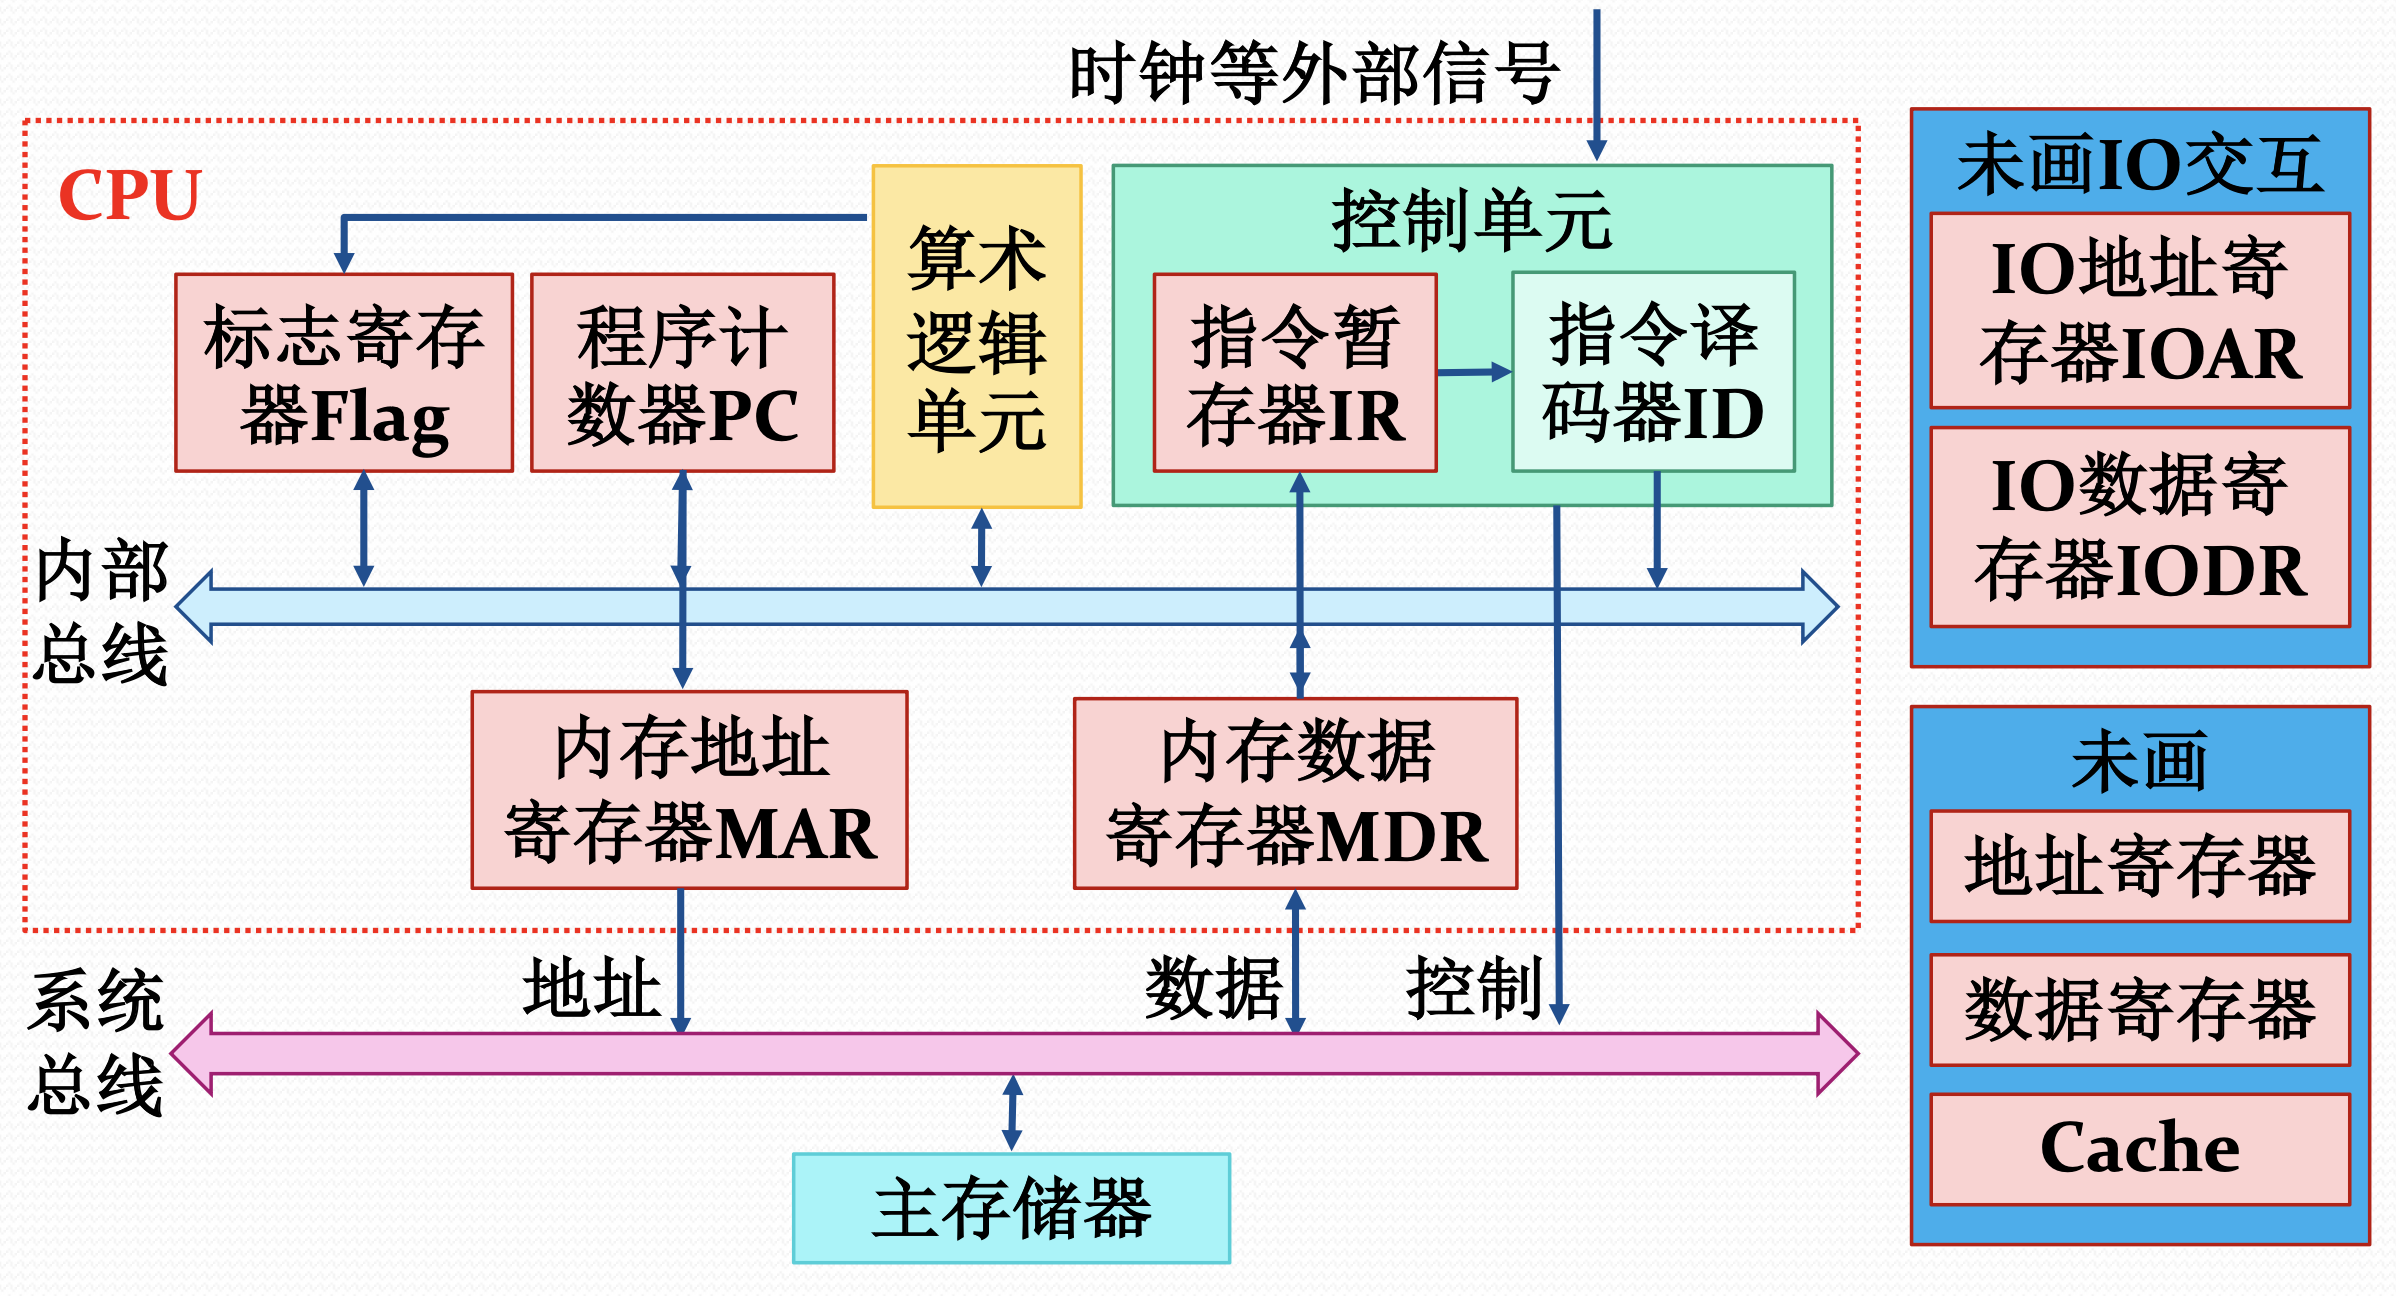
\includegraphics[width=0.75\textwidth]{img/2.1.1.1}
	\end{figure}
	\begin{itemize}
		\item 上图各组件通过内部总线连接起来,构成一个不包含通用寄存器、I/O 相关寄存器、地址寄存器、数据寄存器和 Cache 的示意图
		\item CPU 中的各组件描述
		\begin{itemize}
			\item 算数逻辑单元:计算结束之后会将结果的标志放置到标志寄存器 Flag 中
			\item 控制单元:包含重要的指令译码器 ID,而指令是放置在指令暂存器 IR 中
			\item 程序计数器 PC:下一条指令的地址
			\item 内存地址寄存器和内存数据寄存器:用来完成对内存数据的访问
		\end{itemize}
		\item 通过系统总线来访问内存中的数据,首先设置地址和数据,然后通过控制来完成数据的读取和写回
		\item 时钟等来源于外围设备等信号直接反应到控制单元中,中断响应操作由此可以实现
	\end{itemize}


	\subsubsection{寄存器}
	寄存器分为\textbf{用户程序可见寄存器}和\textbf{状态与控制寄存器}两类
	\begin{itemize}
		\item 用户程序可见寄存器
		\begin{itemize}
			\item 可以使程序员减少访问主存储器的次数,提高指令执行的效率
			\item 所有程序可使用,包括应用程序和系统程序
			\begin{itemize}
				\item 数据寄存器:又称通用寄存器
				\item 地址寄存器:索引、栈指针、段地址等寄存器
			\end{itemize}
		\end{itemize}
		\item 状态与控制寄存器
		\begin{itemize}
			\item 用于控制处理器的操作;主要被具有特权的操作系统程序使用,以控制程序的执行
			\begin{itemize}
				\item 程序计数器 PC:存储将取指令的地址
				\item 指令寄存器 IR:存储最近使用的指令
				\item 条件码 CC:CPU 为指令操作结果设置的位,标志正/负/零/溢出等结果
				\item 标志位
				\begin{table}[H]
					\centering
					\begin{tabular}{|l|l|}
					\hline
					\multicolumn{1}{|c|}{位} & \multicolumn{1}{c|}{描述} \\ \hline
					中断位                     & 是否有中断发生了,中断源是什么         \\ \hline
					中断允许位                   & 表示目前是否响应中断              \\ \hline
					中断屏蔽位                   & 中断发生了,中断响应了,我们要不要屏蔽中断   \\ \hline
					处理器模式位                  & 现在处理器是处于何种模式            \\ \hline
					内存保护位                   & 对这段内存是只读还是读写还是不可操作      \\ \hline
					\end{tabular}
					\end{table}
			\end{itemize}
		\end{itemize}
	\end{itemize}

	\subsubsection{程序状态字}
	\begin{itemize}
		\item PSW 既是操作系统的概念,指记录当前程序运行的\textbf{动态信息},通常包含:
		\begin{itemize}
			\item 程序计数器、指令寄存器、条件码
			\item 中断字、中断允许/禁止、中断屏蔽、处理器模式、内存保护、调试控制
		\end{itemize}
		\item PSW 也是计算机系统的\textbf{寄存器}
		\begin{itemize}
			\item 通常设置一组控制与状态寄存器
			\item 也可以专设一个 PSW 寄存器
		\end{itemize}
	\end{itemize}


	\subsection{指令与处理器模式}
	\subsubsection{机器指令及流水线}
	\textbf{机器指令}是计算机系统执行的基本命令,是中央处理器执行的基本单位
	\begin{itemize}
		\item 指令由一个或多个字节组成,包括操作码字段、一个或多个操作数地址字段、以及一些表征机器状态的状态字以及特征码
		\item 指令完成各种算术逻辑运算、数据传输、控制流跳转
	\end{itemize}

	指令执行过程
	\begin{itemize}
		\item CPU 根据 PC \textbf{取出指令},放入 IR,并对指令译码,然后发出各种控制命令,执行微操作系列,从而完成一条指令的执行
		\item 指令执行步骤如下:(仅为一种划分方式)
		\begin{itemize}
			\item 取指:根据 PC 从存储器或高速缓冲存储器中取指令到 IR
			\item 解码:解译 IR 中的指令来决定其执行行为
			\item 执行:连接到 CPU 部件,执行运算,产生结果并写回,同时在 CC 里设置运算结论标志;跳转指令操作PC,其他指令递增 PC 值
		\end{itemize}
	\end{itemize}
	\begin{figure}[H]
		\centering
		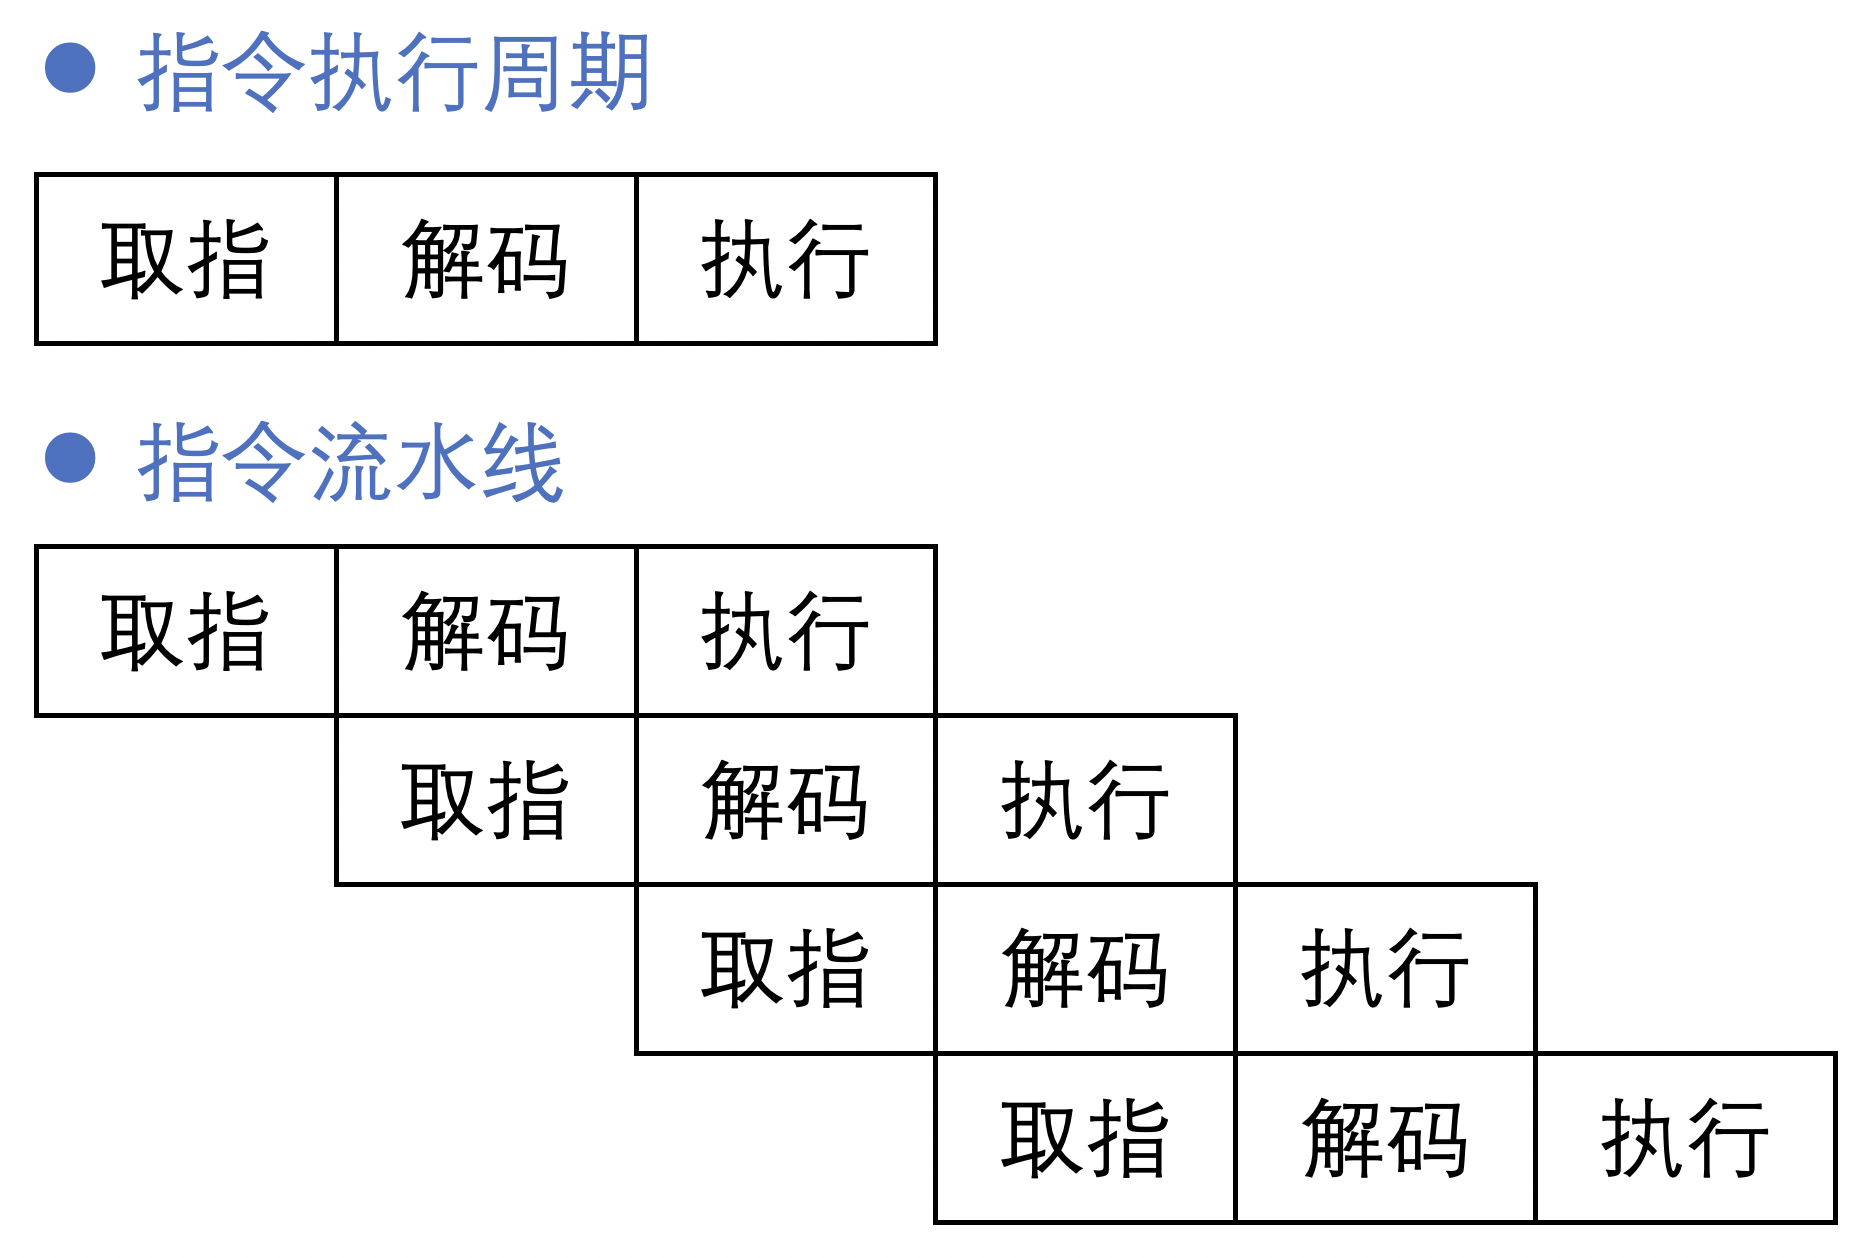
\includegraphics[width=0.5\textwidth]{img/2.1.2.1}
	\end{figure}

	\subsubsection{特权指令和非特权指令}
	用户程序并非能够使用全部机器指令,那些与计算机核心资源相关的特殊指令会被保护
	\begin{itemize}
		\item 比如:启动 I/O 指令、置 PC 指令等
		\item 核心资源相关的指令只能被操作系统程序使用
	\end{itemize}

	在多道程序设计环境中,从资源管理和控制程序执行的角度出发,必须将指令系统中的指令分成两类:
	\begin{itemize}
		\item 特权指令:只能被操作系统内核使用的指令
		\item 非特权指令:能够被所有程序使用的指令
	\end{itemize}


	\subsubsection{内核态和用户态}
	\textbf{内核态}又称\textbf{管态},是操作系统管理程序运行时所处的状态
	\begin{itemize}
		\item 可认为处理器正在运行可信系统软件,此时全部机器指令都被允许在处理器上执行
		\item 程序可访问所有主存单元和系统资源,并具有改变处理器状态的能力
	\end{itemize}

	\textbf{用户态}又称\textbf{目态},当处理器处于用户态时,它正在运行非可信的应用程序,此时无法执行特权指令,且访问仅限于当前处理器上执行程序所在的地址空间
	
	处理器、主存、设备等资源管理程序应在内核态运行,否则安全性没有保证
	\begin{itemize}
		\item 涉及核心数据结构的各种原语应在内核态运行,否则会导致系统混乱
		\item 创建进程管理数据结构、为进程分配主存、启动外围设备构造文件系统核心数据等程序也必须在内核态运行
	\end{itemize}

	应用程序逻辑与数据处理则应放在用户态执行
	\begin{itemize}
		\item 操作系统外外围程序,如支撑程序、命令解释程序、页面调度程序、图形界面处理程序、记账程序与审计程序等也可以在用户态运行
	\end{itemize}

	计算机系统为操作系统提供内核态与用户态的界分,通过设置处理器状态实现特权指令管理
	\begin{itemize}
		\item 通过为处理器建立硬件标志位,称为处理器状态位,通常是程序状态字中的比特位
		\item 处理器状态位可以定义操作系统的保护权限
		\begin{itemize}
			\item 当其为内核态时,处理器就可以执行包括特权指令在内的所有指令,这一状态为操作系统内核程序使用
			\item 当处理器状态位设置为用户态时,处理器就只能执行非特权指令,应用程序和操作系统外围程序在此状态下被良好隔离、互不打扰
		\end{itemize}
	\end{itemize}

	大多数计算机系统的处理器状态有4种,分别支持 0$\sim$3 级共 4 个特权级别,其中 0 级权限最高,3 级权限最低:
	\footnote{目前几乎所有通用操作系统实现都只使用了 0 级与 3 级,即简单区分内核态与用户态}
	\begin{itemize}
		\item 0 级为内核级,处理 I/O 操作,执行中断处理等关键操作
		\item 1 级为系统调用级,可以执行文件系统调用,获得特定的和受保护的程序服务
		\item 2 级为共享库级,可被多个运行进程共享,允许调用库函数,读取但不修改内部数据
		\item 3 级为应用程序级,所受到的保护最少
	\end{itemize}

	\subsubsection{处理器状态切换}
	只有\textbf{中断}才会使处理器从用户态向内核态转换,其中包含以下三类情况:
	\begin{itemize}
		\item 在程序运行时产生异步中断事件(如 I/O 操作完成),运行程序被中断,转向中断处理程序处理
		\item 程序主动同步请求操作系统服务,执行系统调用,触发了系统异常,也称白愿性中断
		\item 在程序运行时,执行指令出现问题从而产生同步异常事件(如用户态执行特权指令),运行程序被打断,转向异常处理程序工作,这属于程序性中断事件
	\end{itemize}
	操作系统内核处理完成后,调用中断返回指令(例如 Intel 的 \verb|iret| 指令),实现从内核态返回用户态,操作系统将控制权转交给应用进程
	\begin{figure}[H]
		\centering
		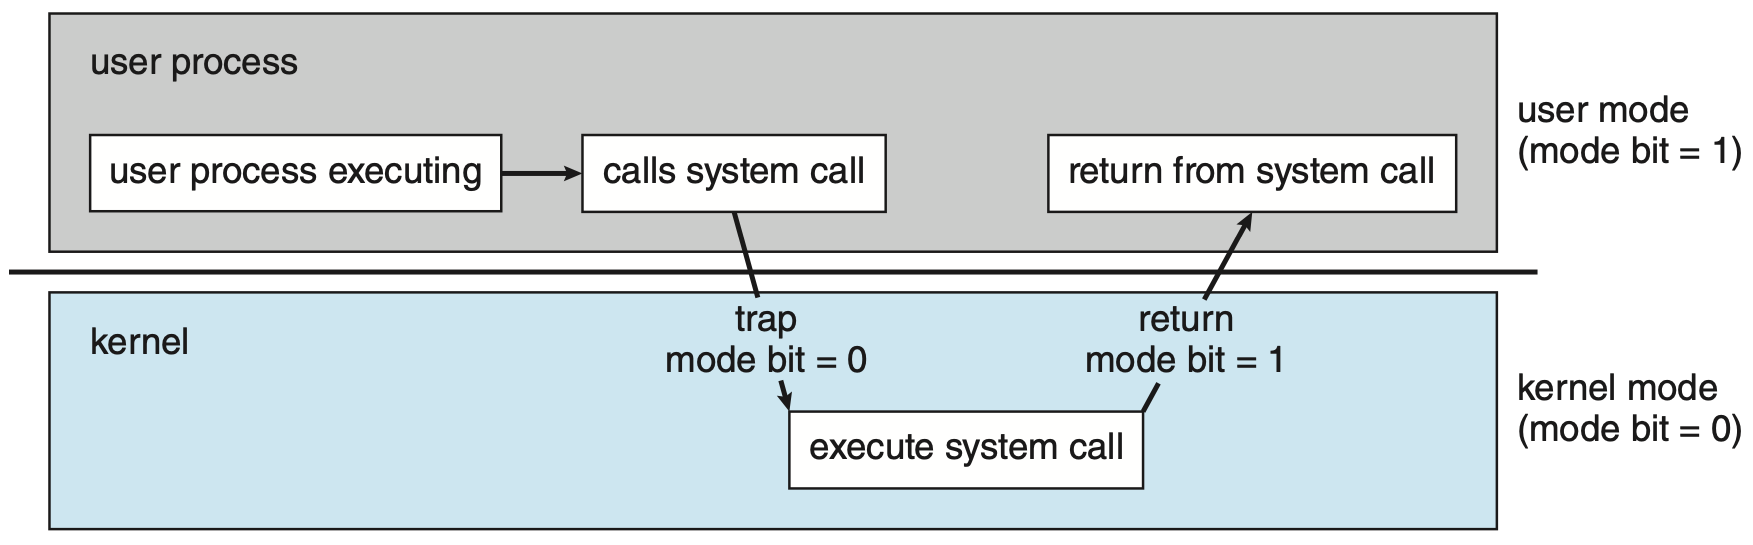
\includegraphics[width=0.7\textwidth]{img/2.1.2.4}
	\end{figure}

	\subsubsection{用户栈和核心栈}
	用户栈是用户进程空间中开辟的一块区域,用于保存应用程序的子程序(函数)间相互调用的参数、返回值、返回点以及子程序的局部变量
	如果只有用户栈,没有核心栈,那么操作系统的一切工作都将暴露在用户态下,将很难提供相应的保护措施
	核心栈也叫系统栈或内核栈,是内存中属于操作系统空间的一块区域,其用途包括:
	\begin{itemize}
		\item 保存中断现场,对于嵌套中断,将被中断程序的现场信息依次压入核心栈,中断返回时逆序弹出
		\item 保存操作系统程序(函数)间相互调用的参数、返回值、返回点以及程序局部变量
	\end{itemize}
	每个进程被创建时捆绑一个核心栈,具有可读、可写、不可执行的属性

	\section{中断}
	\subsection{中断的概念}
	中断是指程序执行过程中,遇到急需处理的事件时,暂时中止 CPU 上现行程序的运行,转去执行相应的事件处理程序,待处理完成后再返回原程序被中断处或调度其他程序执行的过程
	\begin{itemize}
		\item 中断有广义和狭义之分,上述中断是指广义的中断
		\item 广义中断可以划分为狭义中断、异常和系统异常三大类
		\begin{itemize}
			\item 狭义的中断(很多情况下简称为中断)指来源于处理器之外的中断事件,即与当前运行指令无关的中断事件,如 I/O 中断、时钟中断、外部信号中断等
			\item 异常指当前运行指令引起的中断事件,如地址异常、算术异常、处理器硬件故障等
			\item 系统异常指执行陷入指令而触发系统调用引起的中断事件,如请求设备、请求 I/O、创建进程等
		\end{itemize}
	\end{itemize}
	操作系统是“中断驱动”的;换言之,中断是激活操作系统的唯一方式


	\subsection{中断源}
	通常将引起中断的事件,即中断请求信号的来源,统称为中断源

	中断事件可以分为以下几类:硬件故障中断事件、程序性中断事件、自愿性中断事件、I/O 中断事件和外部中断事件

	\subsubsection{硬件故障中断事件}
	\begin{itemize}
		\item 由处理器、内存储器、总线等硬件故障引起,除了极少类的校验错误可以恢复以外,是\textbf{非常严重}的中断
		\item 处理原则为:保护现场,停止设备,停止 CPU,向操作员报告,等待人工干预
	\end{itemize}


	\subsubsection{程序性中断事件}
	由处理器执行机器指令出错或异常引起
	\begin{itemize}
		\item 除数为零、操作数溢出等算术异常:简单处理,报告用户,由用户判断计算机结果是否可信;也可以由用户编写中断续元程序处理,操作系统把处理权限交给用户程序
		\item 非法指令、用户态使用特权指令、地址越界、非法存取等指令异常:终止进程
		\item 终止进程指令:终止进程
		\item 虚拟地址异常:指令和数据不在内存当中,调整内存后重新执行指令
	\end{itemize}

	\subsubsection{自愿性中断事件}
	此类中断事件又称系统调用,是由程序执行陷入指令引起的,表示当前运行程序对操作系统功能的调用
	\begin{enumerate}[label=\arabic*.]
		\item 程序执行陷入指令,并通过适当方式指明系统调用号
		\item 通过系统陷阱机制进入系统调用处理程序,现场信息被保护到核心栈,按功能号实现跳转
		\item 通过系统调用入口表找到相应系统调用服务历程的入口地址
		\item 执行系统调用服务例程,结束后返回系统调用的下一条指令
	\end{enumerate}


	\subsubsection{I/O中断事件}
	来源于外围设备报告 I/O 状态的中断事件
	\begin{itemize}
		\item I/O 操作正常结束:本进程设置为就绪态,让等待传输的下一个进程占有设备或通道并启动数据传输
		\item I/O 操作发生故障:先向设备发送命令索取状态字,分析产生故障的确切原因,再执行复执或请求人工干预
		\item I/O 操作发生异常:分析情况,采取相应措施并向操作员报告,如通知操作员换卷、装纸等
	\end{itemize}

	\subsubsection{外部中断事件}
	此类中断事件来自 CPU 现场之外的信号
	\begin{itemize}
		\item 时钟中断:计时
		\item 间隔时钟中断:时间片到,被中断的进程就要让出处理器进入就绪队列
		\item 设备报到与结束中断:调整设备表
		\item 键盘/鼠标信号中断:根据信号作出相应反应
		\item 关机/重启动中断:写回文件,停止设备与 CPU
	\end{itemize}


	\subsection{中断系统}
	\begin{itemize}
		\item 中断系统是计算机系统中响应和处理中断的系统,包括硬件子系统和软件子系统两部分
		\begin{itemize}
			\item 中断响应由硬件子系统完成
			\item 中断处理由软件子系统完成
		\end{itemize}
		\item 中断系统是操作系统的基础,中断系统也是软硬件协同系统的典型例子
	\end{itemize}


	\subsubsection{中断响应}
	在指令执行周期最后增加一个微操作,以响应中断
	\begin{figure}[H]
		\centering
		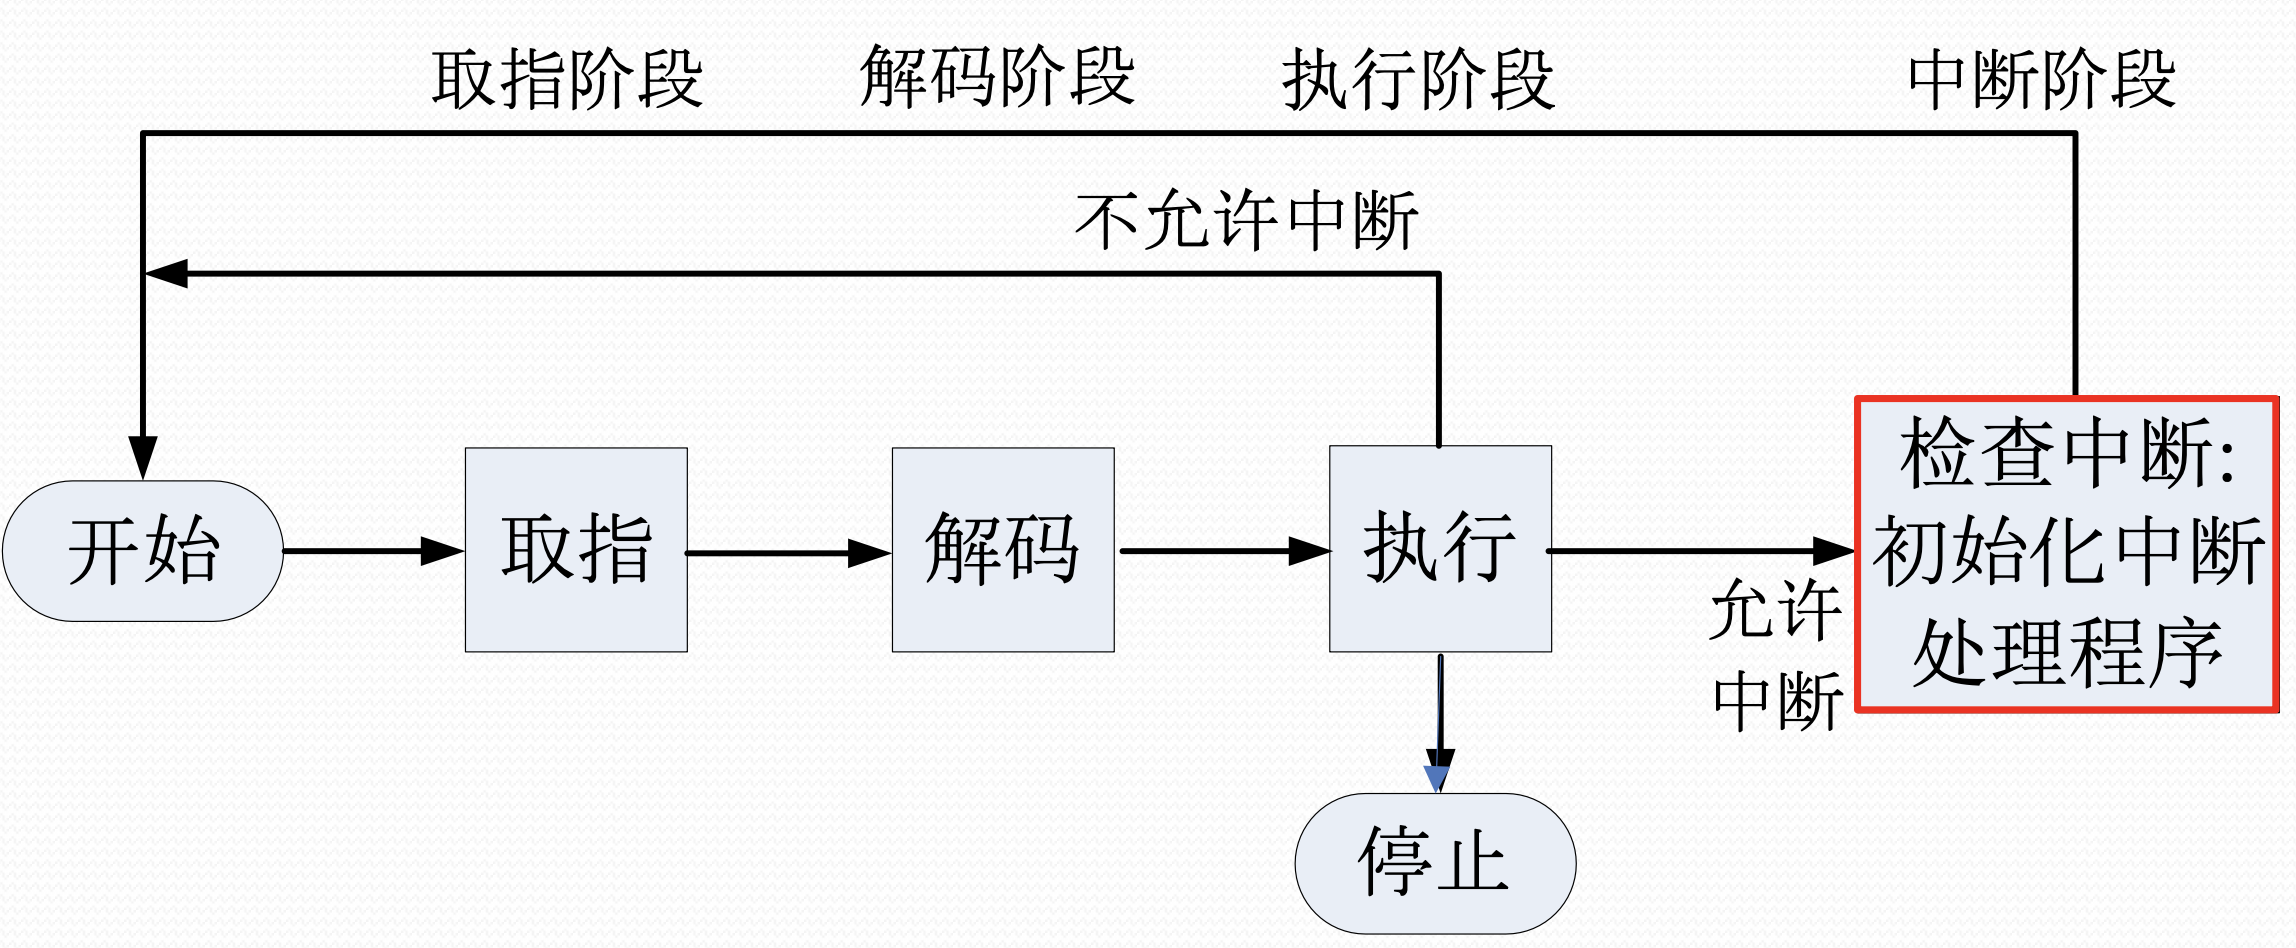
\includegraphics[width=0.7\textwidth]{img/2.2.3.1}
	\end{figure}
	计算机系统中发现并响应中断、异常的硬件装置称为中断装置。由于中断源的多样性,硬件实现的中断装置有多种,分别处理不同类型的中断:
	\begin{itemize}
		\item 处理器外的中断:由中断控制器发现和响应
		\begin{itemize}
			\item 中断控制器是 CPU 中的一个控制部件,包括中断控制逻辑电路和中断寄存器
			\begin{itemize}
				\item 外部设备向其发出中断请求 IRQ,在中断寄存器中设置已发生的中断
				\item 指令处理结束前,会检查中断寄存器,若有不被屏蔽的中断产生,则改变处理器内操作的顺序,引出操作系统中的中断处理程序
			\end{itemize}
		\end{itemize}
		\item 处理器内的异常:由指令的控制逻辑和实现线路发现和响应,相应机制称为陷阱
		\begin{itemize}
			\item 执行指令出现异常后,会根据异常情况转向操作系统的异常处理程序
			\item 出现虚拟地址异常后,需要重新执行指令, 往往越过陷阱独立设置页面异常处理程序
		\end{itemize}
		\item 请求操作系统服务的系统异常:处理器执行陷入指令时直接触发,相应机制称为系统陷阱
		\begin{itemize}
			\item 执行陷入指令后,越过陷阱处理,触发系统陷阱,激活系统调用处理程序
		\end{itemize}
	\end{itemize}

	中断/异常响应过程
	\begin{itemize}
		\item 发现中断源,提出中断请求(选择响应哪一个程序)
		\begin{itemize}
			\item 发现中断寄存器中记录的中断
			\item 决定这些中断是否被屏蔽
			\item 当有多个要响应的中断源时,根据规定的优先级选择一个
		\end{itemize}
		\item 中断当前程序的执行(保护现场)
		\begin{itemize}
			\item 保存当前程序的 PSW/PC 到核心栈
		\end{itemize}
		\item 转向操作系统的中断处理程序
		\begin{itemize}
			\item 处理器状态已从用户态转换至内核态
		\end{itemize}
		\item 恢复现场
		\begin{itemize}
			\item 恢复原运行程序的 PSW,重新返回中断点,以便执行后续指令
		\end{itemize}
	\end{itemize}


	\subsubsection{中断处理程序}
	中断处理程序是操作系统处理中断事件的控制程序,主要任务是处理中断事件和恢复正常操作

	处理中断包括以下 4 项主要内容:
	\begin{enumerate}[label=\arabic*.]
		\item 保护未被硬件保护的处理器状态
		\item 通过分析被中断进程的 PSW 中断码字段, 识别中断源
		\item 分别处理发生的中断事件
		\item 恢复正常操作
	\end{enumerate}

	恢复正常操作包括两种情况:
	\begin{itemize}
		\item 对于某些能够被快速处理的中断,在处理完毕后,直接返回刚刚被中断的进程
		\item 对于其他一些中断,需要中断当前进程的运行,调整进程队列,启动进程调度,选择下一个执行的进程并恢复其执行
	\end{itemize}


	\subsubsection{中断系统的总体处理流程}
	\begin{figure}[H]
		\centering
		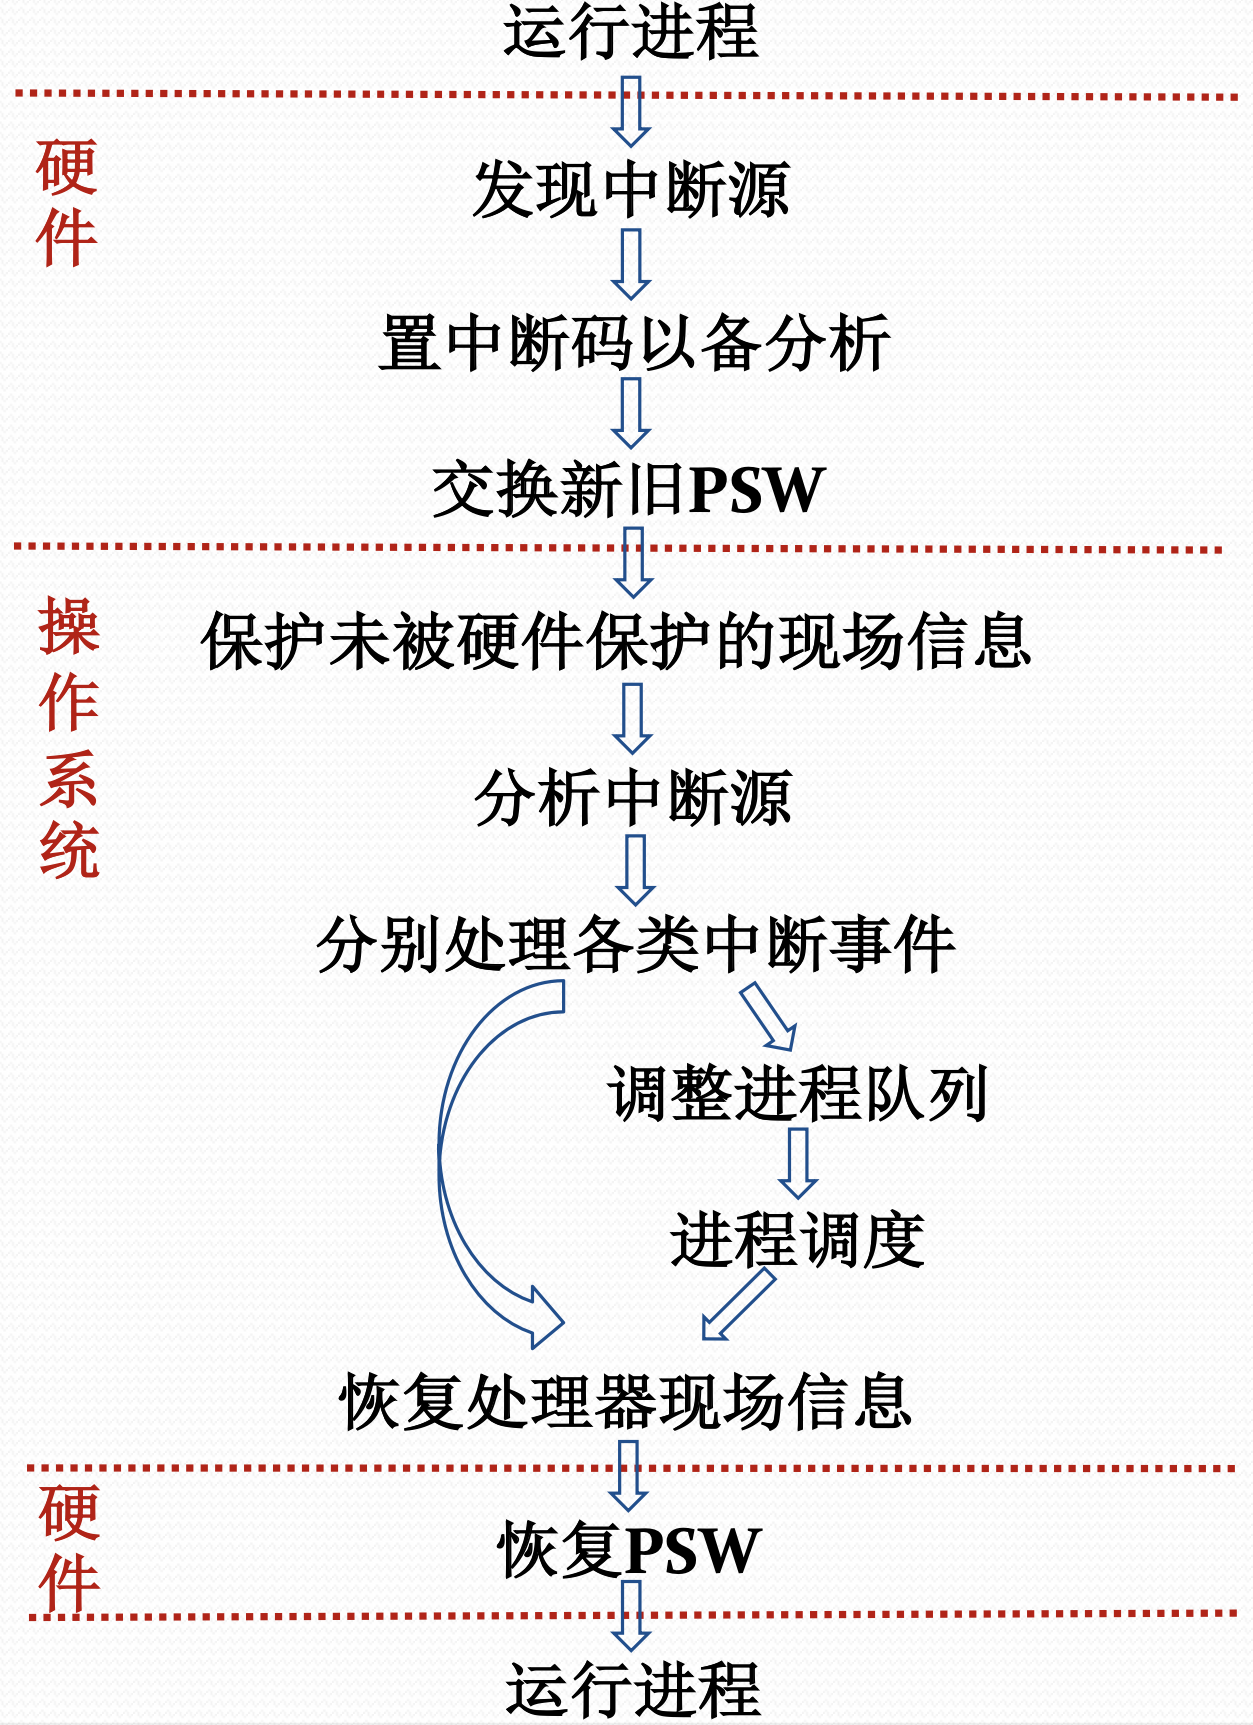
\includegraphics[width=0.6\textwidth]{img/2.2.3.3}
	\end{figure}


	\subsection{多中断的响应与处理}
	\subsubsection{中断屏蔽}
	中断屏蔽是指禁止 CPU 响应中断或者禁止产生中断
	\begin{itemize}
		\item 前者指硬件产生中断请求后,CPU 暂时不予响应,一直等到中断开放后,被屏蔽的中断才能被响应并获得处理
		\begin{itemize}
			\item 常用在处理某个中断时,如处理一个 I/O 中断的关键时刻,防止其他中断干扰
		\end{itemize}
		\item 后者指当引起中断的事件发生时,硬件不允许提出中断请求,故由于中断被禁止而不可能产生中断
		\begin{itemize}
			\item 通常设备中断、时钟中断等可以被暂时禁止
		\end{itemize}
	\end{itemize}

	中断屏蔽有如下作用:
	\begin{itemize}
		\item 延迟或禁止某些中断的响应,系统程序执行过程中不希望产生干扰事件,以免共享数据结构受到破坏
		\item 协调中断响应与中断处理的关系,确保高优先级中断可以打断低优先级中断,反之却不能
		\item 防止同级中断相互干扰,在处理某优先级中断事件时必须屏蔽该级中断,以免造成混乱
	\end{itemize}


	\subsubsection{中断优先级}
	中断优先级指的是当计算机同时检测到多个中断时,中断装置响应中断的顺序
	\begin{itemize}
		\item 有优先度的响应中断:将紧迫程度相当的中断源归为同一级别,将紧迫程度差距较大的中断源归为不同级别
		\item 一种可能的处理次序:
		\begin{itemize}
			\item 处理机硬件故障中断事件
			\item 自愿性中断事件
			\item 程序性中断事件
			\item 时钟中断等外部中断事件
			\item 输入输出中断事件
			\item 重启动和关机中断事件
		\end{itemize}
		\item 不同类型的操作系统有不同的中断优先级
		\begin{itemize}
			\item PC 做出关机操作表示放弃当前的所有的操作,所以重启动和关机中断是优先级最高的中断
		\end{itemize}
	\end{itemize}

	\subsection{多重中断事件处理}
	\begin{itemize}
		\item 当计算机响应中断后,在中断处理过程中,可以再响应其他中断
		\item 操作系统是性能攸关的程序系统,且中断响应处理有硬件要求,考虑系统效率和实现代价问题,中断的嵌套处理应限制在一定层数内,一般以不超过三层为宜
		\item 中断的嵌套处理改变中断处理次序,先响应的有可能后处理
		\item 决定中断处理次序的因素
		\begin{itemize}
			\item 中断屏蔽可以使中断装置不响应某些中断
			\item 中断优先级决定了中断装置响应中断的次序
			\item 中断可以嵌套处理,但嵌套的层数应有限制
			\item 中断的嵌套处理改变了中断处理的次序
		\end{itemize}
	\end{itemize}
	\begin{figure}[H]
		\centering
		\includegraphics[width=0.7\textwidth]{img/2.2.4.3}
	\end{figure}


	\section{进程管理}
	\subsection{进程及其状态}

	\subsubsection{进程的概念}
	操作系统必须全方位地管理计算机系统中运行的程序。因此,操作系统为正在运行程序建立一个管理实体:\textbf{进程}
	\begin{itemize}
		\item \textbf{进程是一个具有一定独立功能的程序关于某个数据集合的一次运行活动}
		\begin{itemize}
			\item 具有一定独立功能的程序:进程是相对独立的
			\item 关于某个数据集合:对于不同数据集合的操作不是同一个进程
			\item 一次运行活动:有生命周期
		\end{itemize}
		\item \textbf{进程是操作系统进行资源分配和调度的一个独立单位}:这只限于单线程单进程的情况下
		\begin{itemize}
			\item 资源分配:除了 CPU 之外的资源的分配,比如内存和外设等
			\item 单线程情况下,进程的资源分配和调度就是处理器的
			\item 调度特指处理器的调度
		\end{itemize}
		\item 进程可以看为可运行程序加载到内存,配合相应的数据集,在操作系统中的一个实例,程序可以多次被加载进入成为进程
		\item 进程的属性:
		\begin{itemize}
			\item \textbf{动态性}:进程是程序在数据结合上的一次执行过程,是动态概念,同时它有生命周期,而程序是一组有序指令序列,是静态概念,所以程序作为系统中的一种资源是永久存在的
			\item \textbf{共享性}:同一程序同时运行于不同数据集合上时都是不同的进程,即不同的进程可以运行相同的程序
			\item \textbf{独立性}:每个进程是操作系统中的一个独立实体。有自己的虚存空间、程序计数器和内部状态
			\item \textbf{制约性}:进程因共享资源或协同工作产生相互制约关系,造成进程执行速度的不可预测性,必须对进程的执行次序或相对执行速度予以协调
			\item \textbf{并发性}:多个进程的执行在时间上可以重叠
		\end{itemize}
		\item 一个进程包括五个实体部分,分别是:
		\begin{itemize}
			\item (操作系统管理运行程序的)数据结构 P
			\item (运行程序的)内存代码 C
			\item (运行程序的)内存数据 D
			\item (运行程序的)通用寄存器信息 R
			\item (操作系统控制程序执行的)程序状态字信息 PSW
		\end{itemize}
	\end{itemize}
	\begin{figure}[H]
		\centering
		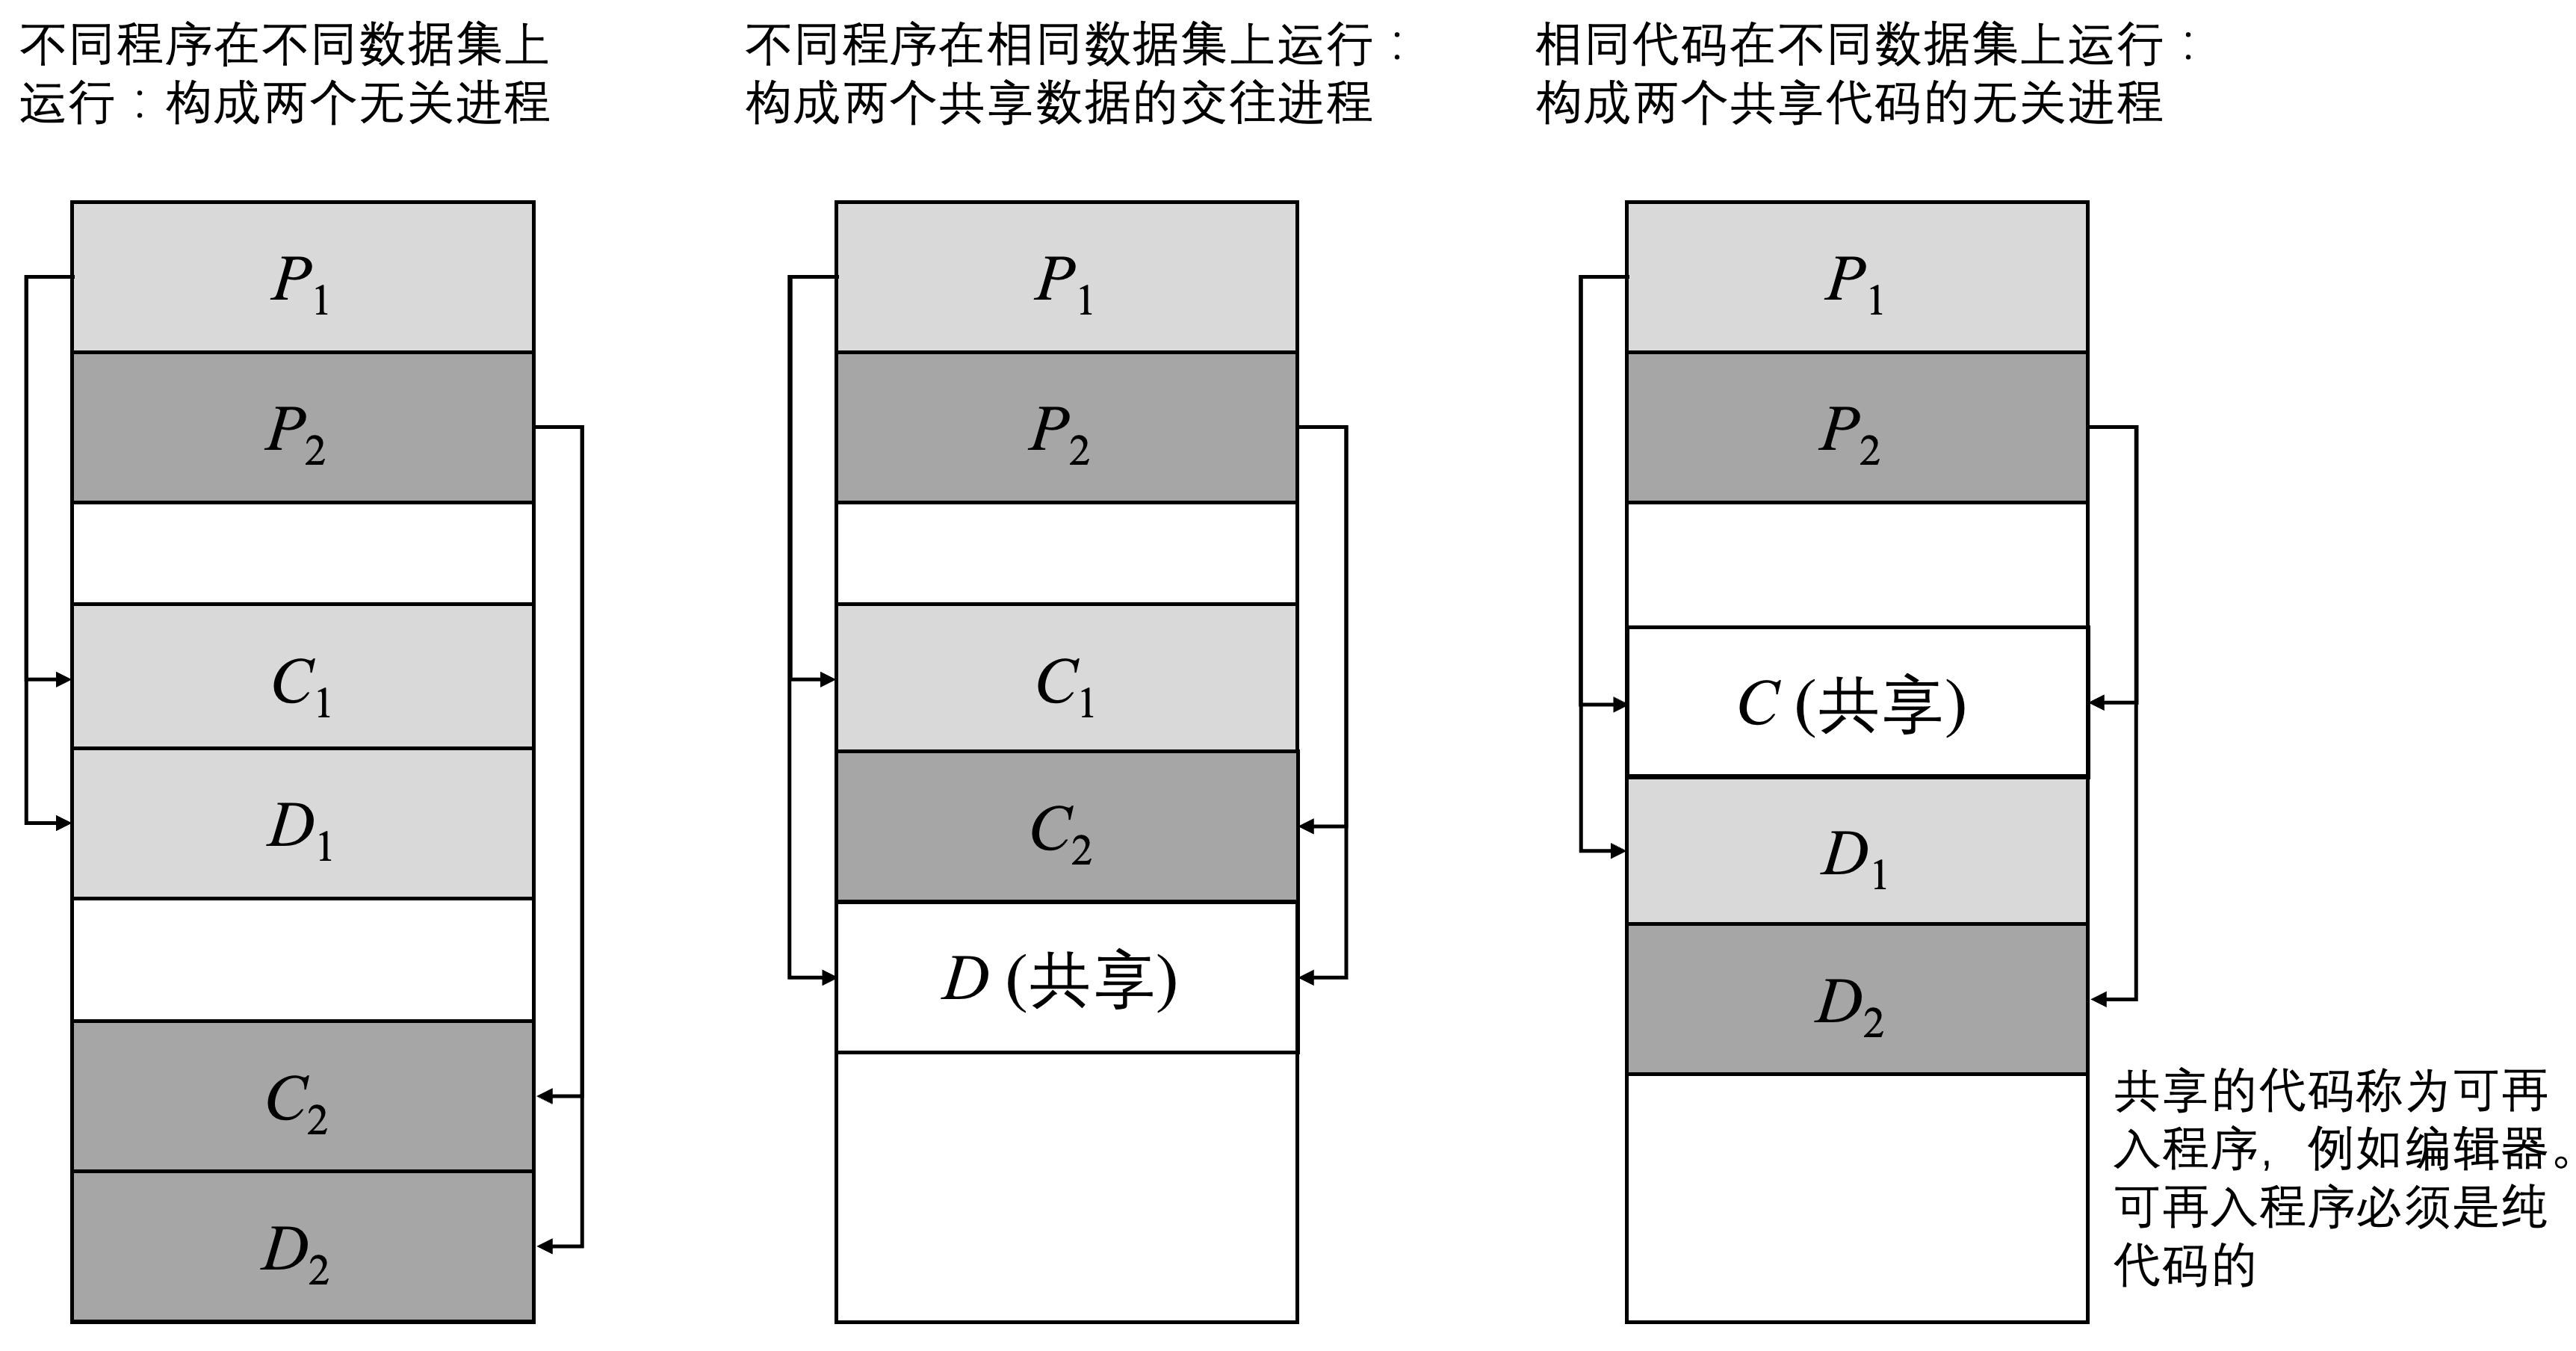
\includegraphics[width=0.65\textwidth]{img/2.3.1.1}
	\end{figure}


	\subsubsection{进程的状态}
	在概念层次,进程在执行过程中要定义\textbf{运行}、\textbf{就绪}和\textbf{等待}三种进程状态\footnote{处于运行态的进程个数不能大于处理器个数,处于就绪态和等待态的进程可以有多个}
	\begin{itemize}
		\item 运行(running)态:进程占有处理器正在运行的状态
		\item 就绪(ready)态:进程具备运行条件,等待系统分配处理器以便运行的状态
		\item 等待(waiting)态:又称阻塞(blocked)态或睡眠(sleep)态,指进程不具备运行条件等待某个事件完成的状态
	\end{itemize}
	\begin{figure}[H]
		\centering
		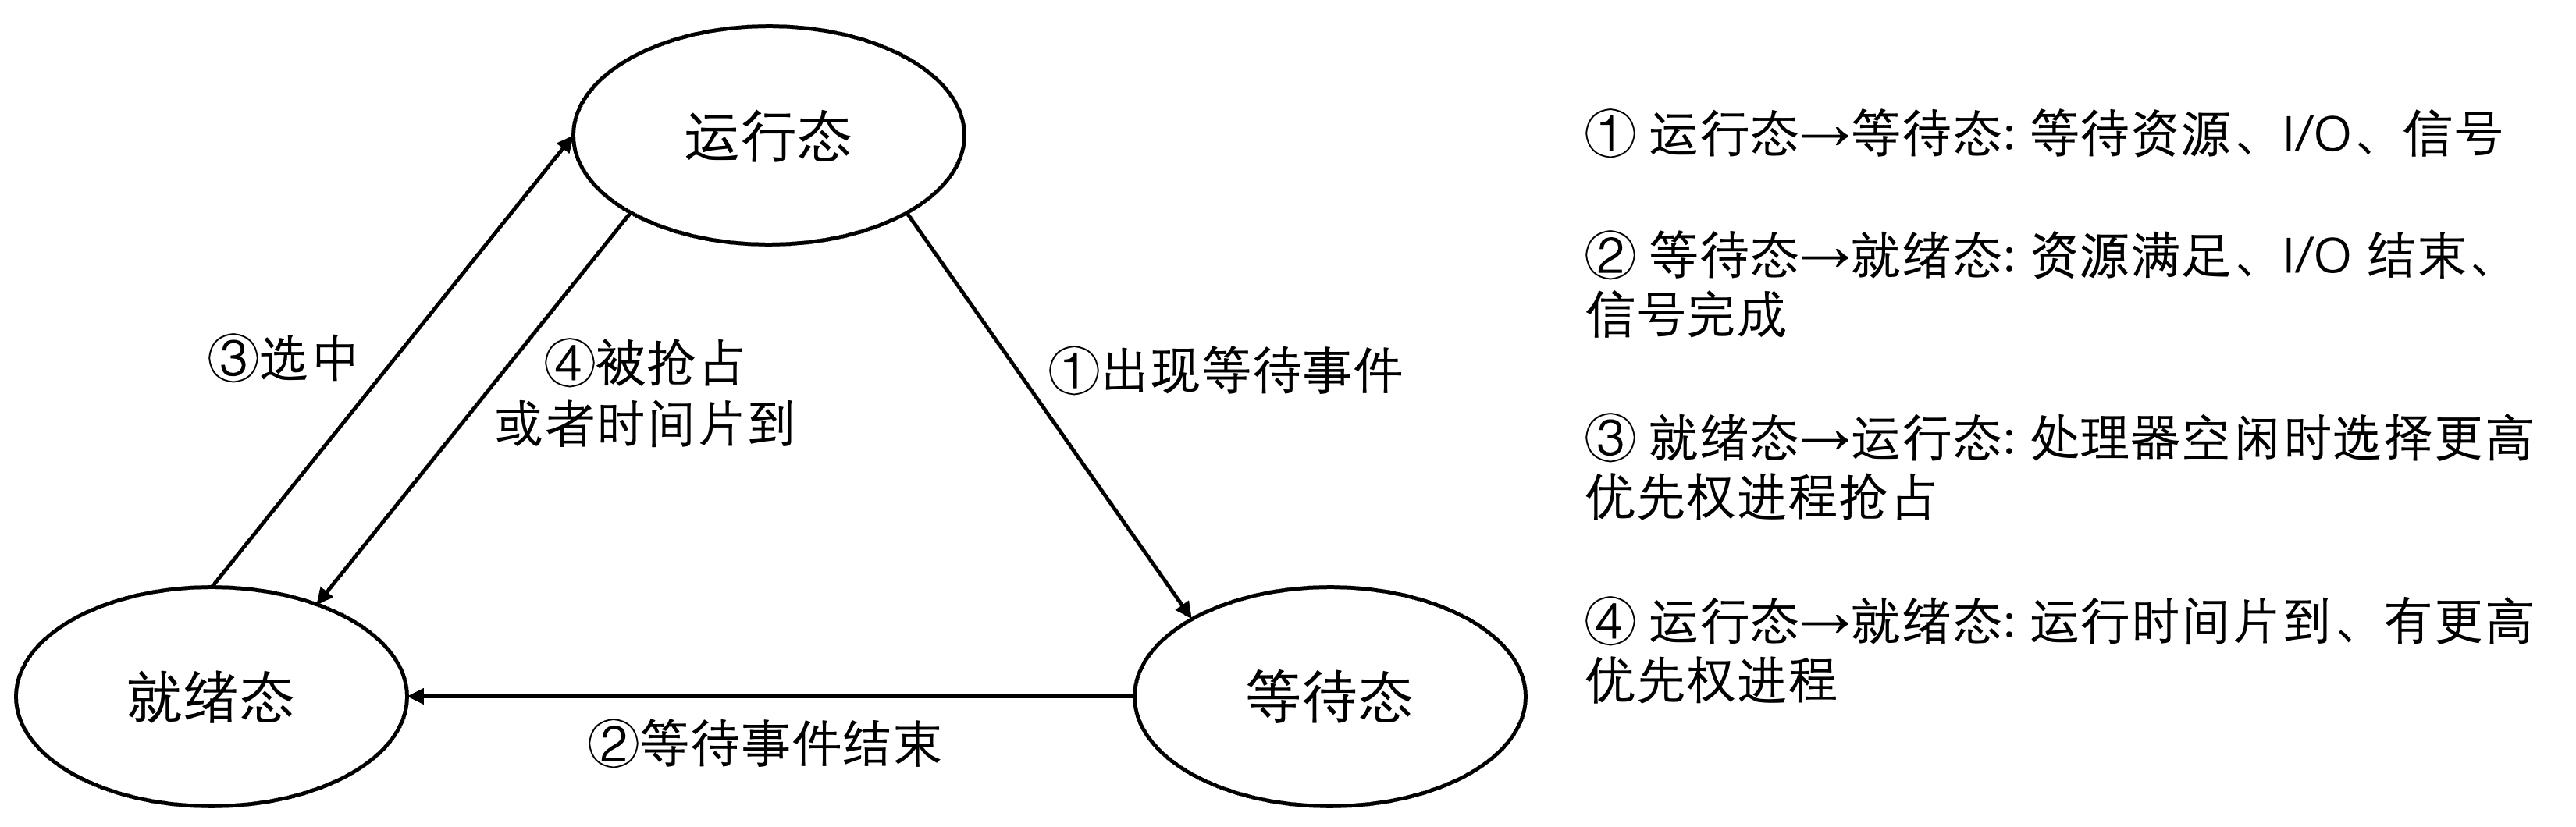
\includegraphics[width=0.95\textwidth]{img/2.3.1.2.1}
	\end{figure}
	
	在操作系统实现层面,进程的创建和撤销都不是一蹴而就的,因而需要增加\textbf{新建}(new)态和\textbf{终止}(exit)态
	\begin{itemize}
		\item 新建态对应于进程被创建时所处的状态,此时进程尚未进入就绪队列
		\begin{itemize}
			\item 创建进程包含两个步骤:为新进程分配所需资源及建立必要的管理信息,设置该进程为就绪态并等待被调度执行
		\end{itemize}
		\item 终止态是指进程完成任务到达正常结束点,或出现无法克服的错误而异常终止,或被操作系统及有终止权的进程所终止时所处的状态
		\begin{itemize}
			\item 处于终止态的进程不再被调度执行,下一步将被系统撤销,最终从系统中消失
			\item 终止进程也包含两个步骤:等待操作系统或相关进程进行后续处理,回收占用的资源并被系统删除
		\end{itemize}
	\end{itemize}

	上述概念都是假设所有进程在主存中。事实上可能会出现这样一些情况:
	\begin{itemize}
		\item 由于不断创建进程,系统资源特别如主存资源等已不能满足进程运行的要求,此时必须将某些进程\textbf{挂起}(suspend)并对换到磁盘对换区中,释放它占有的某些资源,暂时不参与低级调度,以此达到平滑系统负荷的目的
		\item 系统出现故障,需要暂时挂起一些进程,以便故障消除后再解除挂起并恢复进程运行
		\item 用户调试程序的过程中可以请求挂起该进程,以便进行某些检查和修改
	\end{itemize}

	所以就引入了两个新状态:\textbf{挂起就绪态}(ready suspend)和\textbf{挂起等待态}(blocked suspend)
	\begin{itemize}
		\item 挂起就绪态表明进程具备运行条件,但目前在外存中,只有当它被对换到主存才能被调度执行
		\item 挂起等待态则表明进程正在等待某一个事件发生且在外存中
	\end{itemize}

	挂起进程等同于不在主存的进程,因此,挂起进程将不参与处理器调度,直到它们被对换进主存

	\begin{figure}[H]
		\centering
		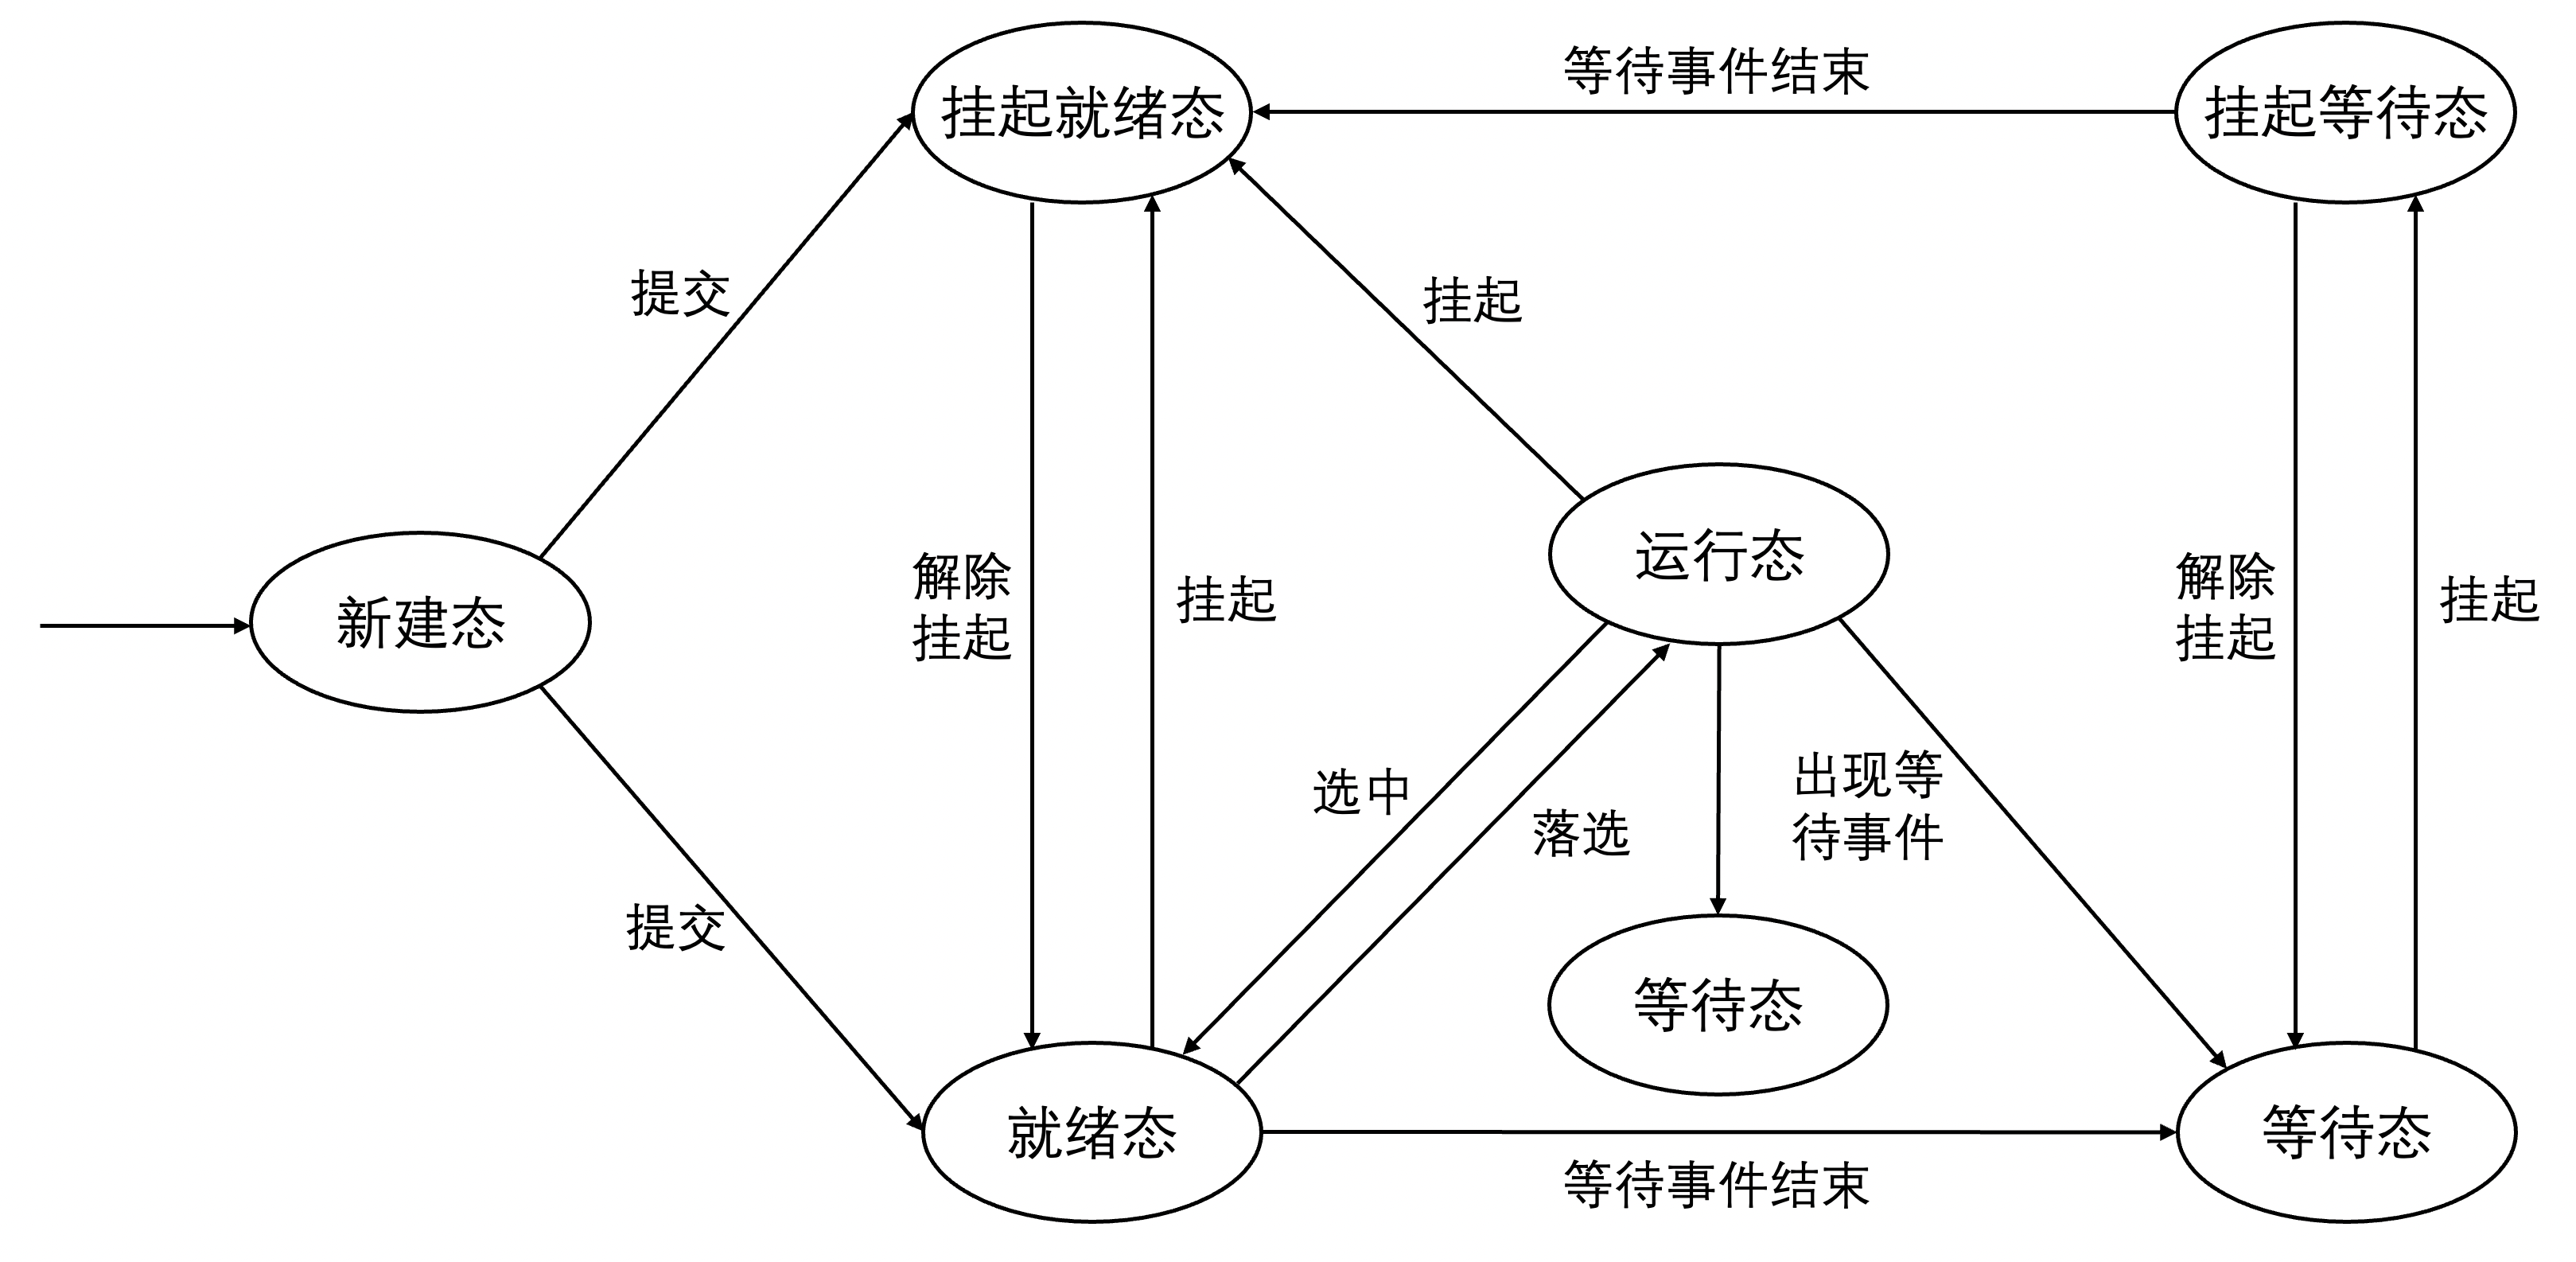
\includegraphics[width=0.6\textwidth]{img/2.3.1.2.2}
	\end{figure}

	\subsubsection{SVR4进程状态模型}
	\begin{figure}[H]
		\centering
		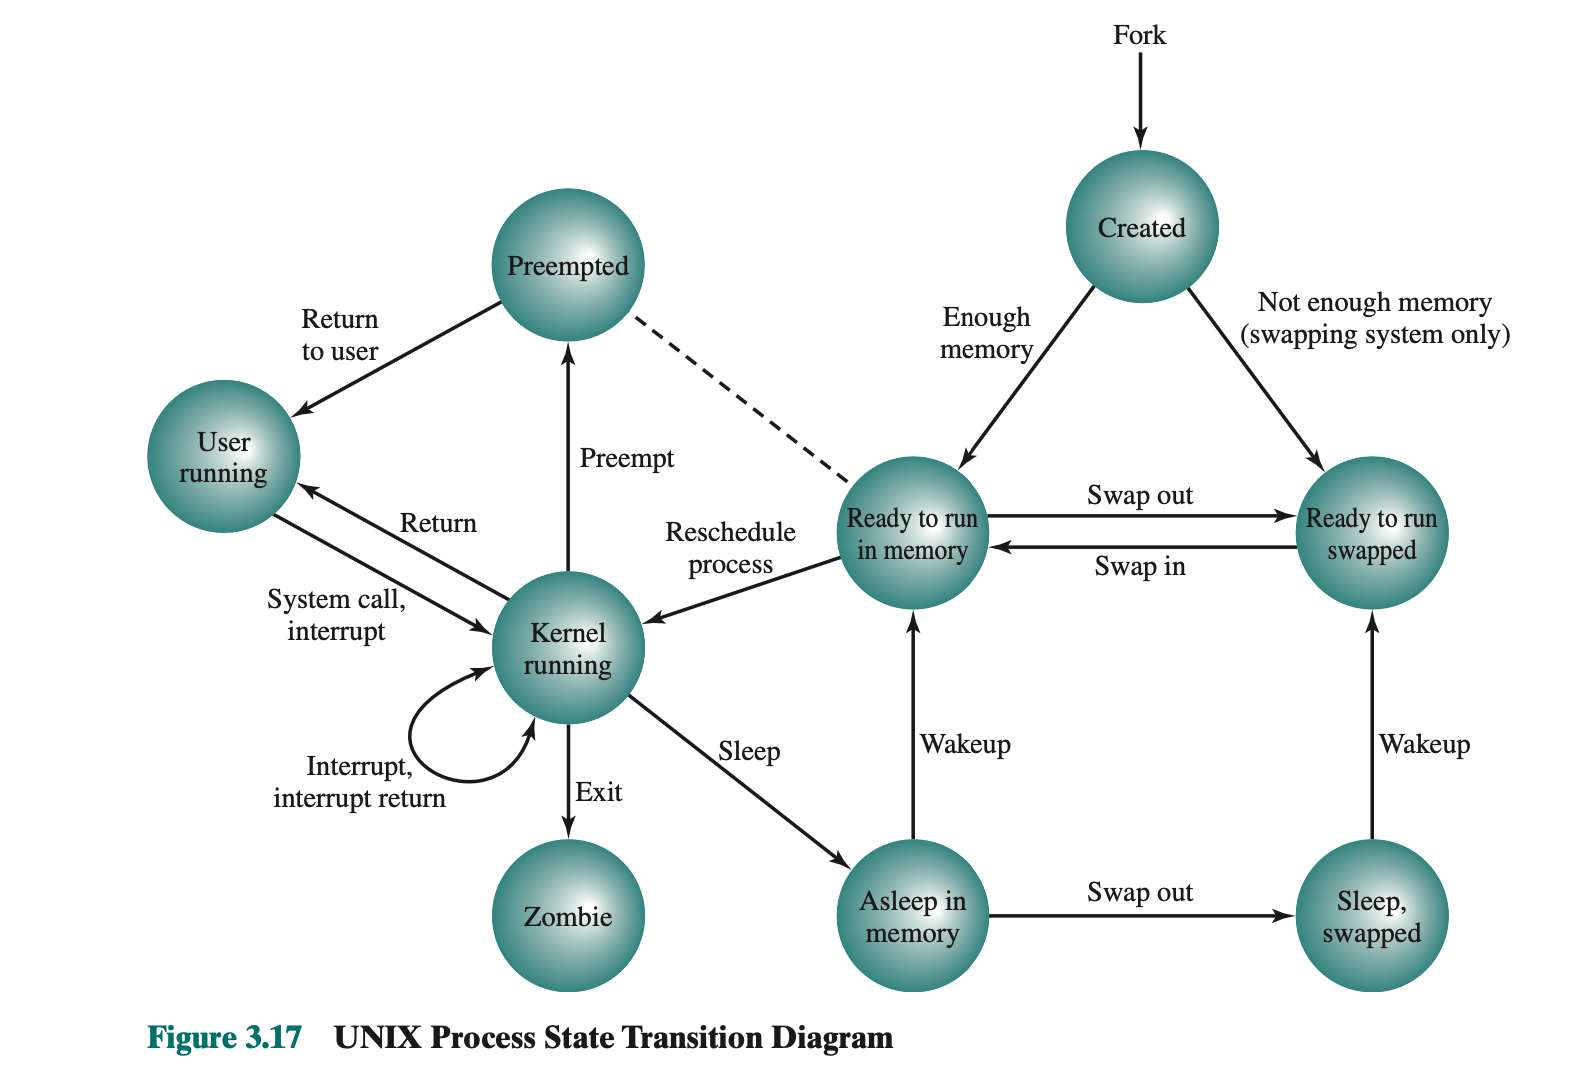
\includegraphics[width=0.8\textwidth]{img/2.3.1.3}
	\end{figure}


	\subsection{进程的数据描述}
	\subsubsection{进程控制块}
	操作系统程序为管理进程建立了一个管理数据结构——进程控制块(process control block, PCB)
	\begin{itemize}
		\item 它是进程存在的唯一标识,是操作系统用于记录和刻画进程状态及环境信息的数据结构
		\item 进程控制块包括进程执行时的情况,以及进程让出处理器之后所处的状态、断点等信息进程控制块应包含以下三类信息:
		\begin{itemize}
			\item 标识信息:用于存放唯一标识该进程的信息
			\begin{itemize}
				\item 系统分配的标识号
				\item 系统分配的进程组标识号
				\item 用户定义的进程名
				\item 用户定义的进程组名
			\end{itemize}
			\item 现场信息:用于存放该进程运行时的处理器现场信息
			\begin{itemize}
				\item 用户可见寄存器内容:数据寄存器、地址寄存器
				\item 控制与状态寄存器内容:PC、IR、PSW
				\item 栈指针内容:核心栈与用户栈指针
			\end{itemize}
			\item 控制信息:用于存放与管理、调度进程相关
			的信息
			\begin{itemize}
				\item 调度相关信息:状态、等待事件/原因、优先级
				\item 进程组成信息:代码/数据地址、外存映像地址
				\item 队列指引元:进程队列指针、父子兄弟进程指针
				\item 通信相关信息:消息队列、信号量、锁
				\item 进程特权信息:如内存访问权限、处理器特权
				\item 处理理器使用信息:占用的处理器、时间片、处理器使用时间/已执行总时间、记账信息
				\item 资源清单信息:如正占有的资源、已使用的资源
			\end{itemize}
		\end{itemize}
	\end{itemize}
	\begin{figure}[H]
		\centering
		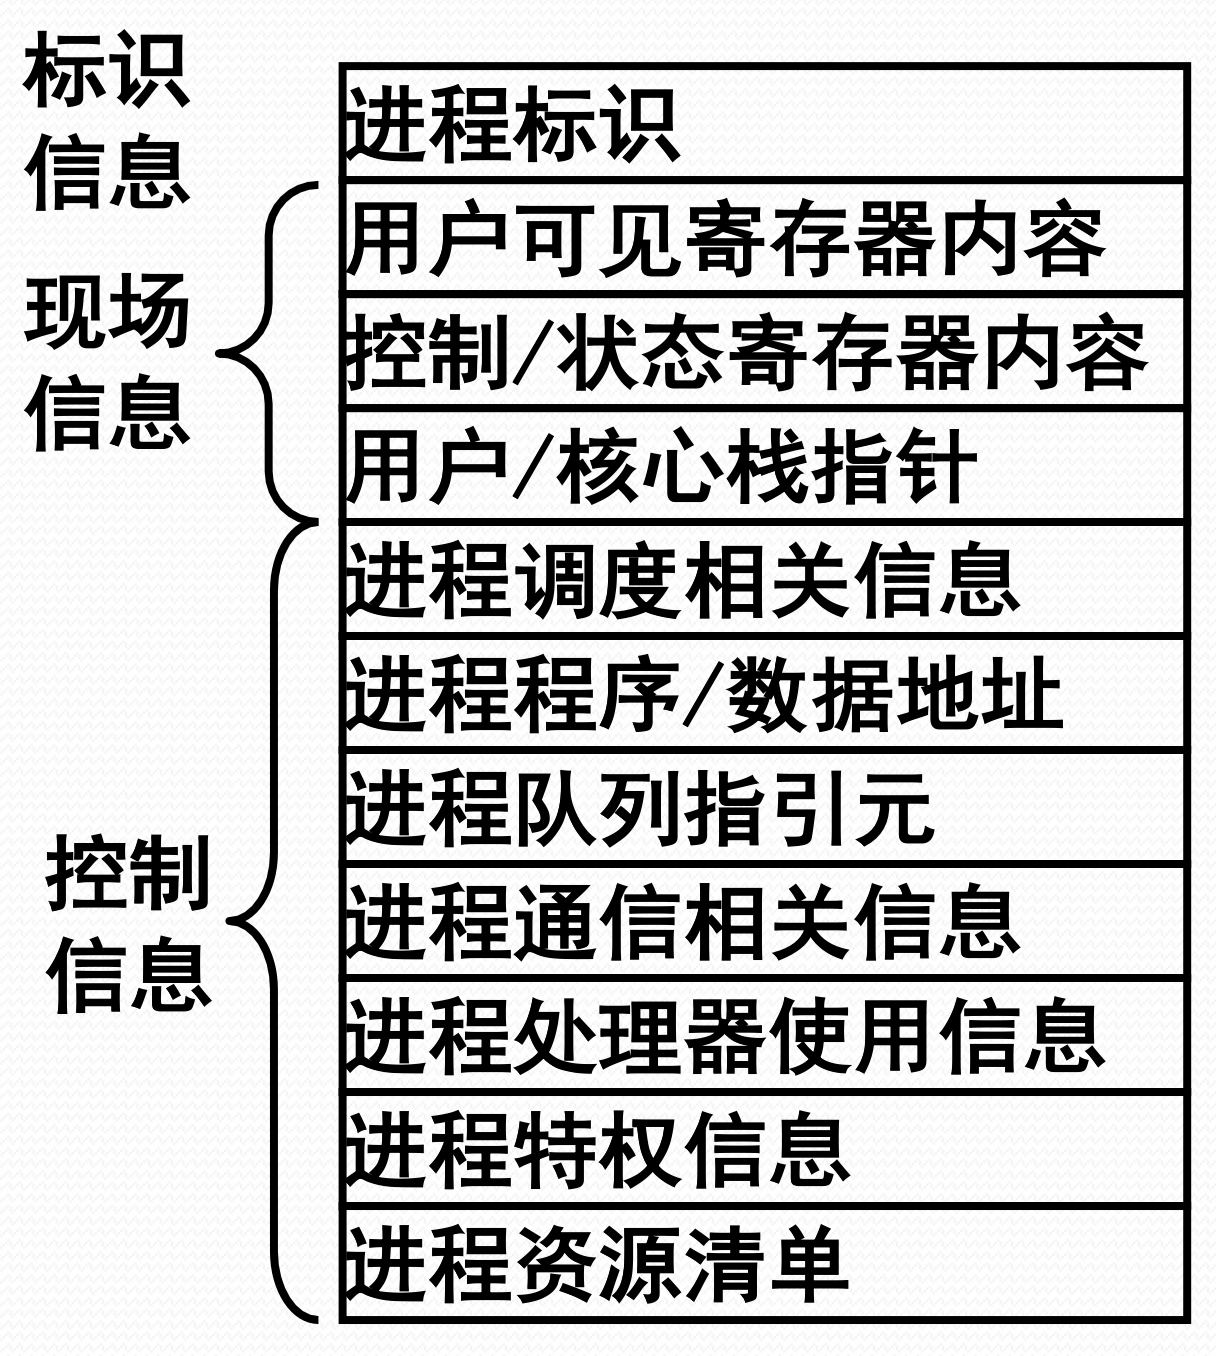
\includegraphics[width=0.4\textwidth]{img/2.3.2.1}
	\end{figure}


	\subsubsection{进程映像}
	进程映像是某一时刻进程的内容及其执行状态集合
	\begin{itemize}
		\item 进程控制块:每个进程捆绑一个,保存进程的标识信息、现场信息和控制信息。进程创建时创建进程控制块,进程撤销时回收进程控制块,与进程一一对应
		\item 进程程序块:进程执行的程序空间,规定进程一次运行所应完成的功能
		\item 进程数据块:进程处理的数据空间,是进程的私有地址空间,包括各类私有数据、处理函数的用户栈和可修改的程序
		\item 进程核心栈:每个进程捆绑一个,进程在内核模式下运行时使用的堆栈,中断或系统过程使用,保存函数调用的参数、局部变量和返回地址等
	\end{itemize}

	进程映像是内存级的物理实体,又称为进程的内存映像

	\begin{figure}[H]
		\centering
		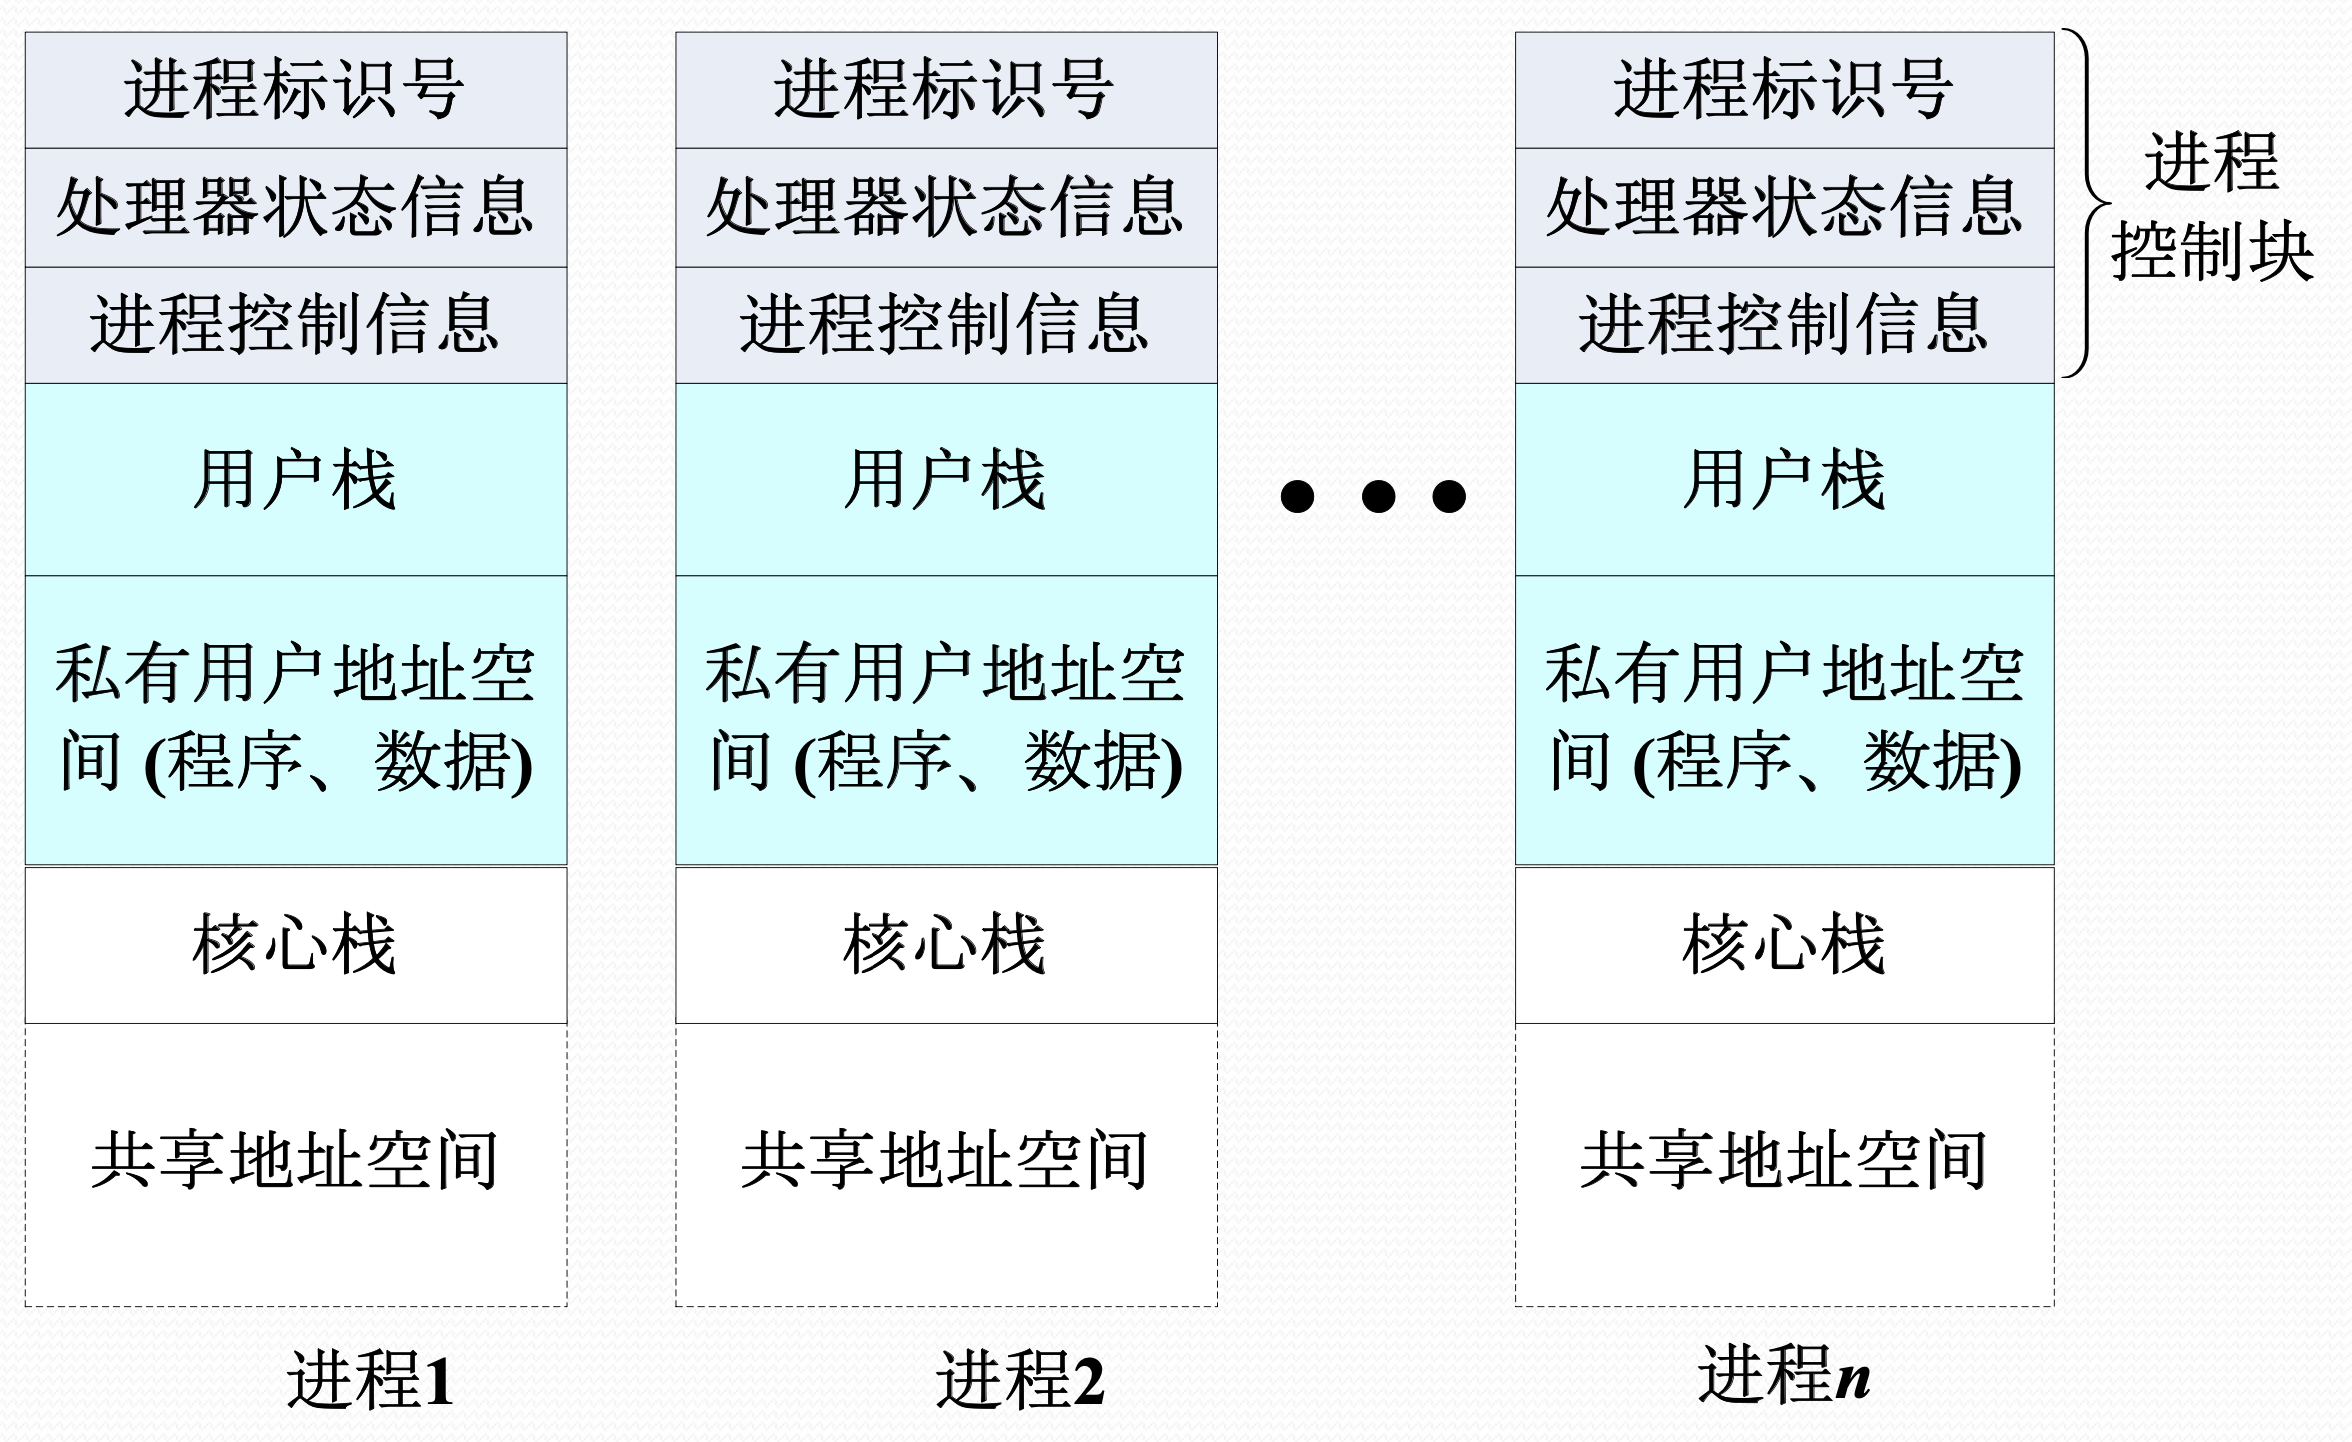
\includegraphics[width=0.7\textwidth]{img/2.3.2.2}
	\end{figure}


	\subsubsection{进程上下文}
	进程在系统中的存在和活动除了进程映像外,还需要环境的支撑,包括 CPU 现场和 Cache 中的执行信息

	操作系统中的进程物理实体和支持进程运行的环境合成进程上下文,由以下三部分组成:
	\begin{itemize}
		\item 用户级上下文:
		\begin{itemize}
			\item 用户程序块(可执行的机器指令序列)
			\item 用户数据区(进程可访问的信息)
			\item 用户栈(存放函数调用过程中的信息)
			\item 用户共享内存(进程通信使用的内存区)
			\item 对换至磁盘的分段或页面仍然是用户级上下文的组成部分
		\end{itemize}
		\item 寄存器上下文:
		\begin{itemize}
			\item 处理器状态寄存器(进程当前状态)
			\item 指令计数器(下一条该执行的指令地址)
			\item PSW/栈指针(指向用户栈或核心栈当前地址)
			\item 通用寄存器等
		\end{itemize}
		\item 系统级上下文
		\begin{itemize}
			\item 进程控制块(PCB,进程的状态)
			\item 内存区管理信息(进程页表或段表)
			\item 核心栈等(进程内核态运行时的工作区)
		\end{itemize}
	\end{itemize}
	进程上下文刻画了进程的执行情况


	\subsection{进程管理的实现}
	关键的进程管理软件包括:
	\begin{itemize}
		\item 系统调用/中断/异常处理程序
		\item 队列管理模块
		\item 进程控制程序
		\item 进程调度程序(独立进程居多)
		\item 进程通信程序(多个程序包)
		\item 终端登录与作业控制程序、性能监控程序、审计程序等外围程序
	\end{itemize}

	\subsubsection{队列管理程序}
	队列管理模块是操作系统实现进程管理的核心模块
	\begin{itemize}
		\item 操作系统将进程组织成若干个队列进行管理,新建的进程一般进入就绪队列
		\item 操作作系统根据调度需求可以有一个或几个就绪进程队列,当处理器空闲时,非空的最高优先级就绪队列中的进程就会占有处理器运行
		\item 当占有处理器运行的进程出现等待事件时,它就会进入等待事件队列;由于等待事件是多种多样的,所以操作系统必然维护有多个事件等待队列
		\item 等待事件结束后就会按照某种规则回到某一个就绪队列
		\item 当出现了更高优先级的抢占式进程,或者出现时间片到的现象时,操作系统会强迫处于运行态的进程让出处理器,进入就绪队列,然后让抢占进程或就绪进程队列中排队的进程去占有处理器运行
		\item 运行态的进程最终会在处理器上通过执行一条系统调用进入结束终止的完成状态
	\end{itemize}

	\begin{figure}[H]
		\centering
		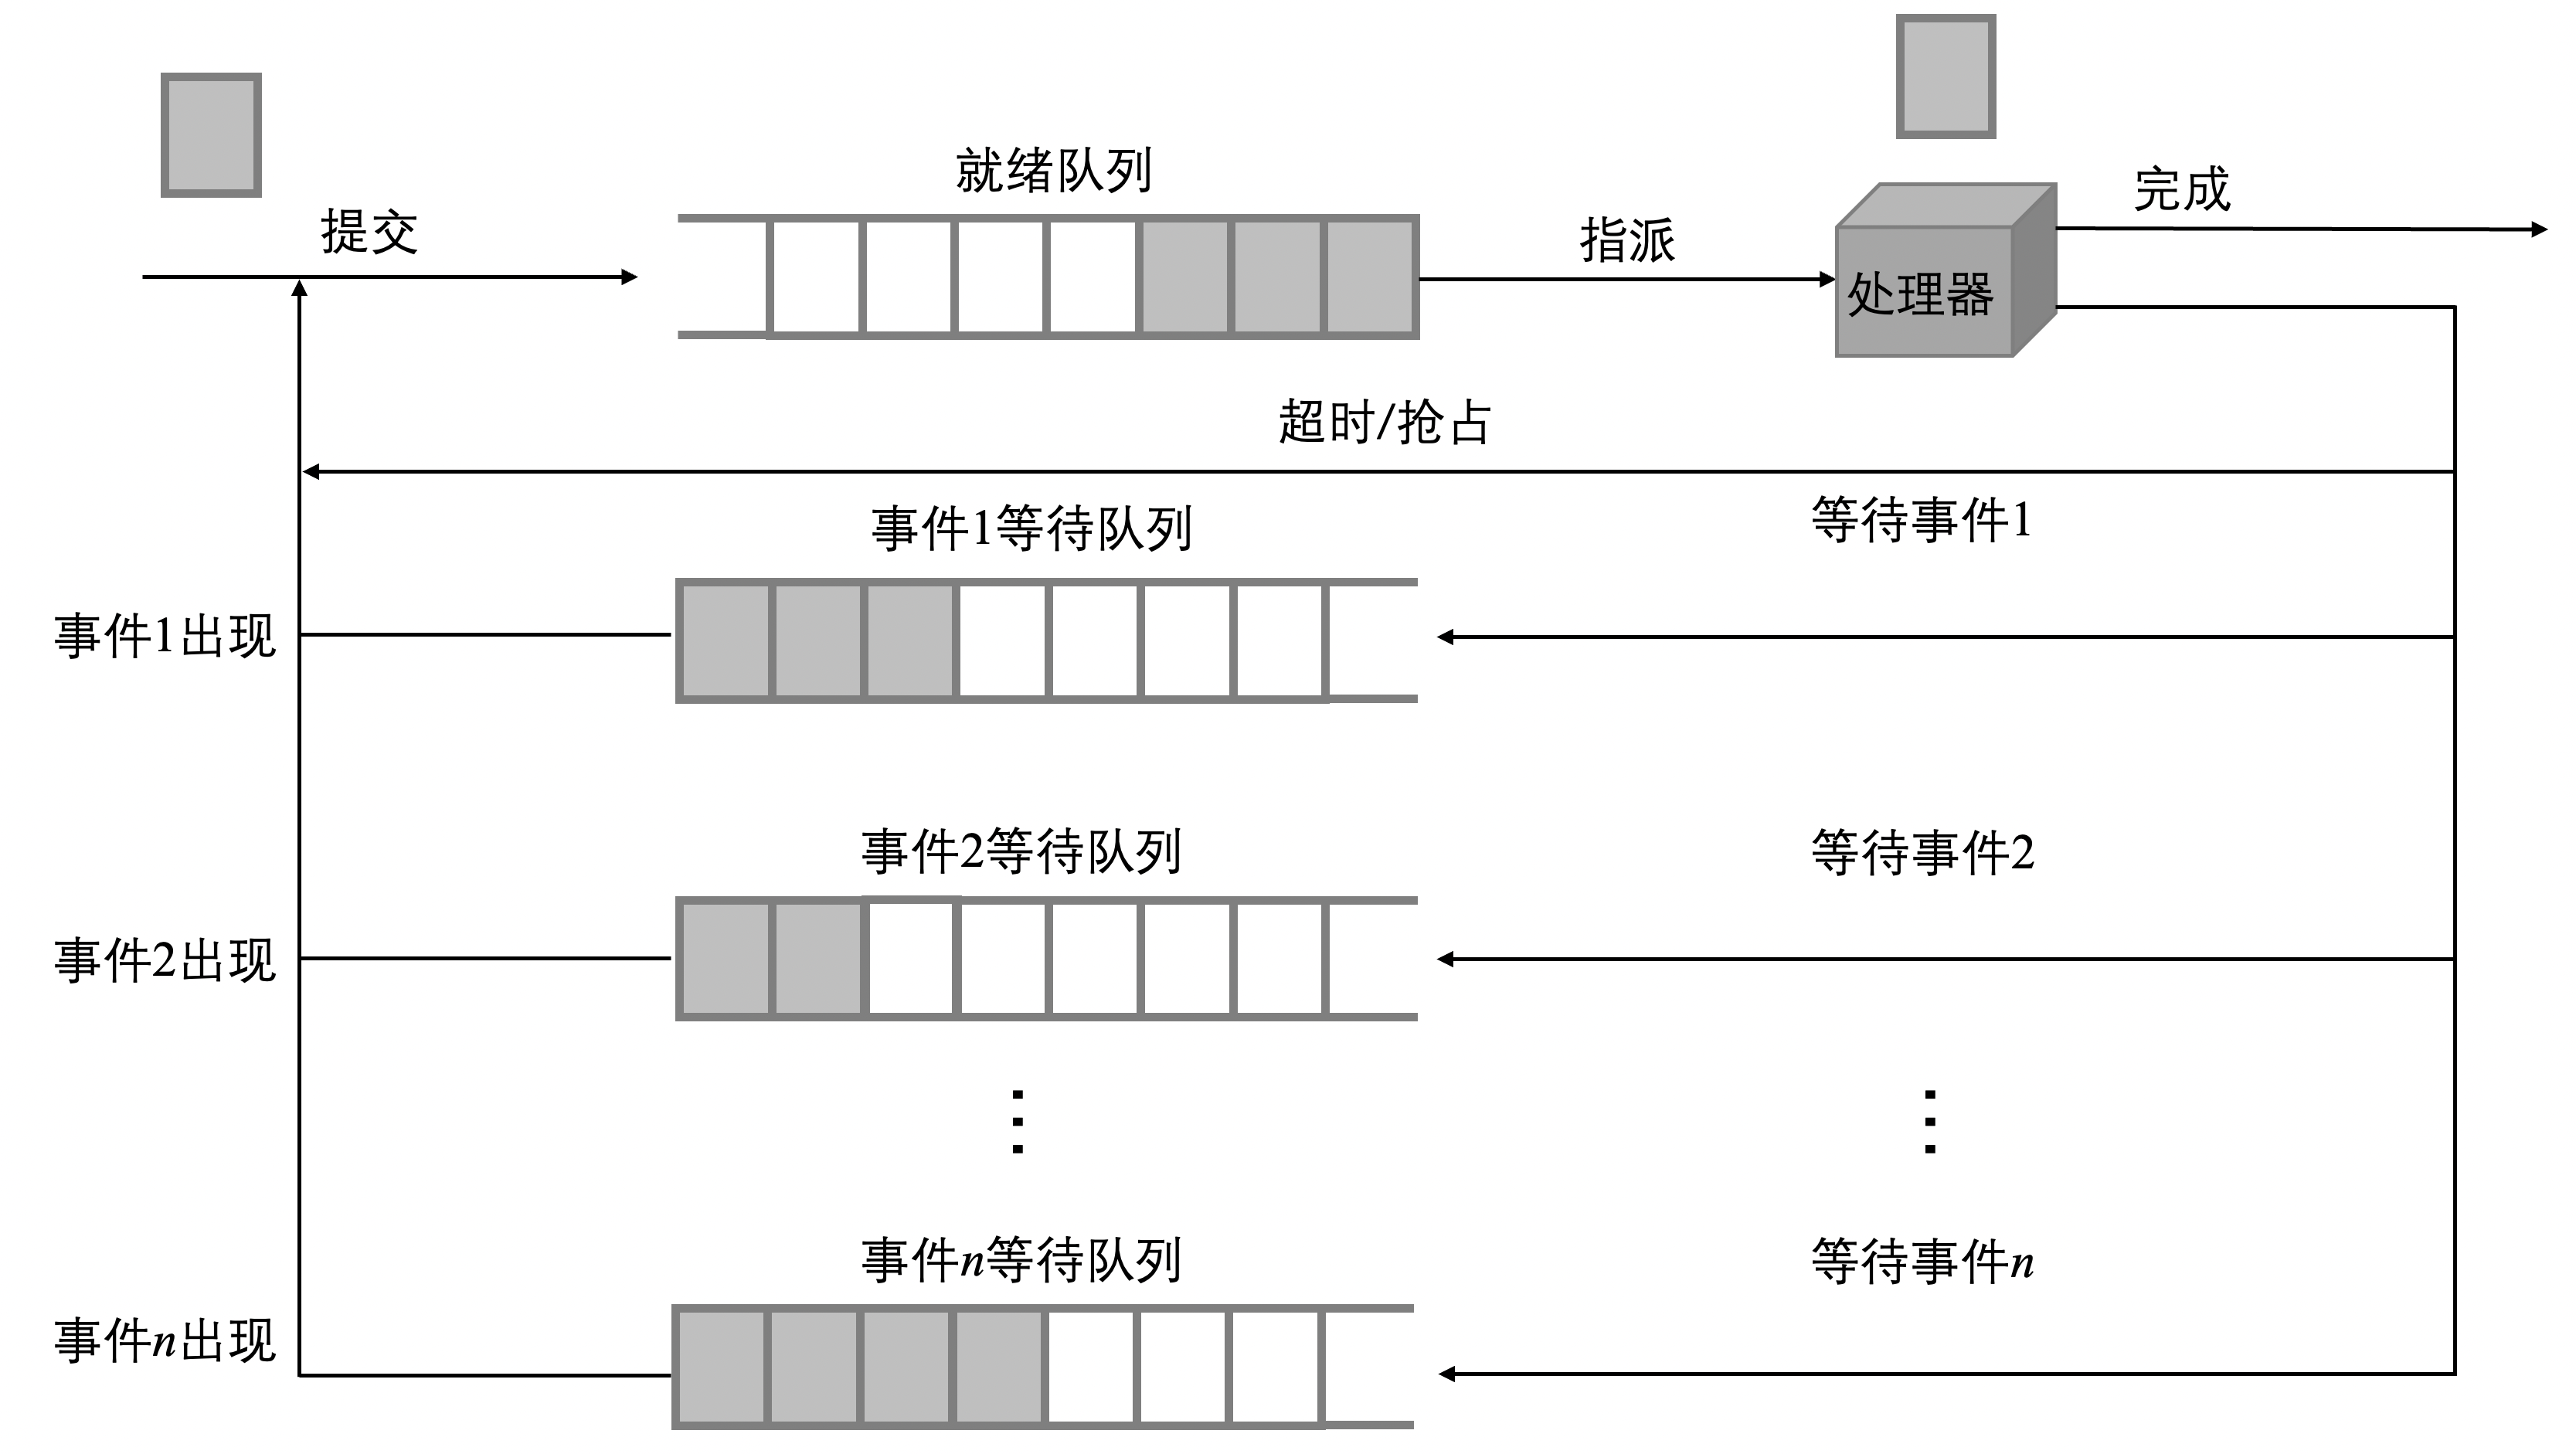
\includegraphics[width=0.85\textwidth]{img/2.3.3.1.1}
	\end{figure}
	进程队列的组织分为链接方式和索引方式两种组织方式
	\begin{figure}[H]
		\centering
		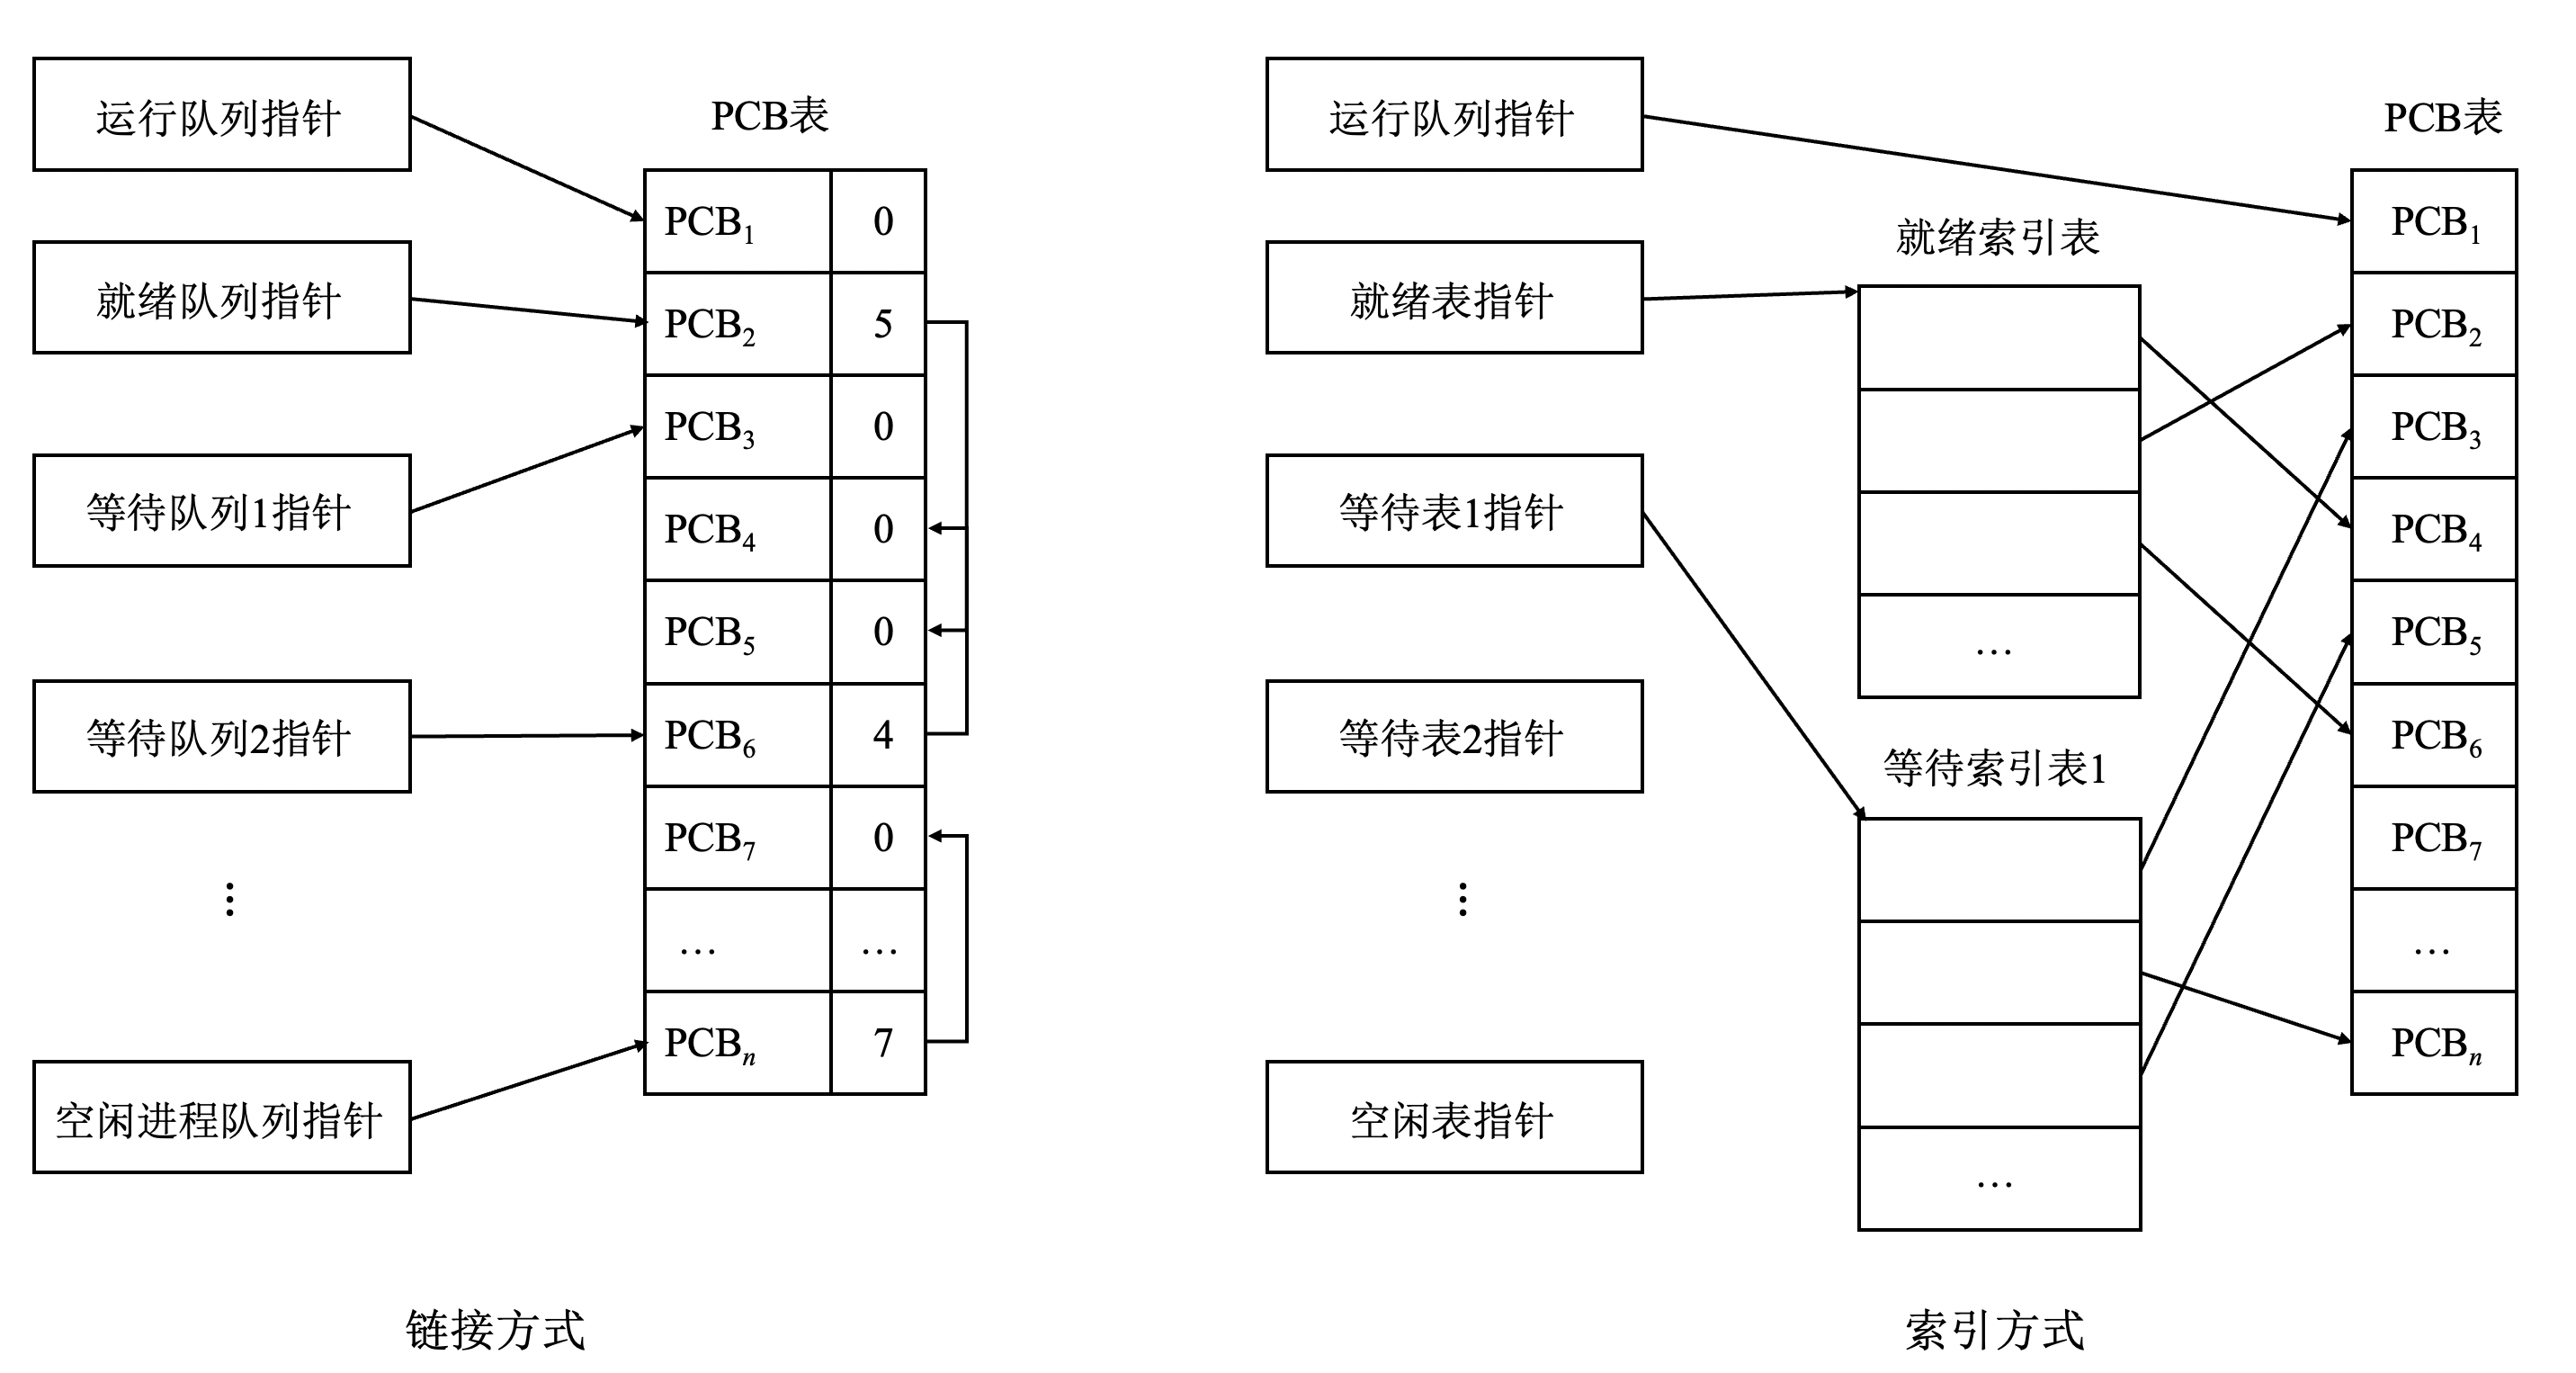
\includegraphics[width=0.85\textwidth]{img/2.3.3.1.2}
	\end{figure}


	\subsubsection{进程控制程序}
	\begin{itemize}
		\item 进程控制程序包括进程的创建、进程的撤销、进程的阻塞、进程的唤醒、进程的挂起、进程的激活,以及进程特权的修改等操作
		\item 它们往往被抽象成一组系统调用,在实现上是一个处理的流程
		\item 进程控制需要对操作系统的核心数据结构进行操作,应采用\textbf{原语}来实现进程控制中的核心操作
		\begin{itemize}
			\item 原语是由若干条指令构成的完成某种特点功能的程序,执行上具有不可分割性,这样能保证对核心资源访问的正确性
			\item 原语实现的具体办法是进入原语前关闭中断,在退出原语前开放中断
		\end{itemize}
	\end{itemize}
	
	部分进程管理原语
	\begin{itemize}
		\item \textbf{进程创建}:
		\begin{itemize}
			\item 操作系统初始启动时会创建承担系统资源分配和控制管理的一些系统进程,同时会创建一个所有用户集成的祖先,其他用户进程实在用户程序被提价与选中运行时被创建的
			\item 操作系统通常将创建关系通过父子进程的关系来表示
			\item 创建原语:进程表加一项、申请 PCB 并初始化、生成唯一进程标识、建立进程映像、分配各种资源、移入就绪队列、通知操作系统某些模块
		\end{itemize}
		\item \textbf{进程撤销}:
		\begin{itemize}
			\item 完成特定工作或出现严重错误后需要撤销,分为正常撤销和非正常撤销
			\item 产生原因:运行结束、执行非法指令、用户态执行特权指令、时间配额到、等待时间超时、越界错误、共享内存区非法使用、程序性故障等
			\item 撤销原语:从队列中移除、归还资源、撤销标识、回收 PCB、移除进程表项
		\end{itemize}
		\item \textbf{进程阻塞}:
		\begin{itemize}
			\item 使得进程让出处理器转而等待一个事件,比如等待资源等,阻塞是同步时间
			\item 阻塞原语:保存现场信息、修改 PCB、移入等待队列、调度其他进程执行
		\end{itemize}
		\item \textbf{进程唤醒}:
		\begin{itemize}
			\item 等待时间完成时产生一个中断,激活操作系统,在系统的控制下将被阻塞进程唤醒
			\item 唤醒原语:等待队列中移出、修改 PCB、移入就绪队列(该进程优先级高于运行进程触发抢占)
		\end{itemize}
		\item \textbf{进程挂起}:
		\begin{itemize}
			\item 出现引起挂起的事件时,系统或进程会利用挂起原语把指定进程或处于等待态的进程挂起
			\item 挂起原语:修改状态并出入相关队列、收回内存等资源送至对换区
			\item 挂起原语可以由进程自己或其他进程调起
		\end{itemize}
		\item\textbf{进程激活}:
		\begin{itemize}
			\item 当系统资源尤其是内存资源充裕或请求激活进程时,系统或相关进程会调用激活原语将指定进程激活
			\item 激活原语:分配内存,修改状态并出入相关队列
			\item 激活原语只能由其他进程调用
		\end{itemize}
	\end{itemize}

	\subsection{进程切换与模式切换}
	\subsubsection{进程上下文切换}
	进程切换指从正在运行的进程中收回处理器,让待运行进程来占有处理器运行

	进程切换必然发生在内核态而非用户态

	进程切换实质上就是被中断运行进程与待运行进程的上下文切换,处理过程是:
	\begin{itemize}
		\item (中断/异常等触发)正向模式切换并压入 PSW/PC
		\item 保存被中断进程的现场信息
		\item 处理具体中断/异常
		\item 把被中断进程的系统堆栈指针 SP 值保存到 PCB
		\item 调整被中断进程的 PCB 信息,如进程状态
		\item 把被中断进程的 PCB 加入相关队列
		\item 选择下一个占用 CPU 运行的进程
		\item 修改被选中进程的 PCB 信息,如进程状态
		\item 设置被选中进程的地址空间,恢复存储管理信息
		\item 恢复被选中进程的 SP 值到处理器寄存器 SP
		\item 恢复被选中进程的现场信息进入处理器
		\item (中断返回指令触发)逆向模式转换并弹出 PSW/PC
	\end{itemize}

	\subsubsection{进程上下文的切换时机}
	进程切换一定发生在\textbf{中断/异常/系统调用处理}过程中,常见的情况是:
	\begin{itemize}
		\item 阻塞式系统调用、虚拟地址异常导致被中断进程进入等待态
		\item 时间片中断、I/O 中断后发现更高优先级进程,导致被中断进程转入就绪态
		\item 终止用系统调用、不能继续执行的异常导致被中断进程进入终止态
	\end{itemize}
	内核不能执行调度和切换的情况:
	\begin{itemize}
		\item 内核正在处理中断的过程中
		\item 进程运行在内核临界区
		\item 内核处在需要屏蔽中断的原子操作过程中
	\end{itemize}
	如果在上述过程中产生引起调度的条件,不能马上进行调度和切换,系统将采用置请求调度标志,延迟到敏感性操作完成后才进行


	\subsubsection{处理器模式切换}
	进程切换必须在操作系统内核模式下完成,这就需要模式切换

	模式切换又称处理器状态切换,包括:
	\begin{itemize}
		\item 用户模式到内核模式(正向模式切换)
		\begin{itemize}
			\item 由中断/异常/系统调用中断用户进程执行而触发
			\item 中断装置完成正向模式切换,包括:
			\begin{itemize}
				\item 处理器模式转为内核模式 
				\item 保存当前进程的 PC/PSW 值到核心栈
				\item 转向中断/异常/系统调用处理程序
			\end{itemize}
		\end{itemize}
		\item 内核模式到用户模式(逆向模式切换)
		\begin{itemize}
			\item 操作系统执行中断返回指令将控制权交还用户进程而触发
			\item 中断返回指令完成逆向模式转换,包括:
			\begin{itemize}
				\item 从待运行进程核心栈中弹出 PSW/PC 值
				\item 处理器模式转为用户模式
			\end{itemize}
		\end{itemize}
	\end{itemize}

	一些中断/异常不会引起进程状态转换,不会引起进程切换,只是在处理完成后把控制权交回给被中断进程,处理流程是:
	\begin{itemize}
		\item (中断/异常触发)正向模式切换压入 PSW/PC
		\item 保存被中断进程的现场信息
		\item 处理中断/异常
		\item 恢复被中断进程的现场信息
		\item (中断返回指令触发)逆向模式转换弹出 PSW/PC
	\end{itemize}
	\begin{figure}[H]
		\centering
		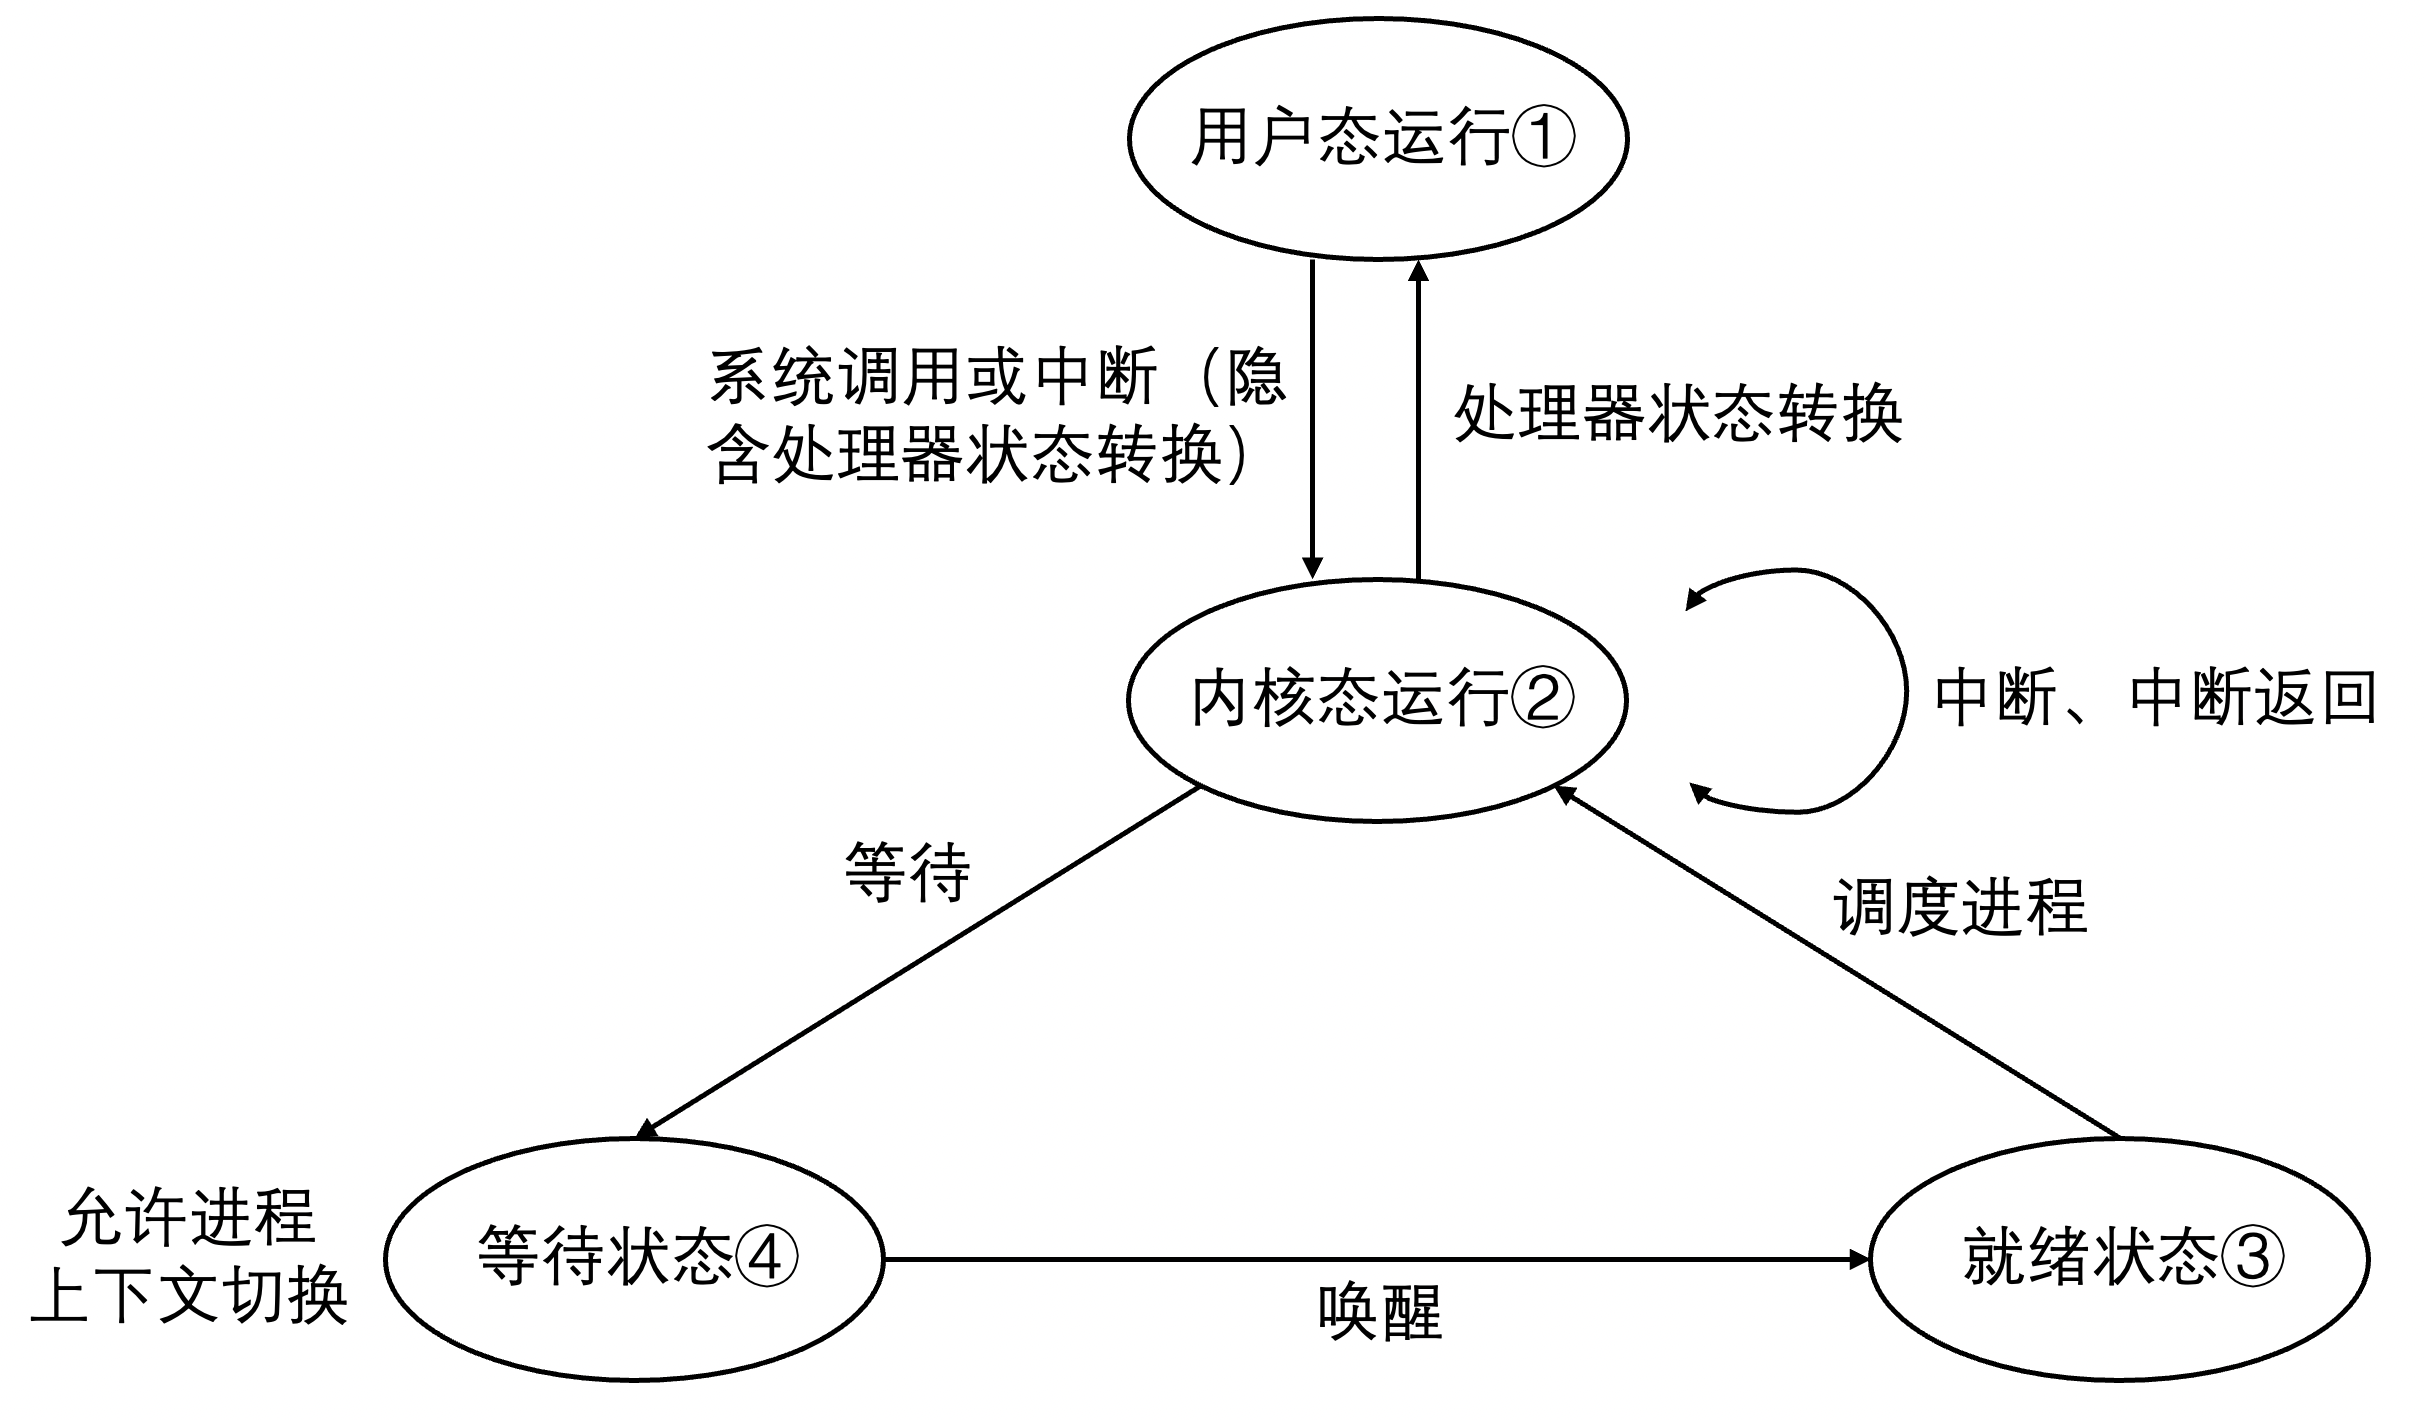
\includegraphics[width=0.55\textwidth]{img/2.3.4.3}
	\end{figure}


	\section{多线程技术}
	\subsection{多线程环境概述}
	\subsubsection{多线程技术的提出}
	单线程结构进程在并发程序设计上存在的问题
	\begin{itemize}
		\item 进程切换开销大
		\item 进程通信开销大
		\item 限制了进程并发的粒度
		\item 降低了并行计算的效率
	\end{itemize}
	\begin{figure}[H]
		\centering
		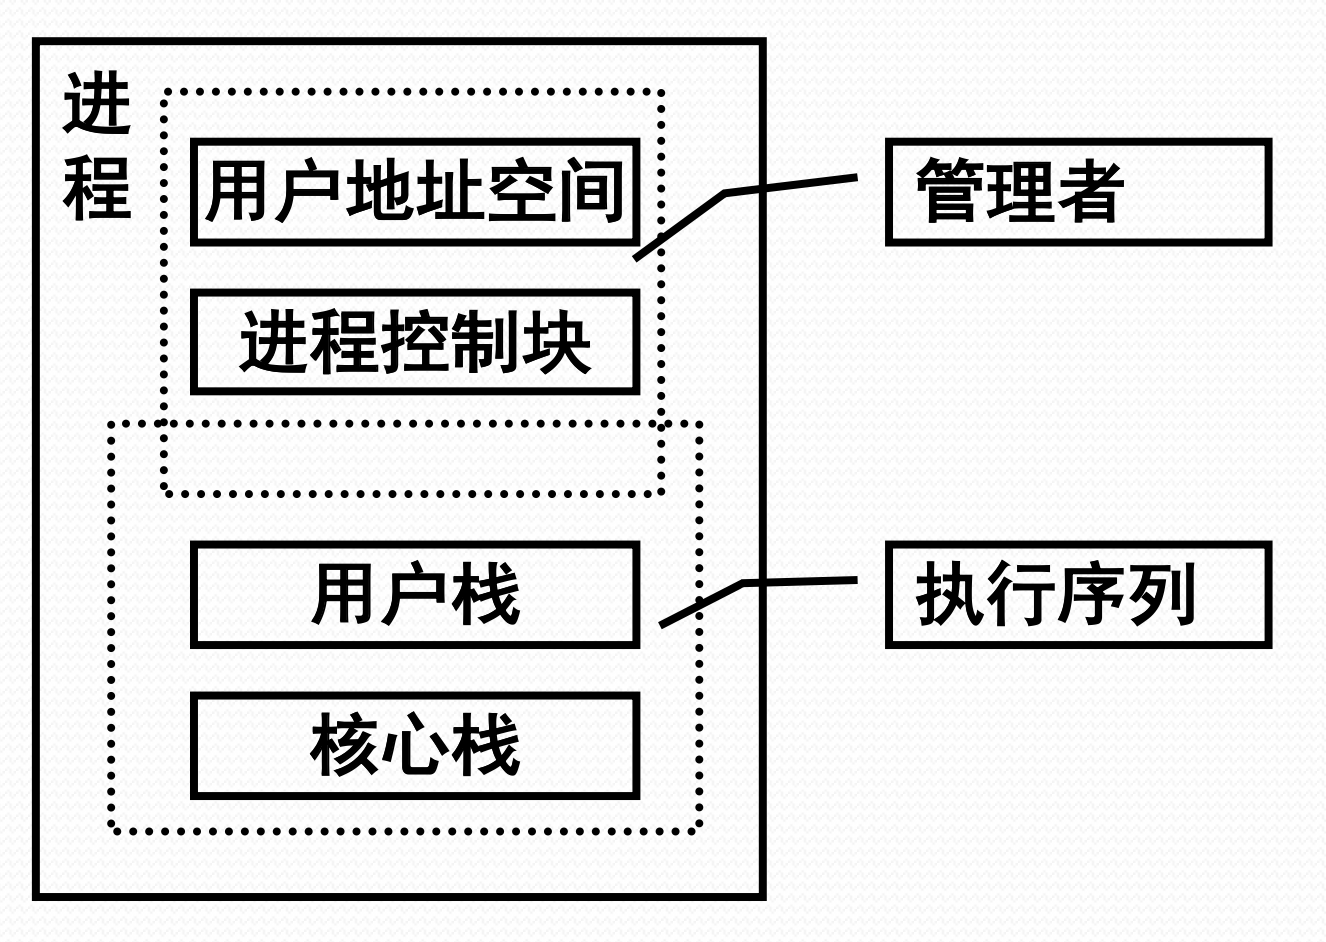
\includegraphics[width=0.4\textwidth]{img/2.4.1.1}
	\end{figure}

	解决上述问题的思路
	\begin{itemize}
		\item 把进程的两项功能,即“独立分配资源”与“被调度分派执行”分离开来
		\item 进程作为系统资源分配和保护的独立单位,不需要频繁地切换
		\item 线程作为系统调度和分派的基本单位,能轻装运行,会被频繁地调度和切换
		\item 线程的出现会减少进程并发执行所付出的时空开销,使得并发粒度更细、并发性更好
	\end{itemize}


	\subsubsection{多线程环境下的进程}
	\begin{figure}[H]
		\centering
		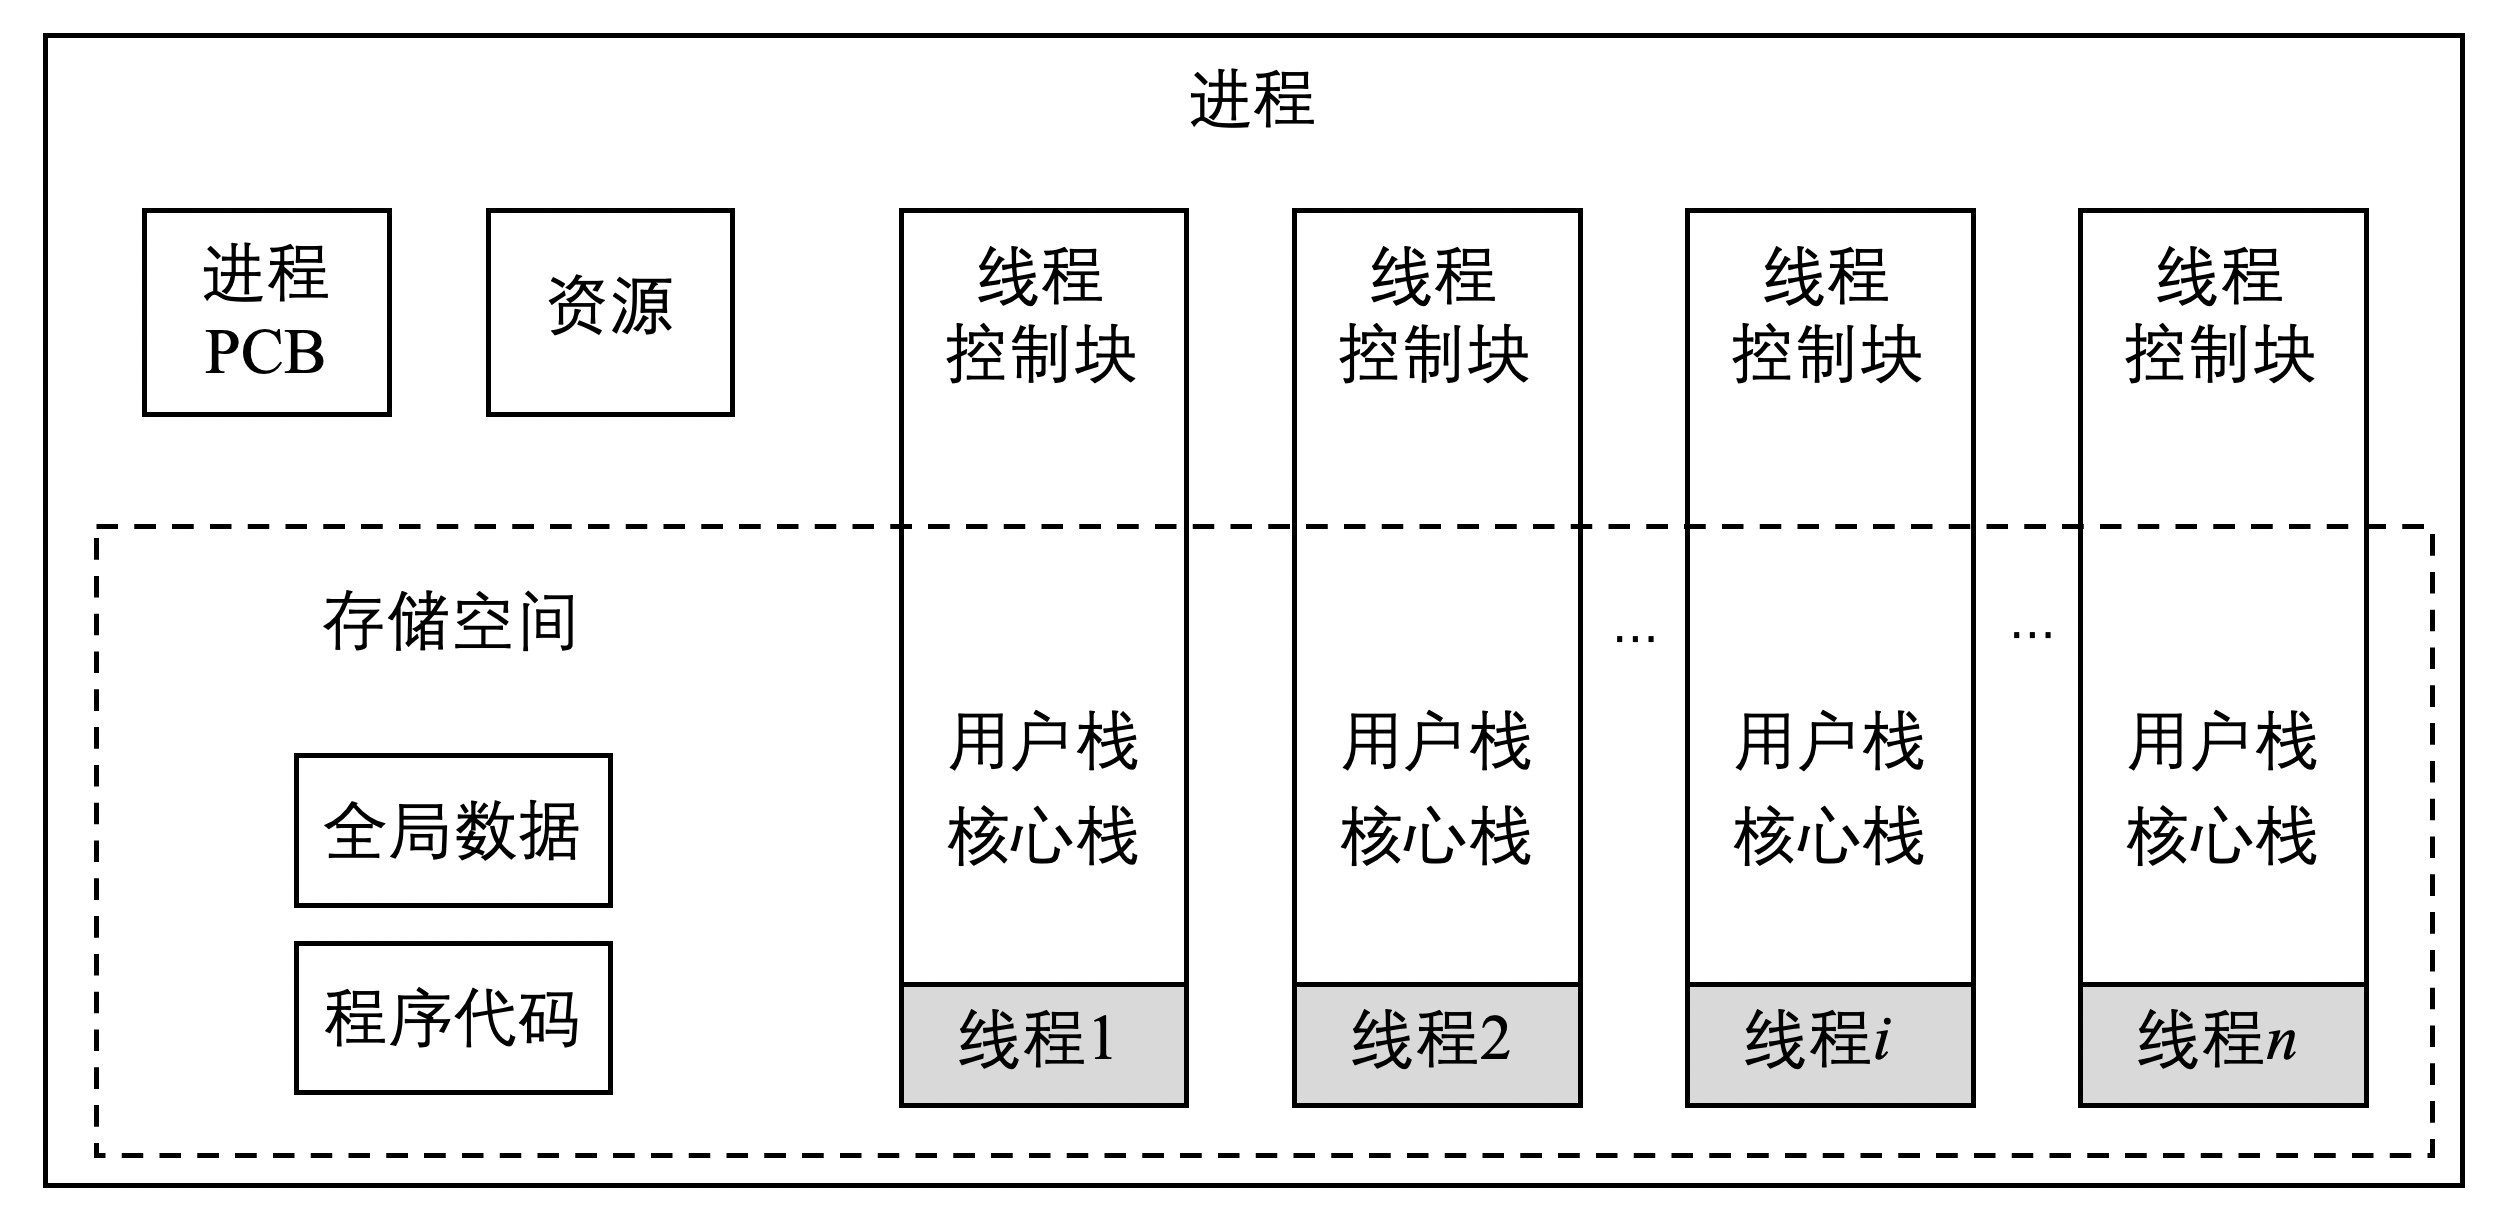
\includegraphics[width=0.65\textwidth]{img/2.4.1.2}
	\end{figure}

	在多线程环境中,进程是操作系统中进行保护和资源分配的独立单位。具有:
	\begin{itemize}
		\item 用来容纳进程映像的虚拟地址空间
		\item 对进程、文件和设备的存取保护机制
	\end{itemize}

	线程是进程的一条执行路径,是调度的基本单位,同一个进程中的所有线程共享进程获得的主存空间和资源。它具有:
	\begin{itemize}
		\item 线程执行状态
		\item 受保护的线程上下文,当线程不运行时,用于存储现场信息
		\item 独立的程序指令计数器
		\item 执行堆栈
		\item 容纳局部变量的静态存储器
	\end{itemize}

	多线程环境下线程的状态与调度

	\begin{itemize}
		\item 线程状态有运行、就绪和等待和终止
		\begin{itemize}
			\item 没有挂起状态是因为挂起和资源有关,由于线程不是资源拥有单位,所以挂起对线程来说是没有意义的
		\end{itemize}
		\item 与线程状态变化有关的线程操作有:孵化、封锁、活化、剥夺、指派、结束
		\item 操作系统感知线程环境下:
		\begin{itemize}
			\item 处理器调度的对象是线程
			\item 线程的存在、状态等都需要被操作系统内核感知到,进程没有三状态,或者说只有挂起状态
		\end{itemize}
		\item 操作系统不感知线程环境下:
		\begin{itemize}
			\item 处理器调度的单位仍然是进程
			\item 用户空间中的用户调度程序调度线程,内核不参加线程调度
		\end{itemize}
	\end{itemize}


	\subsubsection{多线程技术的优点与应用}
	并发多线程程序设计的优点
	\begin{itemize}
		\item 快速线程切换
		\item 减少(系统)管理开销
		\item (线程)通信易于实现
		\item 并行程度提高
		\item 节省内存空间
	\end{itemize}

	多线程技术的应用
	\begin{itemize}
		\item 前台和后台工作
		\item C/S 应用模式
		\item 加快执行速度
		\item 设计用户接口
	\end{itemize}


	\subsection{内核级线程与用户级线程}
	多线程的实现分为三类
	\begin{itemize}
		\item 内核级线程(kernel level thread, KLT),如 Windows 2003
		\item 用户级线程(user level thread, ULT),如 Java 线程库
		\item 混合方式,同时支持 ULT 和 KLT 两种线程,如 Solaris
	\end{itemize}

	\subsubsection{内核级线程}
	内核级线程是指线程管理工作由操作系统内核完成,并提供线程应用程序接口来使用线程

	内核需要为进程及进程中的单个线程维护现场信息,所以应在内核空间中建立和维护进程控制块及线程控制块(TCB)

	处理器调度以线程为单位,即内核的处理器调度程序直接选中某个就绪的线程

	\begin{figure}[H]
		\centering
		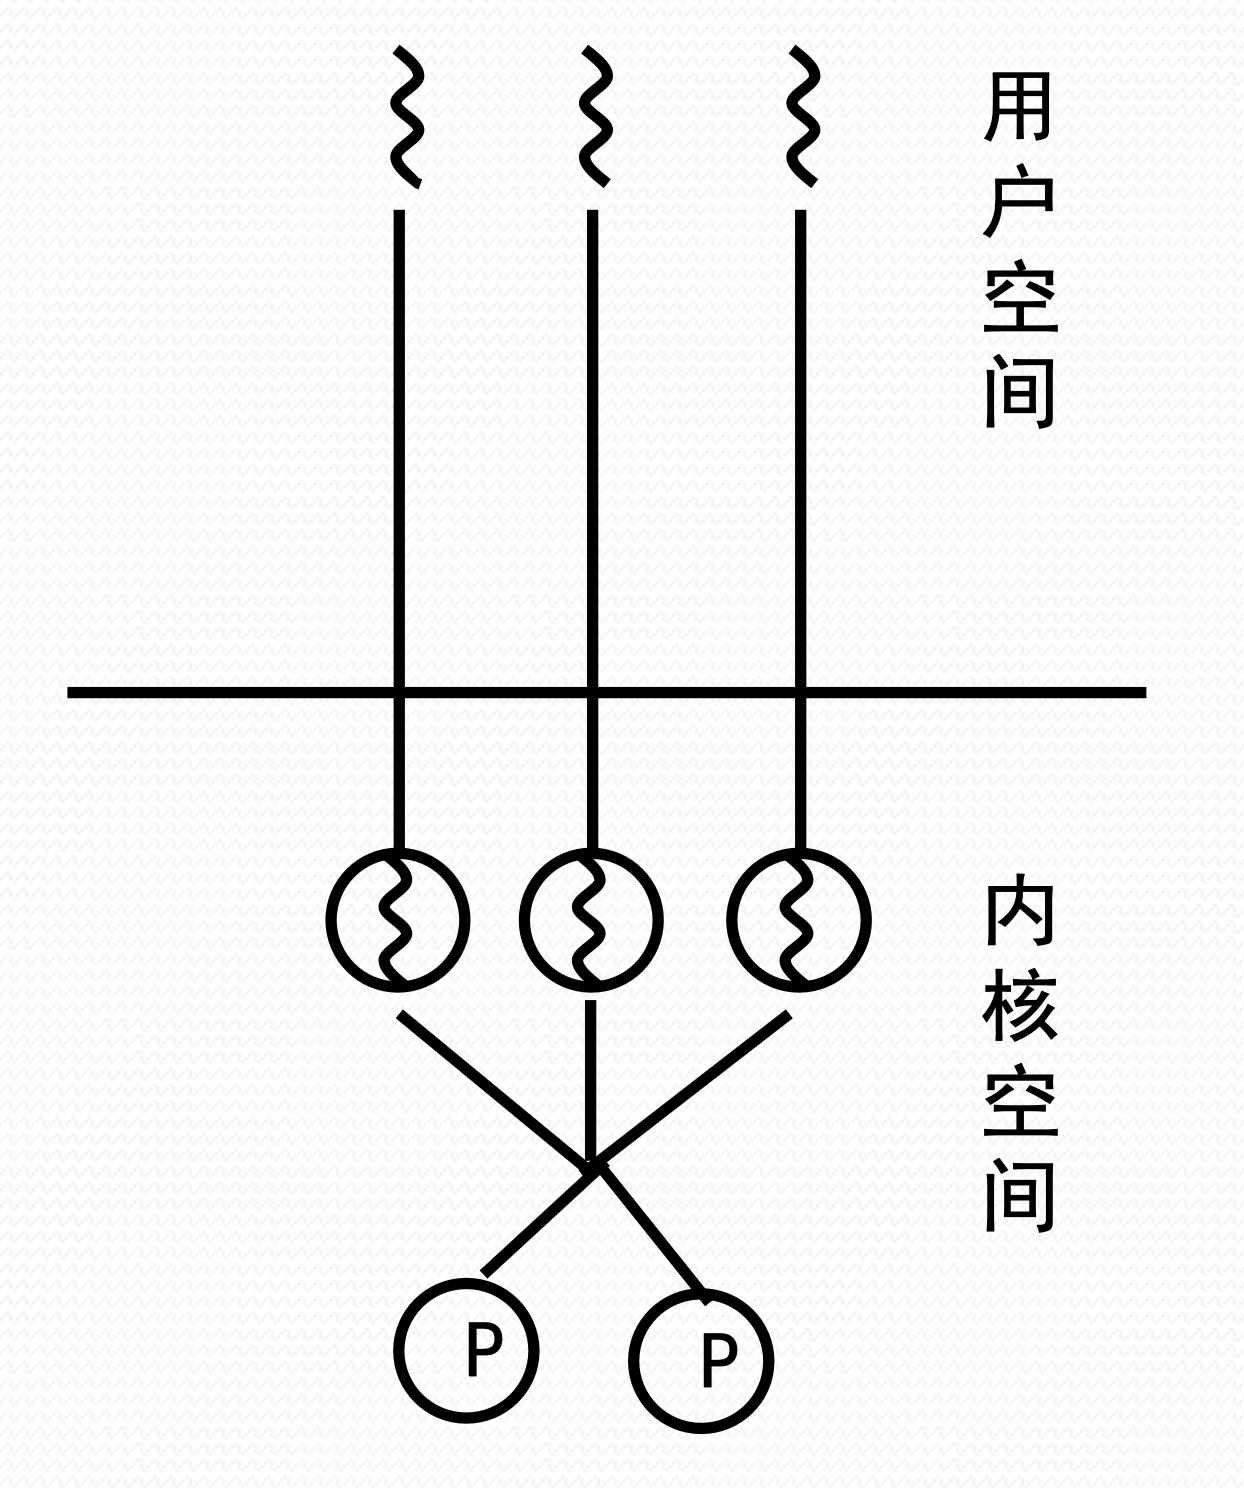
\includegraphics[width=0.3\textwidth]{img/2.4.2.1}
	\end{figure}

	内核级线程的特点:
	\begin{itemize}
		\item 进程中的一个线程被阻塞了,内核能调度同一进程的其它线程占有处理器运行
		\item 多处理器环境中,内核能同时调度同一进程中多个线程并行执行
		\item 内核自身也可用多线程技术实现,能提高操作系统的执行速度和效率
		\item 应用程序线程在用户态运行,线程调度和管理在内核实现,在同一进程中,控制权从一个线程传送到另一个线程时需要模式切换,系统开销较大
	\end{itemize}

	\subsubsection{用户级线程}
	用户级线程是指线程管理工作由应用程序来做,在用户空间内实现,内核不知道线程的存在

	应用程序需通过线程库进行程序设计,再与线程库连接后运行来实现多线程
	\begin{itemize}
		\item 线程库是一个用户级线程管理的例行程序包,主要功能有线程的创建、调度、管理等
		\item 在这种情况下,线程库是线程的运行支撑环境
	\end{itemize}
	\begin{figure}[H]
		\centering
		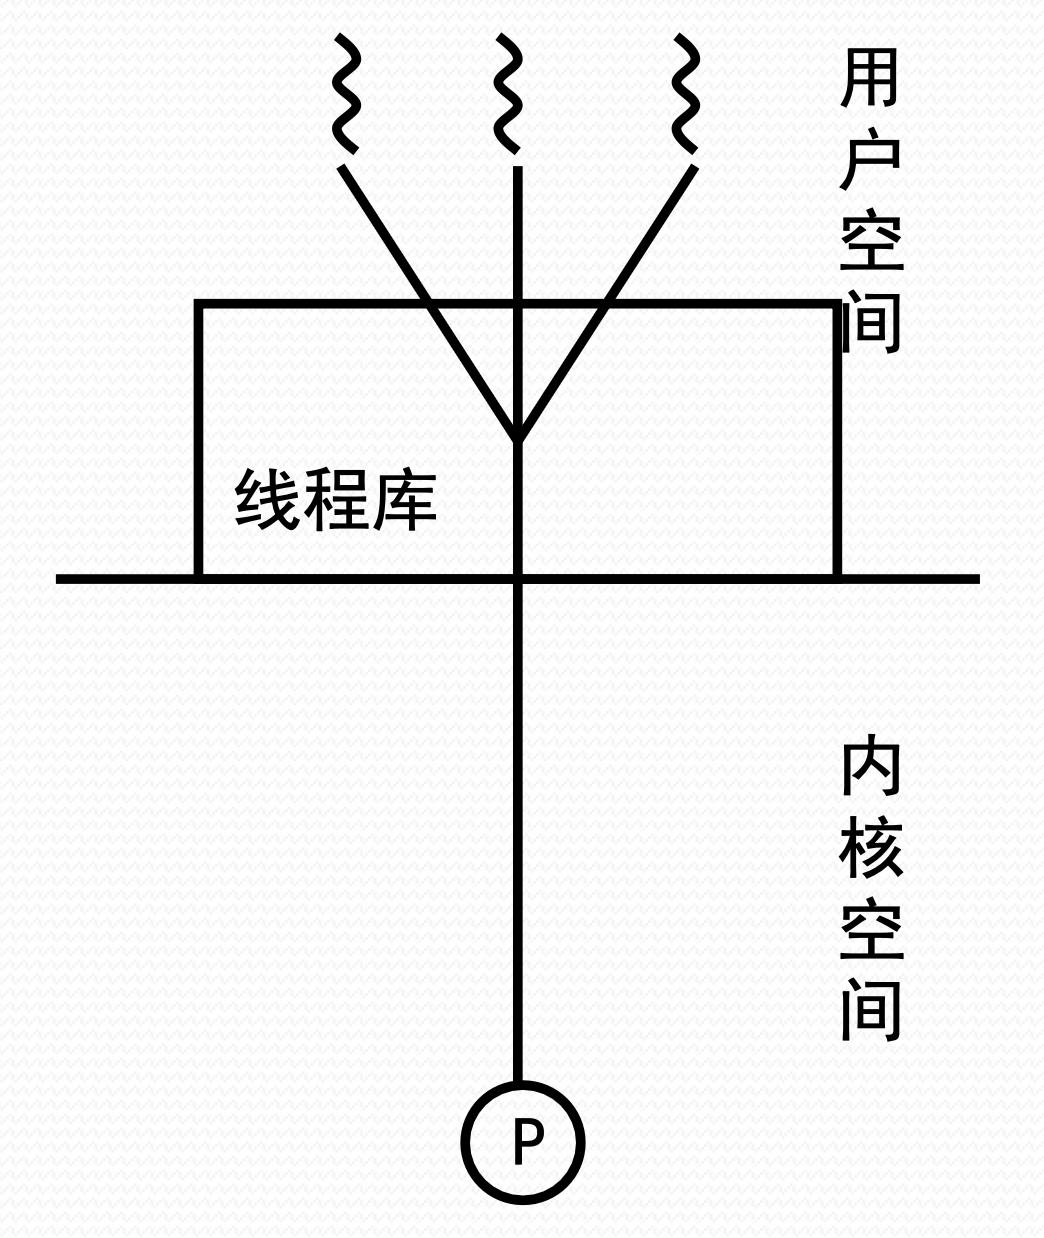
\includegraphics[width=0.3\textwidth]{img/2.4.2.2}
	\end{figure}

	用户级线程的特点:
	\begin{itemize}
		\item 所有线程管理数据结构均在进程的用户空间中,线程切换不需要内核模式,能节省模式切换开销和内核的宝贵资源
		\item 允许进程按应用特定需要选择调度算法,甚至根据应用需求裁剪调度算法
		\item 能运行在任何操作系统上,内核在支持 ULT 方面不需要做任何工作
		\item 不能利用多处理器的优点,操作系统调度进程, 仅有一个 ULT 能执行
		\item 一个 ULT 的阻塞将引起整个进程的阻塞
	\end{itemize}

	为了解决 ULT 的缺点,提出了 Jacketing 技术
	\begin{itemize}
		\item 把阻塞式系统调用改造成非阻塞式的
		\item 当线程陷入系统调用时,执行 Jacketing 程序
		\item 由 Jacketing 程序来检查资源使用情况, 以决定是否\textbf{执行进程切换}或\textbf{传递控制权给另一个线程}
	\end{itemize}


	\subsubsection{用户级线程和内核级线程的比较}
	\begin{figure}[H]
		\centering
		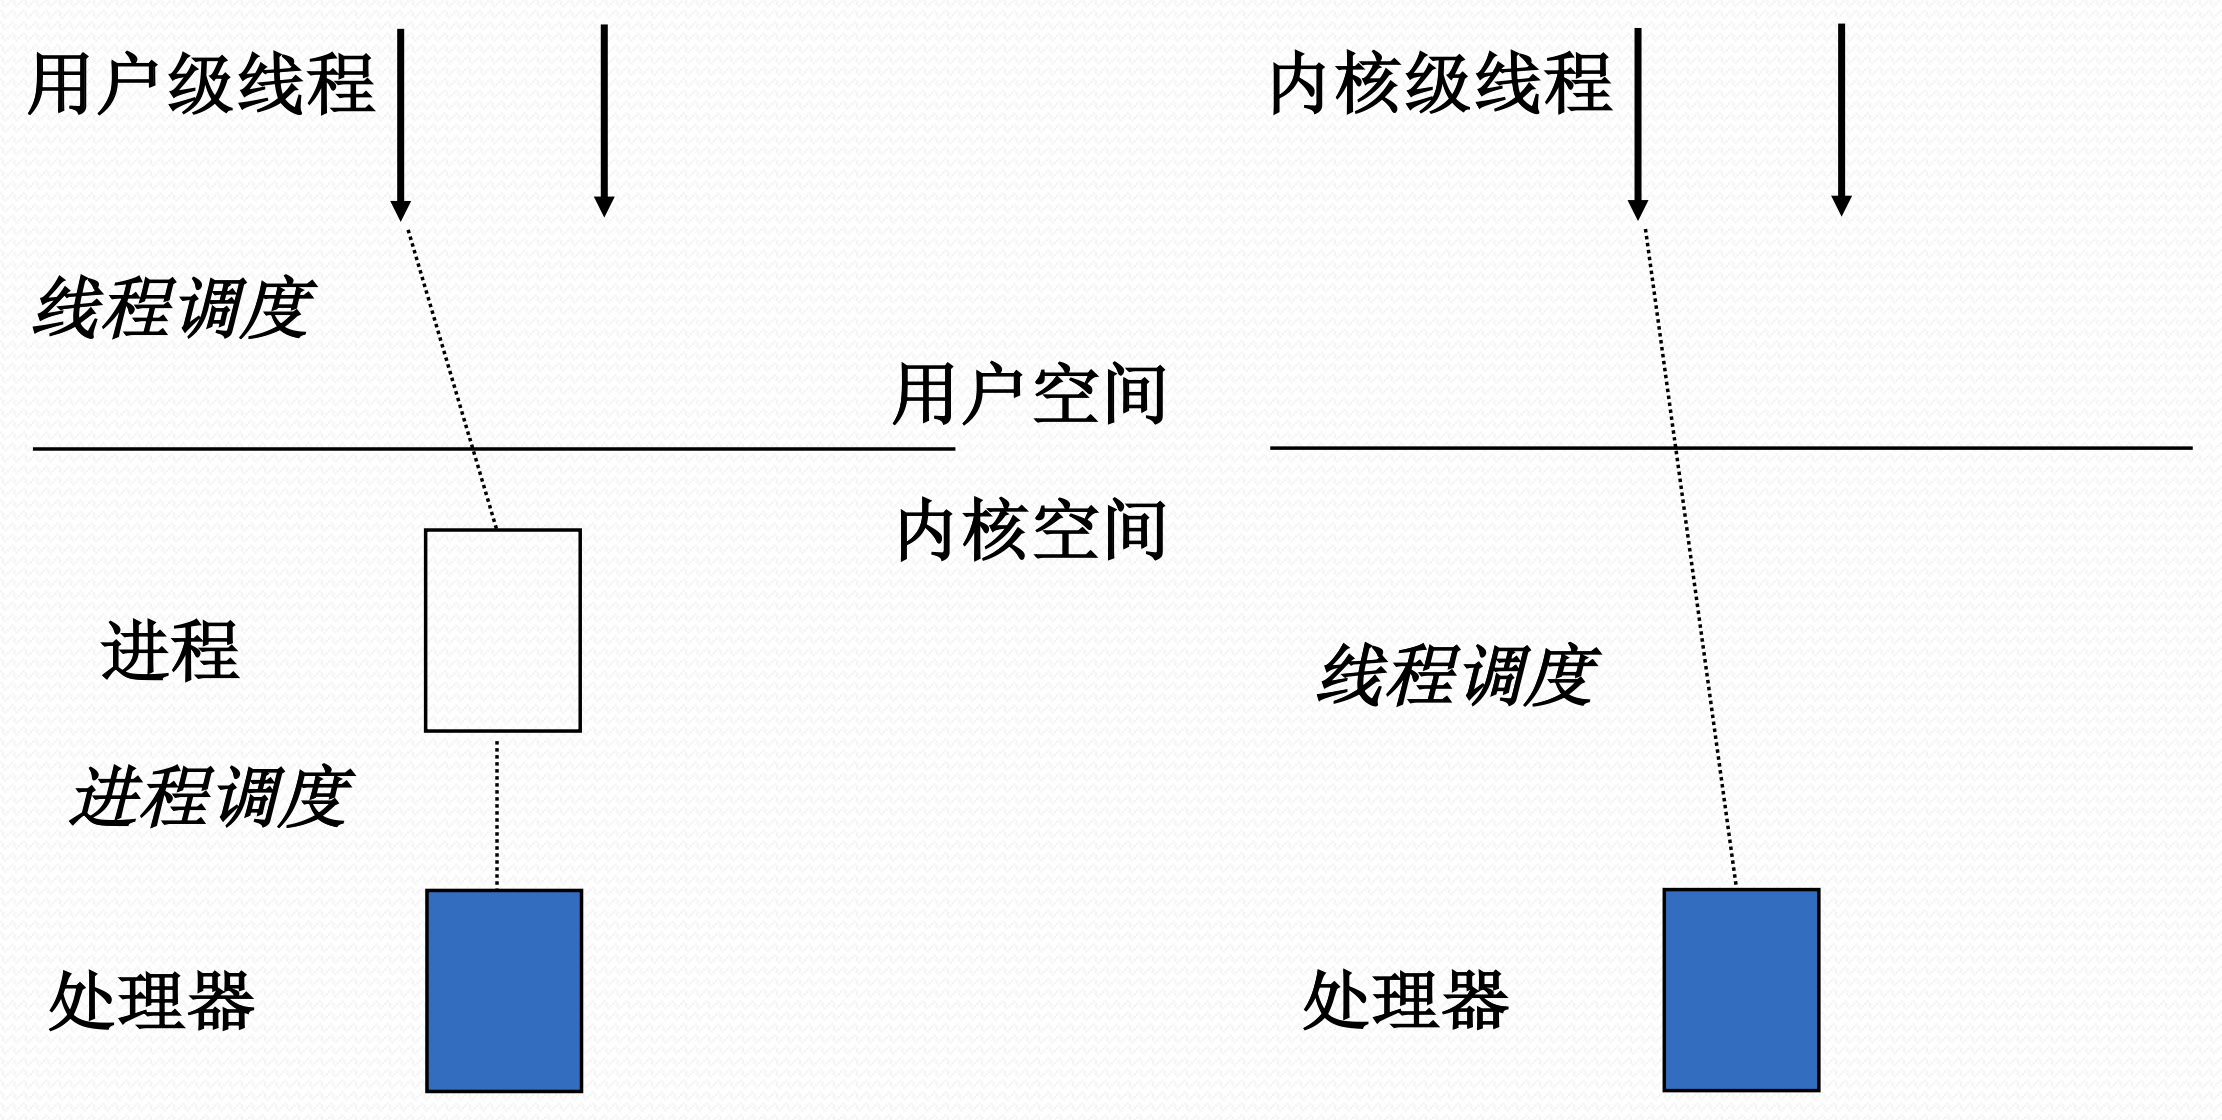
\includegraphics[width=0.5\textwidth]{img/2.4.2.3}
	\end{figure}
	\begin{itemize}
		\item ULT适用于解决逻辑并行性问题
		\item KLT适用于解决物理并行性问题
	\end{itemize}


	\subsection{多线程实现的混合策略}
	\subsubsection{多线程实现的混合策略}
	\begin{itemize}
		\item 在用户空间完成所有的线程的创建工作
		\item 单应用的多个 ULT 可以映射成一些 KLT,通过调整 KLT 数目,可以达到较好的并行效果
		\item 在混合式线程中,内核必须支持内核级多线程的建立、调度和管理,同时也允许应用程序建立、调度和管理用户级线程
		\item 用户级线程的切换仅在用户空间中且仅需要少量机器指令,而内核级线程需要用户态到内核态到用户态的完整上下文切换,修改内存映像,使得高速缓存失效,导致数量级的延迟
	\end{itemize}
	\begin{figure}[H]
		\centering
		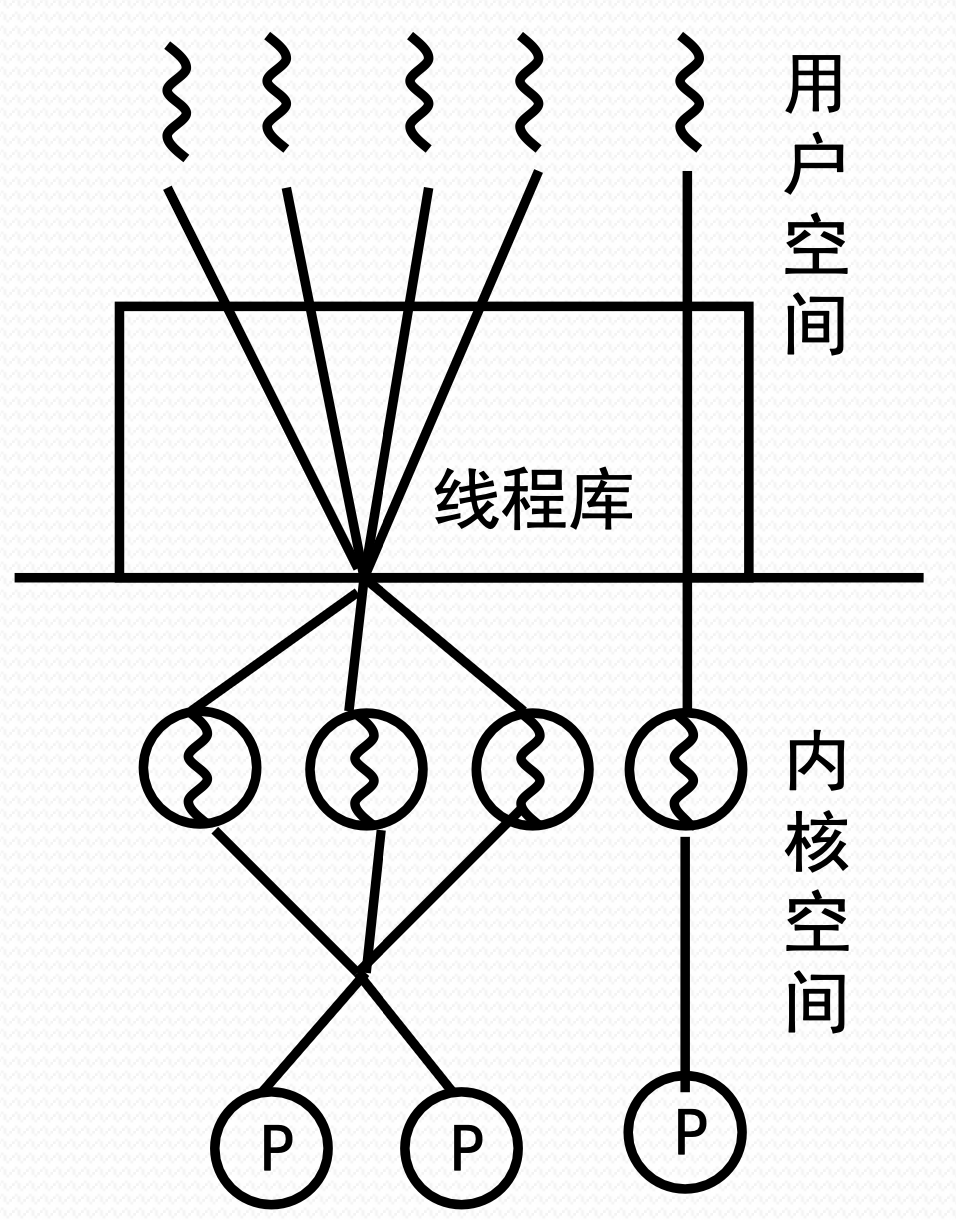
\includegraphics[width=0.35\textwidth]{img/2.4.3.1}
	\end{figure}

	多线程实现混合式策略的特点:
	\begin{itemize}
		\item 合并了用户级线程/内核级线程设施
		\item 线程创建完全在用户空间中完成,线程的调度和同步也在应用程序中进行
		\item 一个应用中的多个用户级线程被映射到一些(小于等于用户级线程数目)内核级线程上
		\item 程序员可以针对特定应用和机器调节内核级线程的数目,以达到整体最佳结果
		\item 该方法将会结合纯粹用户级线程方法和内核级线程方法的优点,同时减少它们的缺点
	\end{itemize}

	\subsubsection{混合式策略下的线程状态}
	\begin{itemize}
		\item KLT 的三态模型,由系统调度负责
		\item ULT 的三态模型,由用户调度负责
		\item 活跃态的 ULT 代表绑定 KLT 的三态
		\item 活跃态的 ULT 运行时可激活用户调度
		\item 非阻塞系统调用可使用 Jacketing 启动用户调度,调整活跃态 ULT
	\end{itemize}
	\begin{figure}[H]
		\centering
		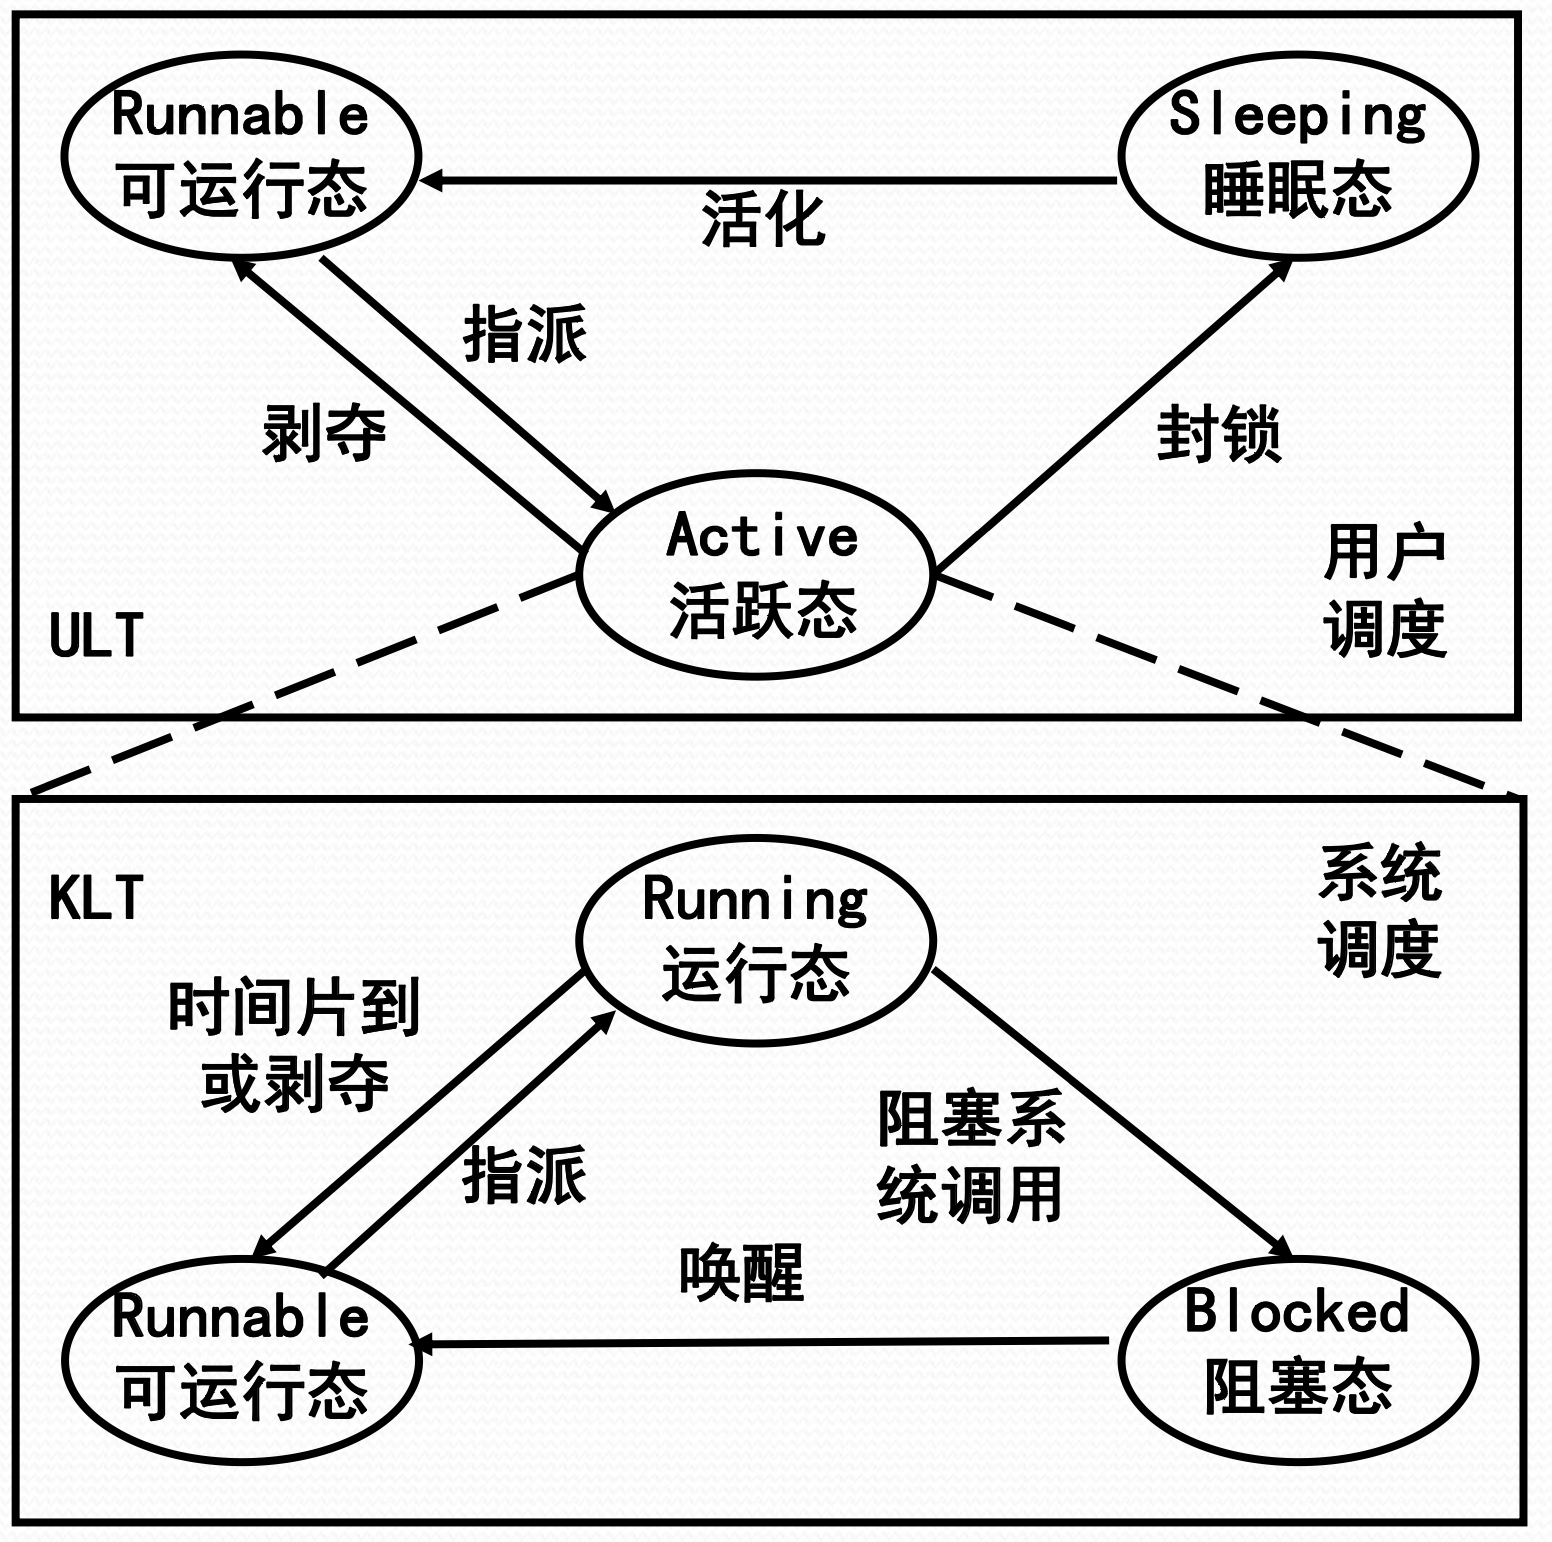
\includegraphics[width=0.45\textwidth]{img/2.4.3.2}
	\end{figure}

	\subsubsection{Solaris多线程技术}
	\begin{figure}[H]
		\centering
		\subfloat[]{
			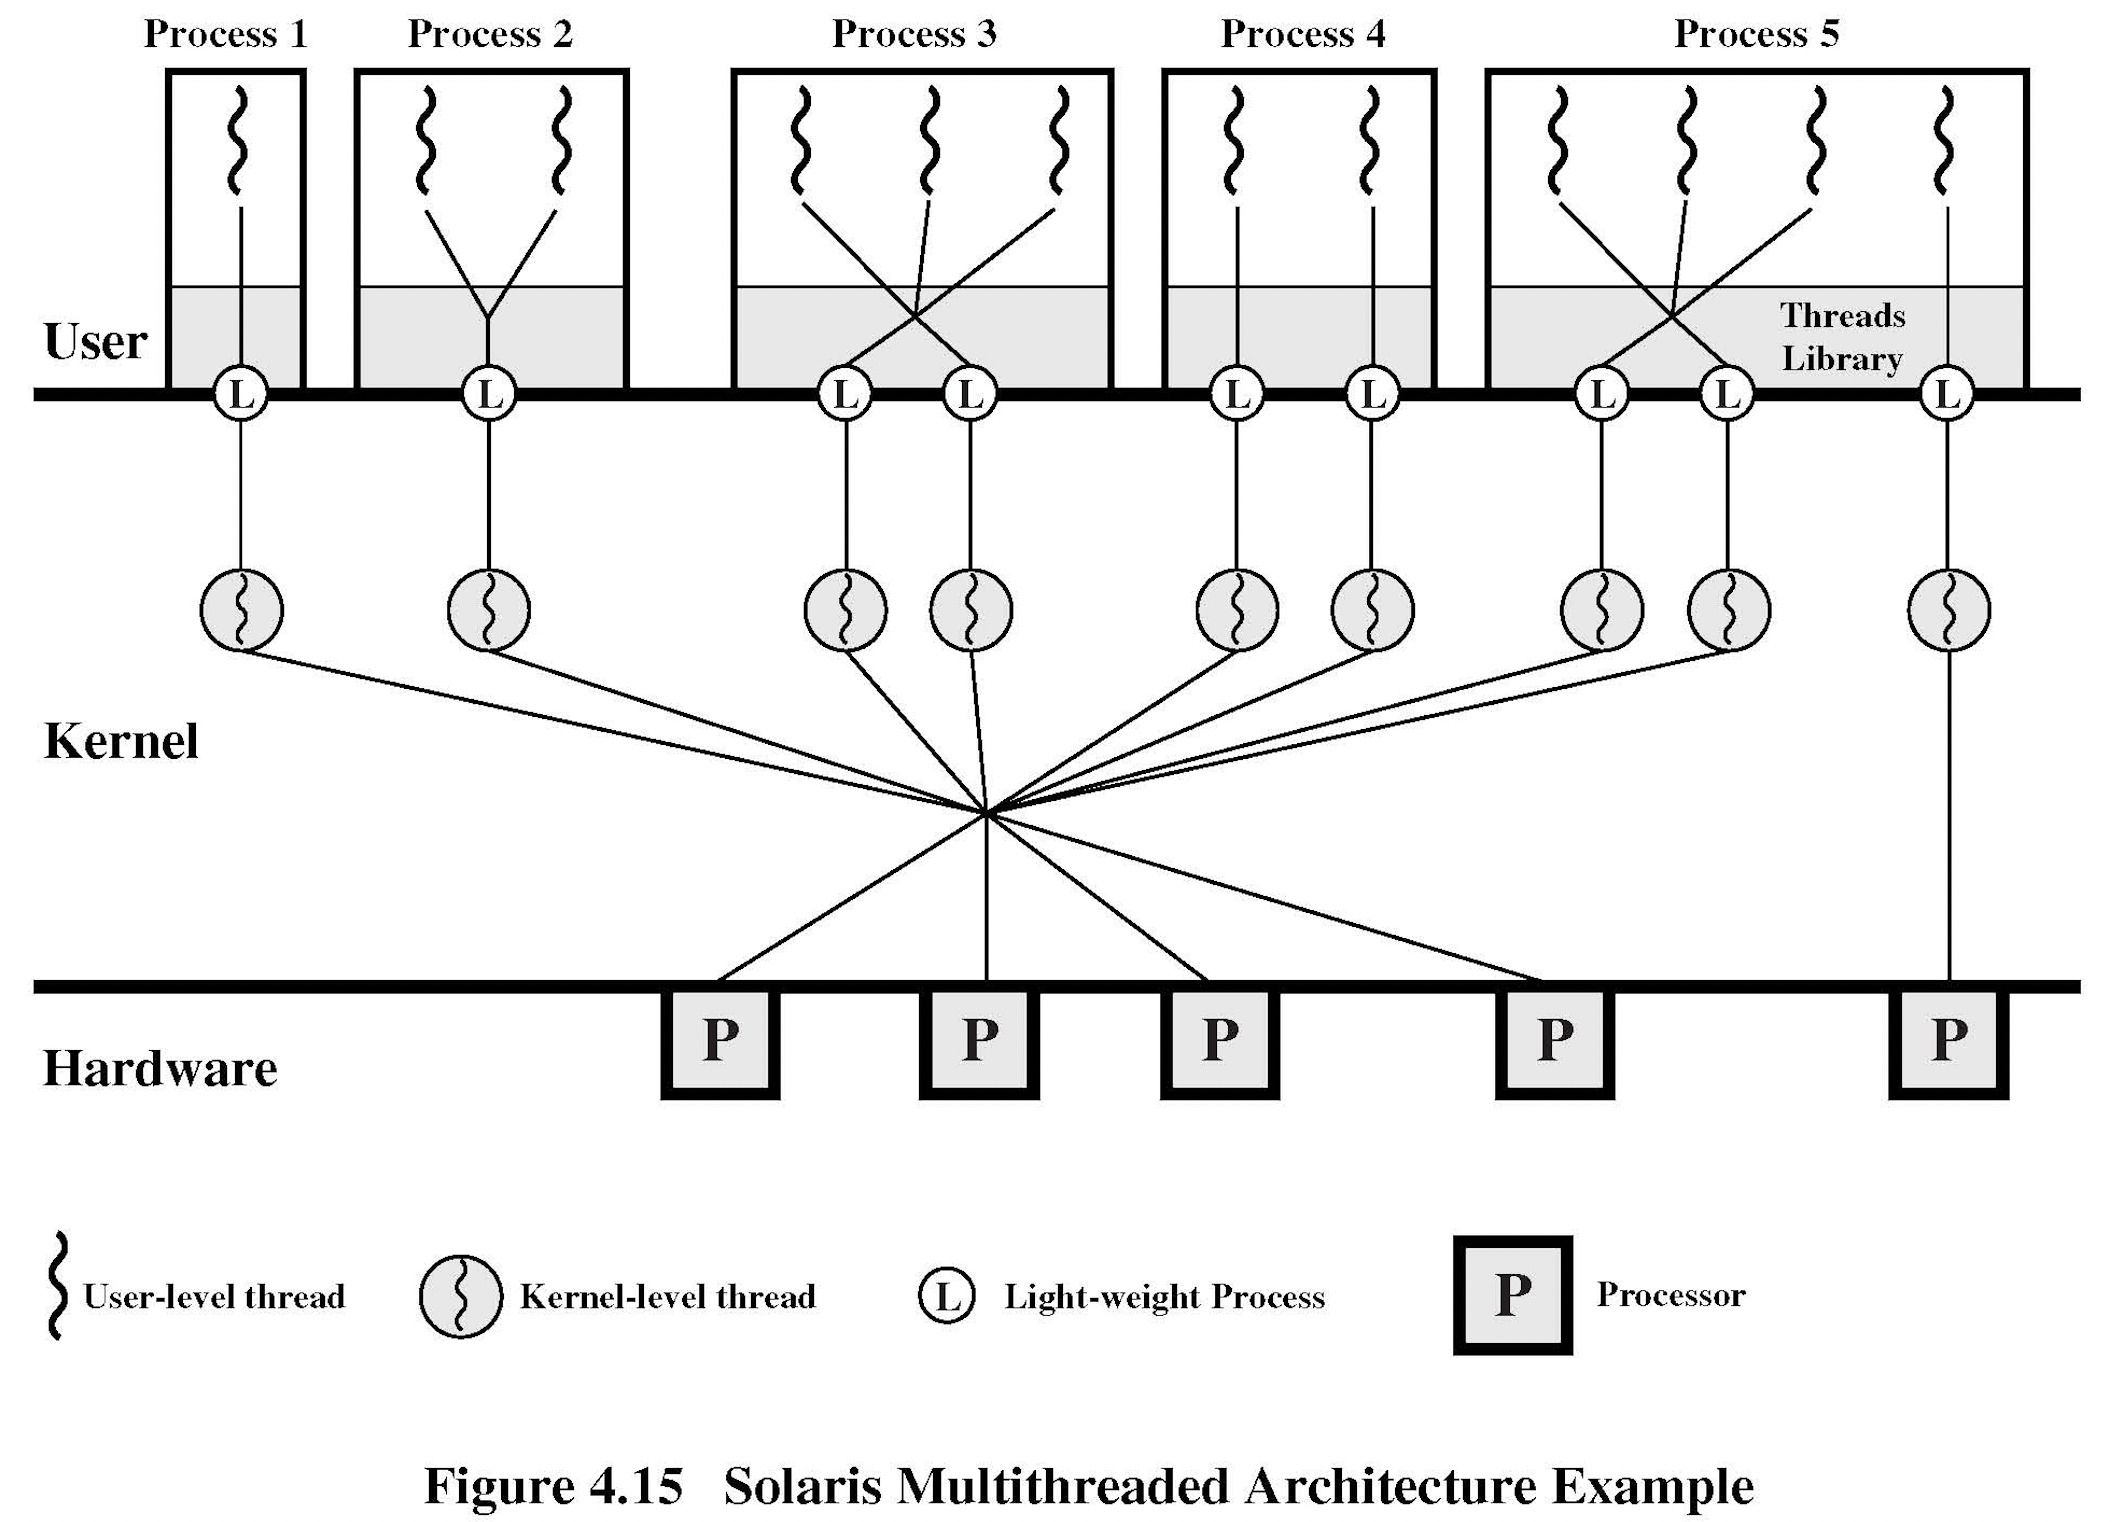
\includegraphics[width=0.6\textwidth]{img/2.4.3.3.1}
		}
		\subfloat[]{
			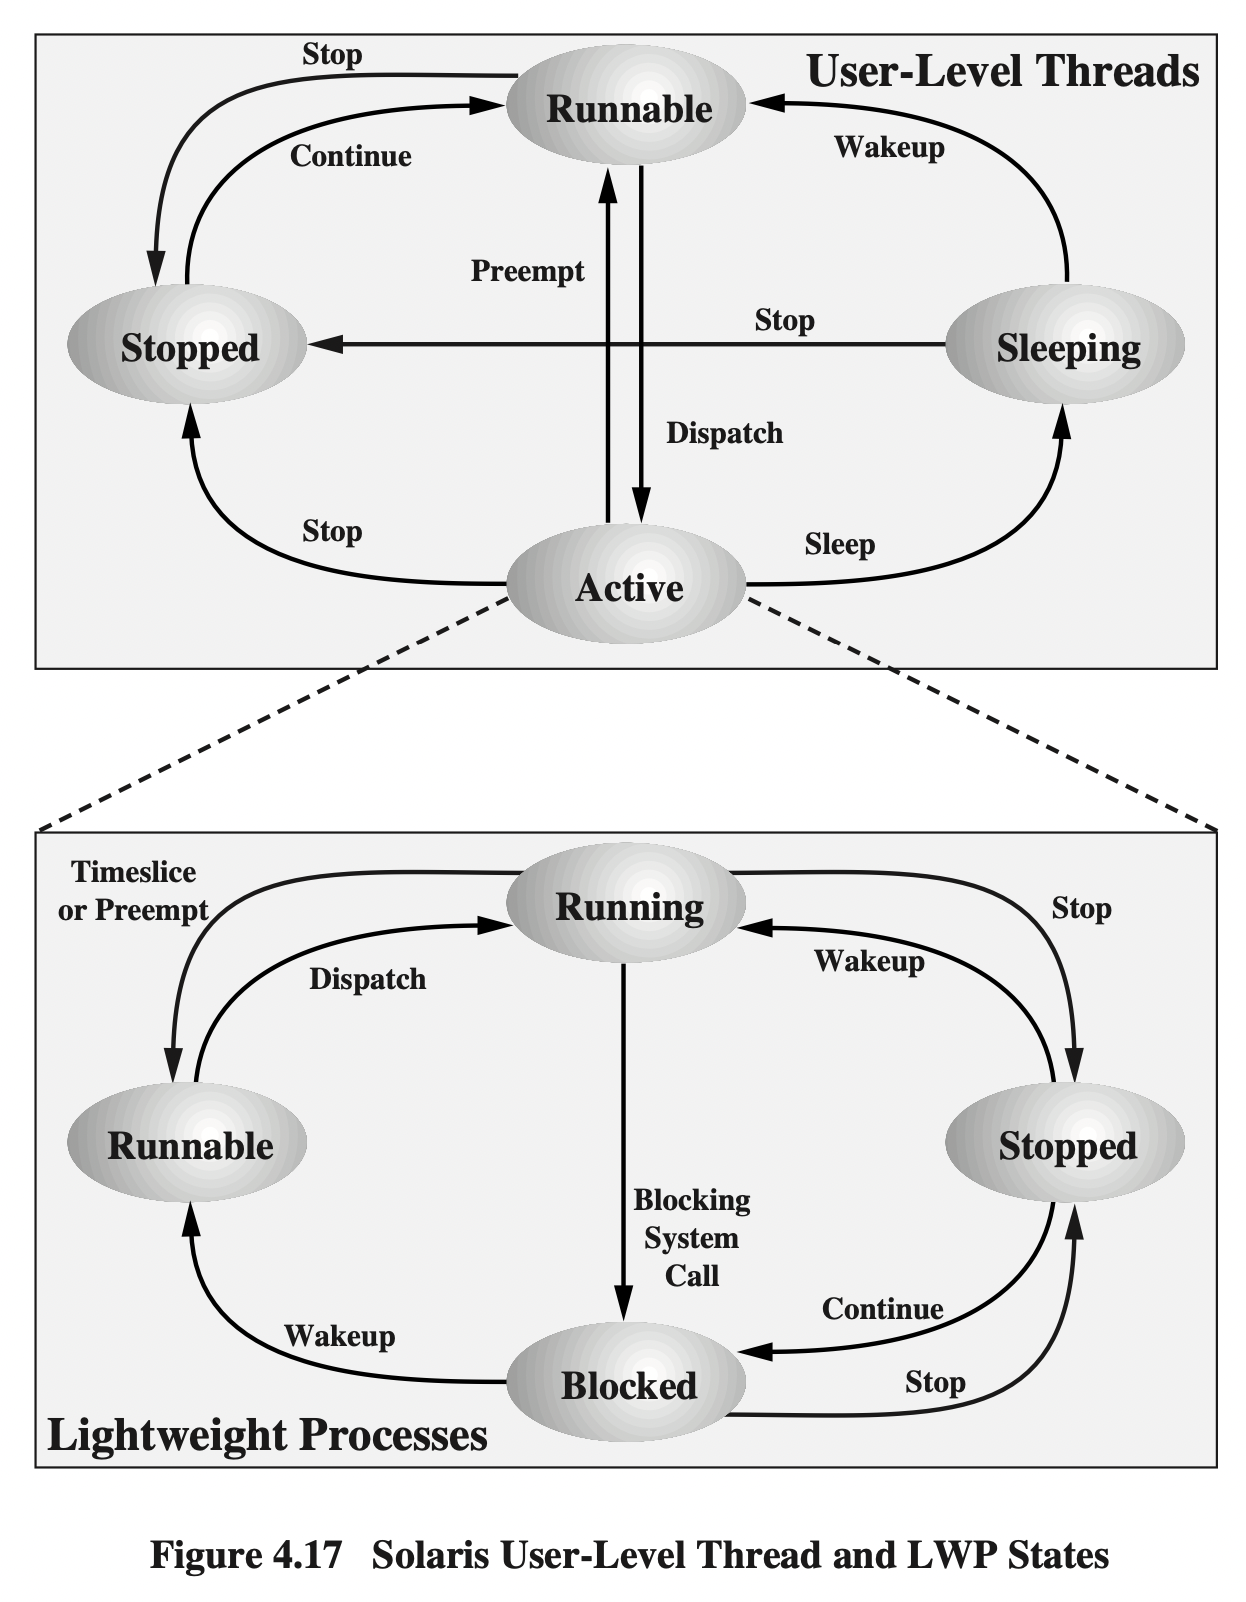
\includegraphics[width=0.35\textwidth]{img/2.4.3.3.2}
		}
	\end{figure}
	包含了多种情况,上图引入了轻量级线程,将轻量级线程与内核级线程映射,原来的多线程设计是Process2,只有一个处理进程,允许给一个进程配置超过一个处理器
	\begin{itemize}
		\item 进程一:单进程单线程,内核级多线程
		\item 进程二:单进程双线程,进程映射到两个轻量级线程,相当于用户级多线程
		\item 进程三:两进程三线程,内核级多线程
		\item 进程四:两进程两线程,内核级多线程
		\item 进程五:三进程四线程,混合级线程,直接做指派意味着线程非常重要,需要单独指派
	\end{itemize}

	一个进程的线程可以被分发到各个位置上并行完成,处理器只能感知进程,不能感知线程,并且只会将一个处理器分配给线程,然后用户空间将得到的处理器分配给线程


	\subsubsection{多线程实现策略的总结}
	\begin{figure}[H]
		\centering
		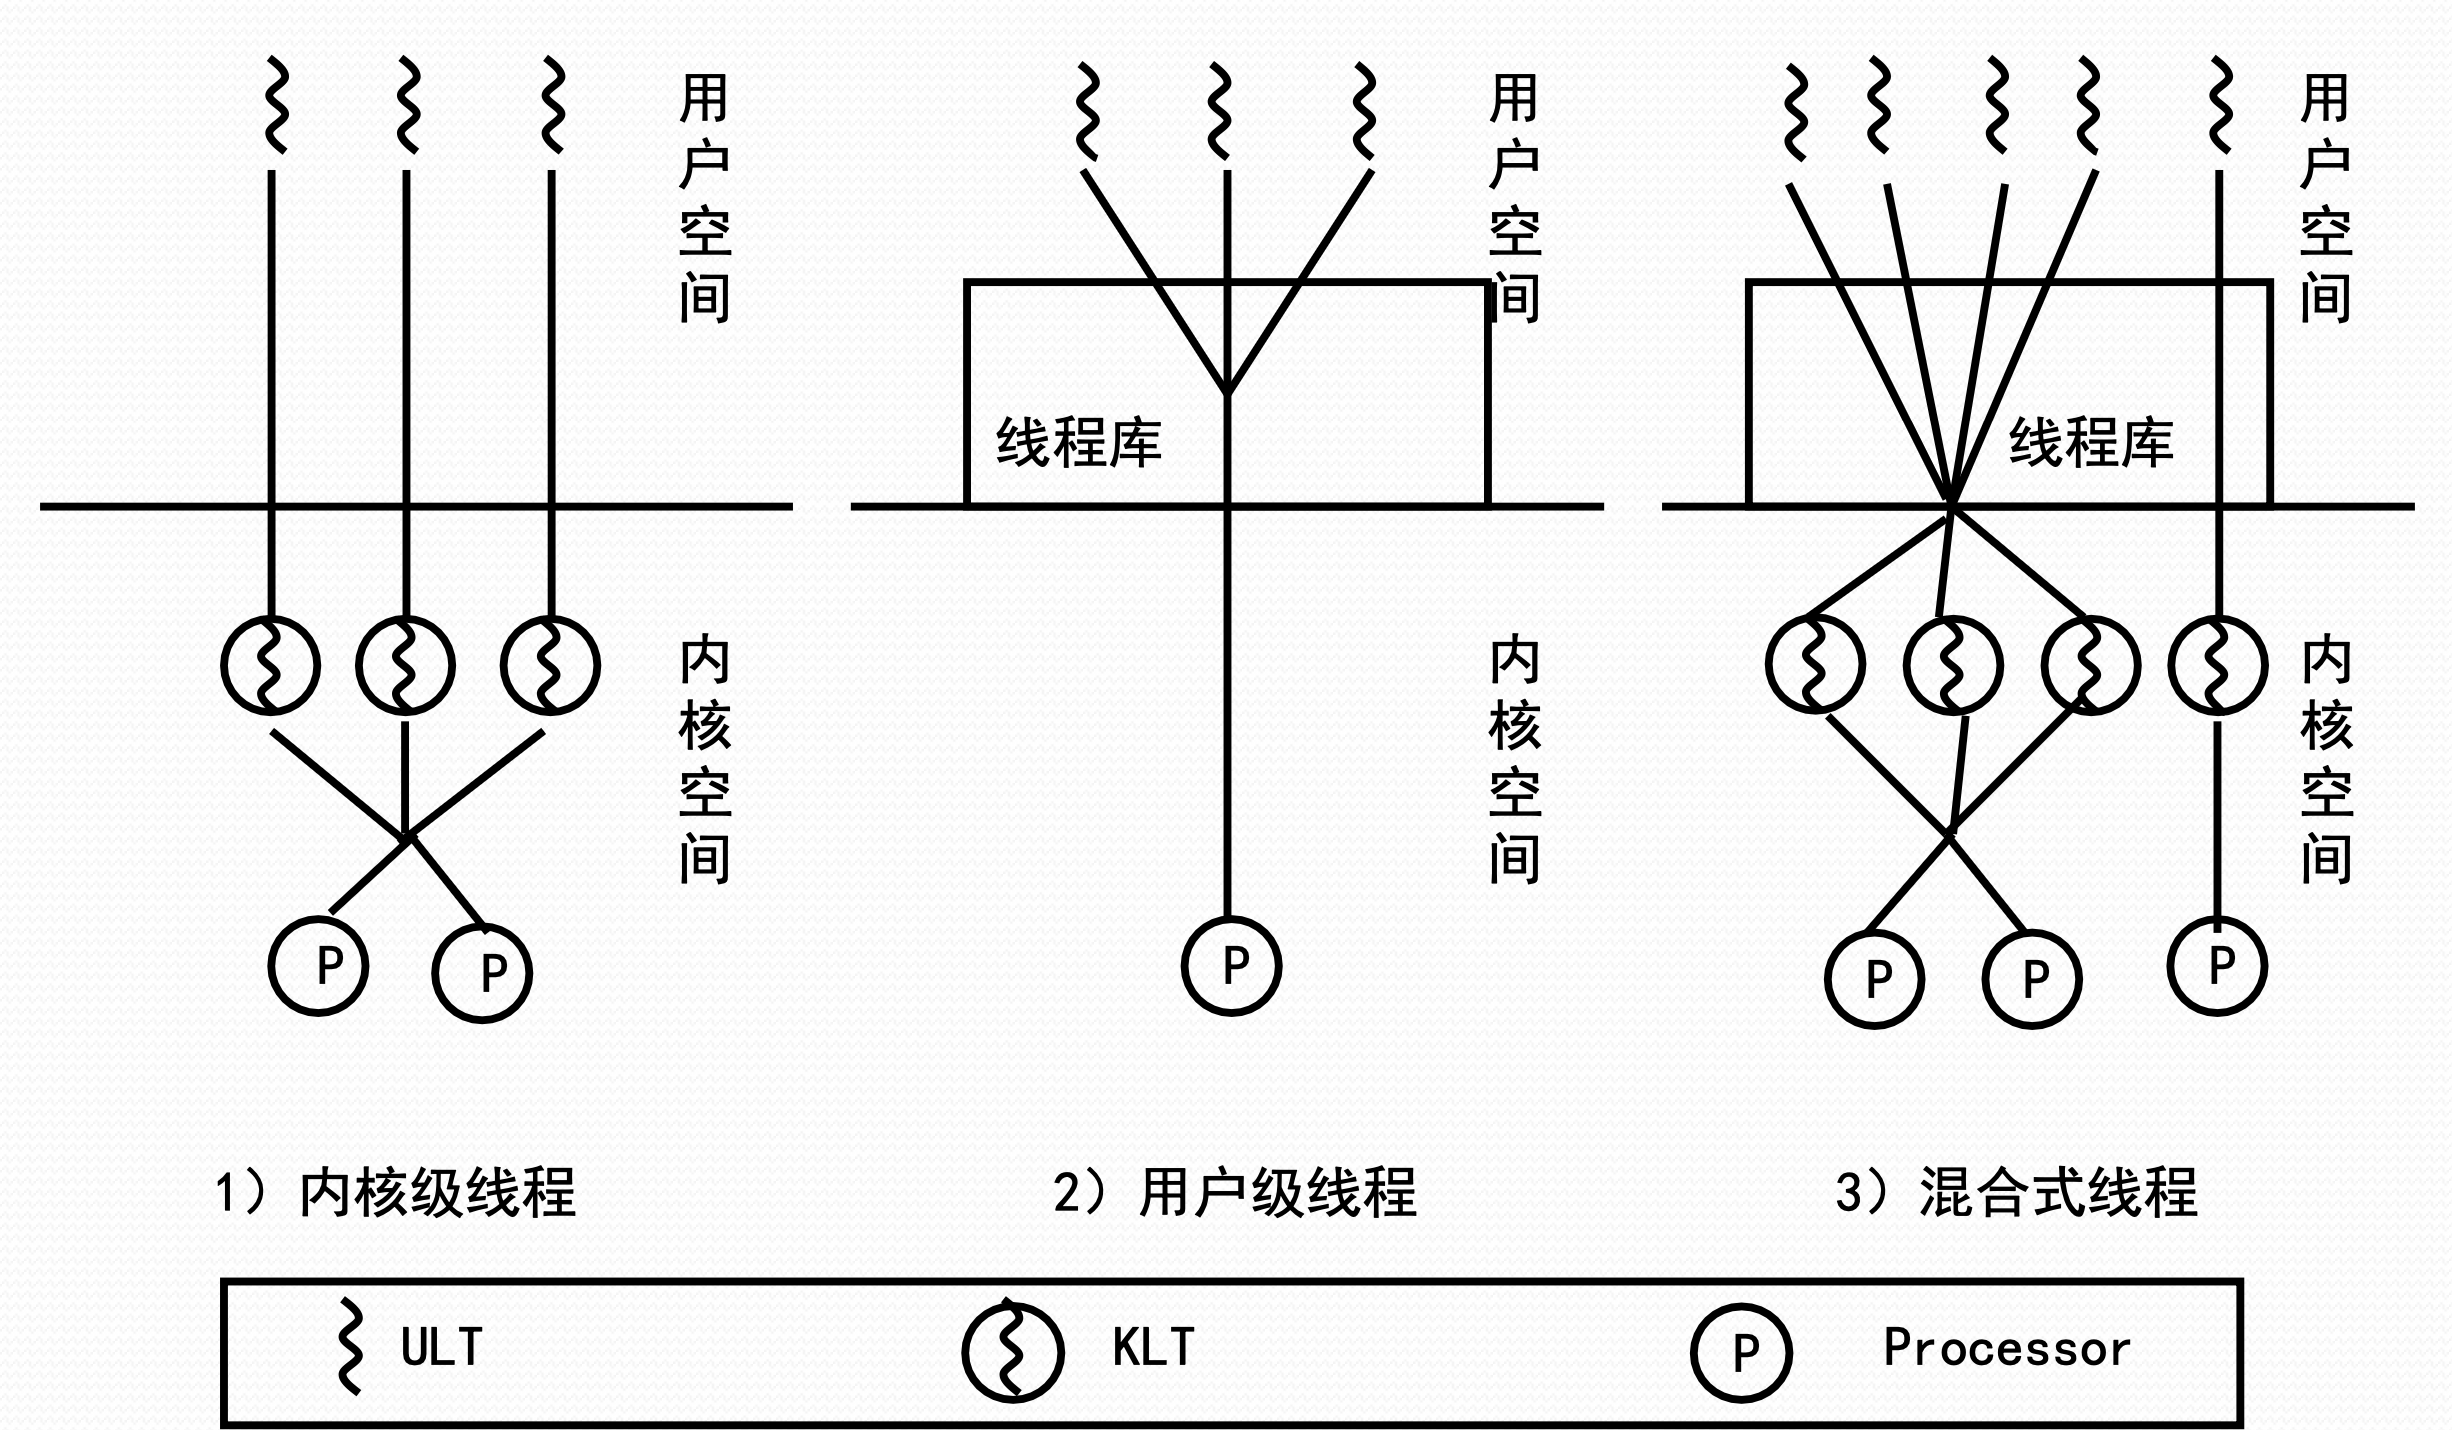
\includegraphics[width=0.7\textwidth]{img/2.4.3.4}
	\end{figure}


	\section{处理器调度}
	\subsection{处理器调度的层次}
	\begin{itemize}
		\item 高级调度:又称长程调度、作业调度,决定能否加入到执行的进程池中,管理从创建进程到调度运行再到结束阶段后的善后部分的全过程
		\item 中级调度,又称平衡调度、中程调度,根据内存资源情况决定内存中所能容纳的进程数目,并完成外存和内存中的进程对换工作
		\item 低级调度:又称短程调度、进程调度/线程调度,根据某种原则决定就绪队列中哪个进程/线程获得处理器,并将处理器让出给它使用
	\end{itemize}

	处理器调度层次与进程状态转换
	\begin{figure}[H]
		\centering
		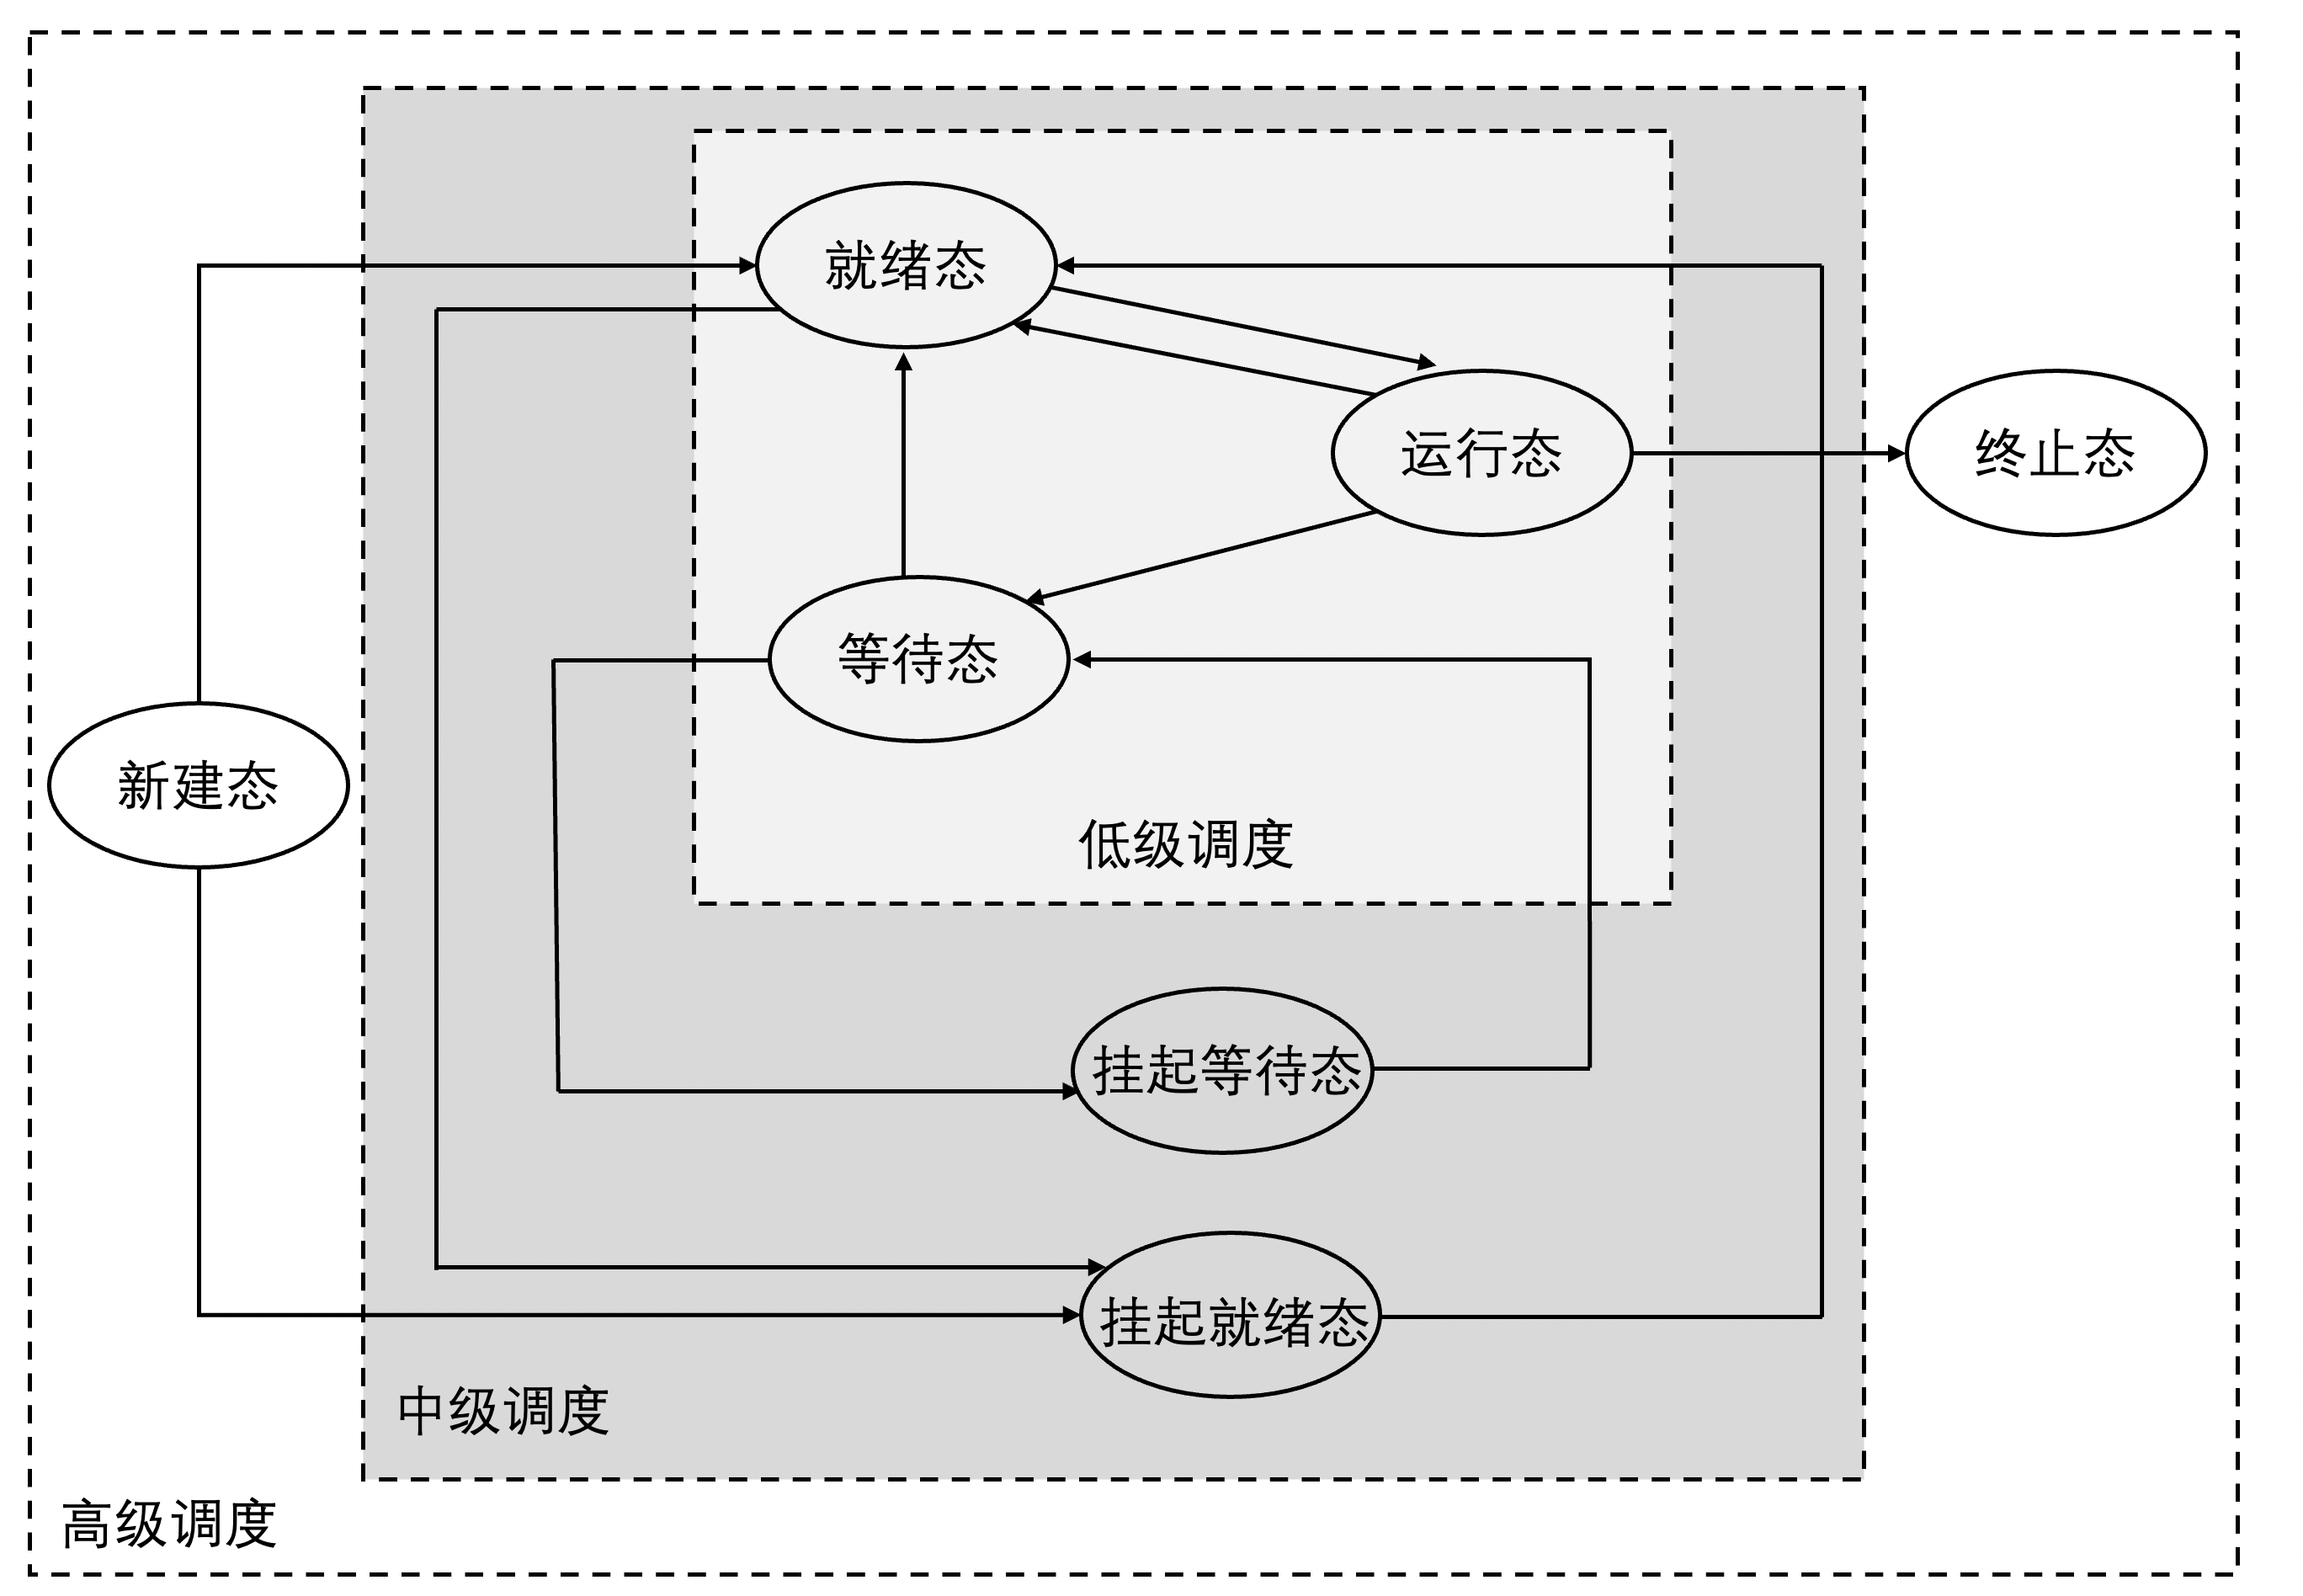
\includegraphics[width=0.6\textwidth]{img/2.5.1}
	\end{figure}

	处理器调度层次与关键状态转换
	\begin{figure}[H]
		\centering
		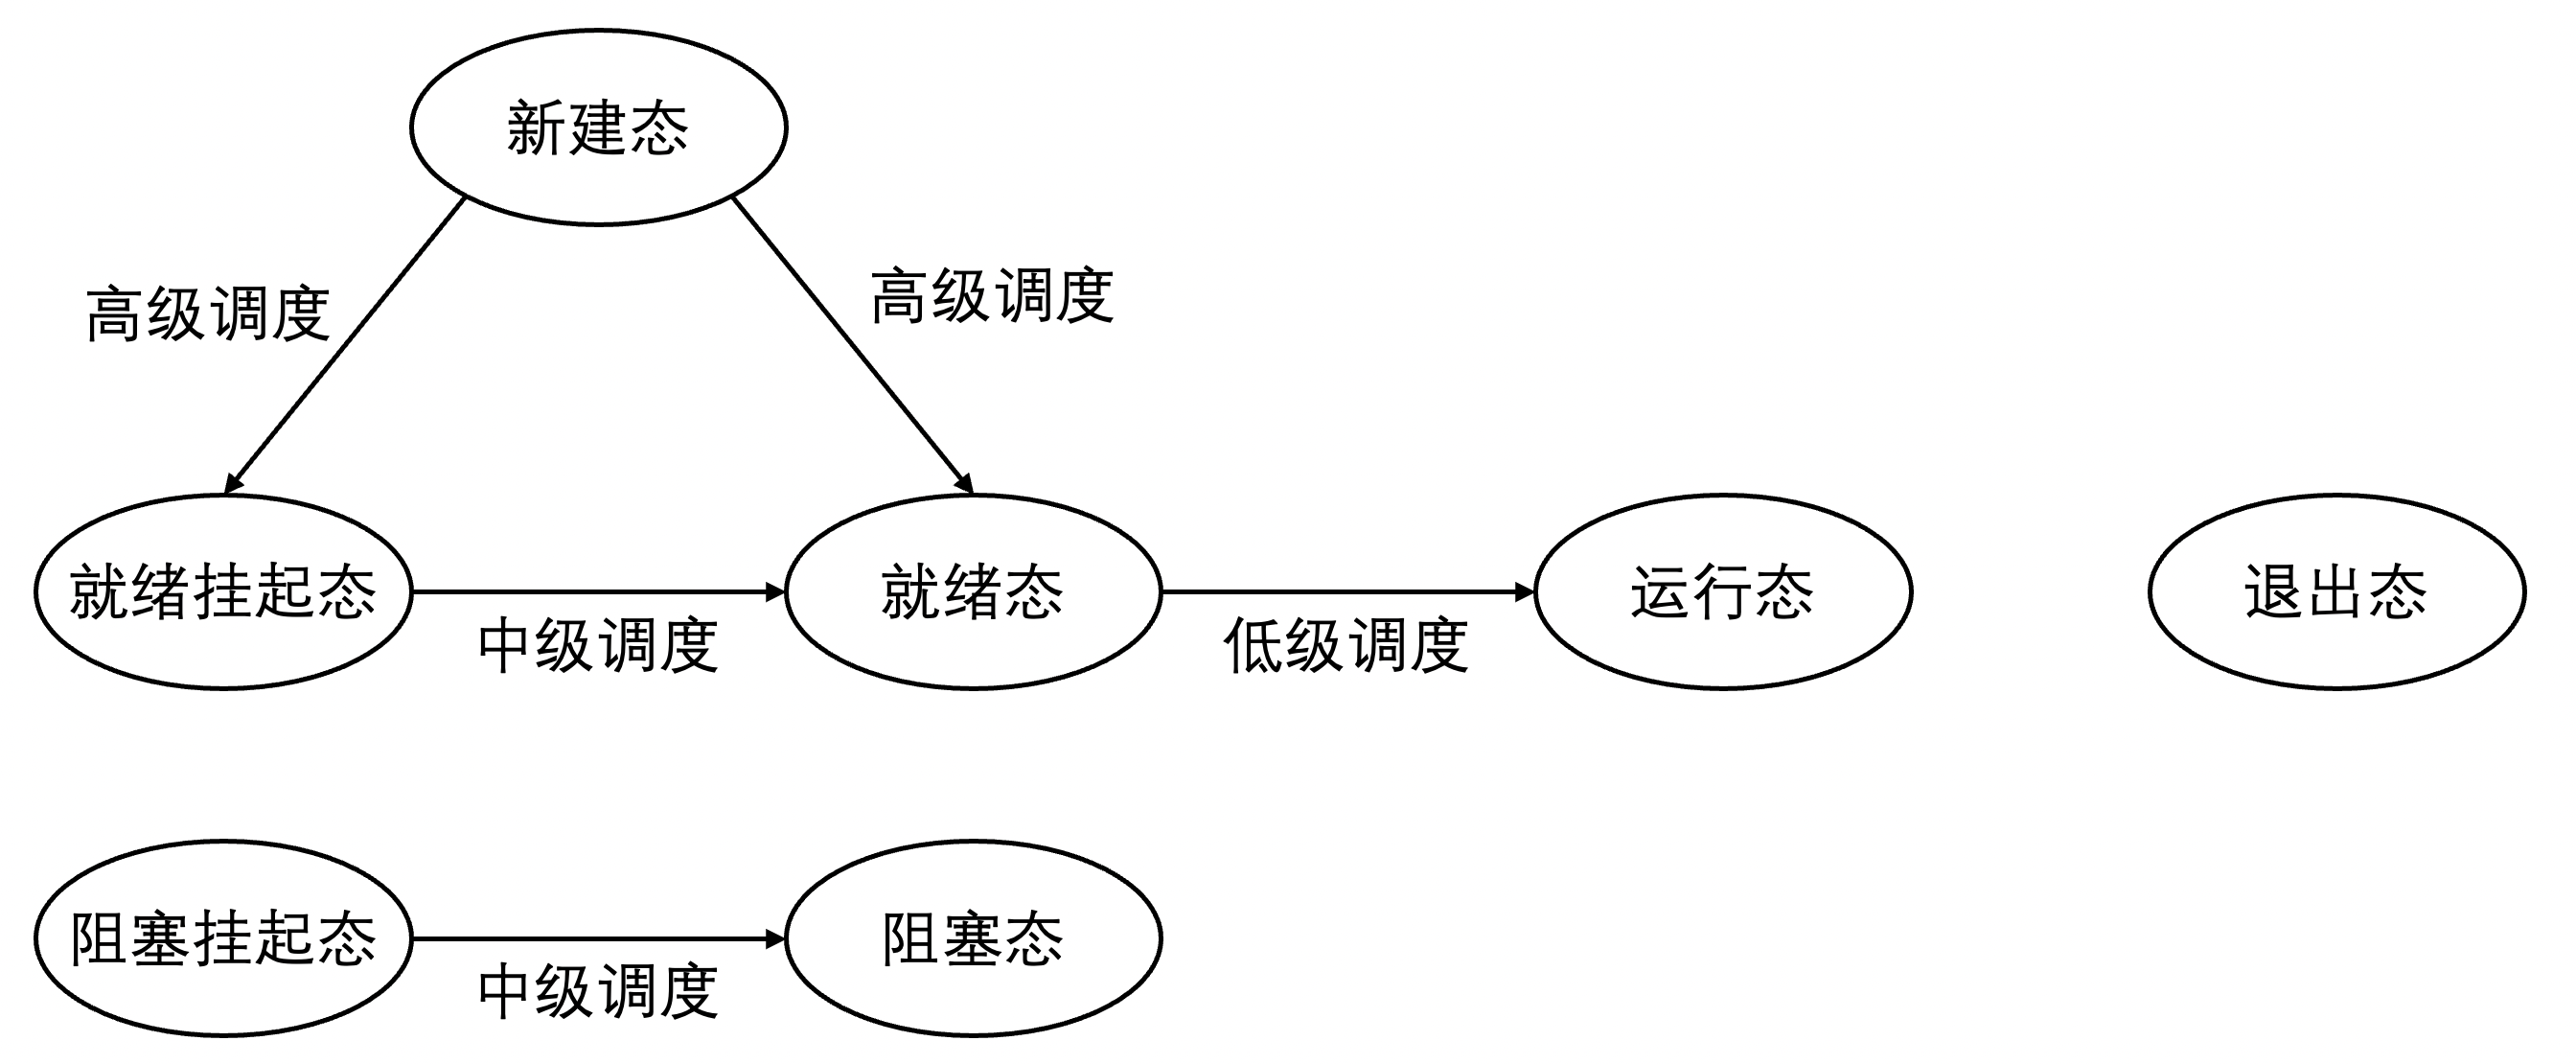
\includegraphics[width=0.6\textwidth]{img/2.5.1.2}
	\end{figure}

	\subsubsection{高级调度}
	分时操作系统中,高级调度决定:
	\begin{itemize}
		\item 是否接受一个终端用户的连接
		\item 命令能否被系统接纳并构成进程
		\item 新建态进程是否加入就绪进程队列
	\end{itemize}

	批处理操作系统中,高级调度又称为作业调度
	\begin{itemize}
		\item 功能是按照某种原则从后备作业队列中选取作业进入主存,并为作业做好运行前的准备工作和完成后的善后工作
	\end{itemize}


	\subsubsection{中级调度}
	\begin{itemize}
		\item 引进中级调度是为了提高内存利用率和作业吞吐量
		\item 中级调度决定那些进程被允许驻留在主存中参与竞争处理器及其他资源,起到短期调整系统负荷的作用
		\item 中级调度把一些进程换出主存,从而使之进入“挂起”状态,不参与进程调度,以均衡系统的负载
	\end{itemize}


	\subsubsection{低级调度}
	\begin{itemize}
		\item 低级调度又称处理器调度、进程调度、短程调度,按照某种原则把处理器分配给就绪态进程或内核级线程
		\item 进程调度程序,又称分派程序,操作系统中实现处理器调度的程序,是操作系统的最核心部分
		\item 处理器调度策略的优劣直接影响到整个系统的性能
		\item 低级调度的主要功能:
		\begin{itemize}
			\item 记住进程或内核级线程的状态
			\item 决定某个进程或内核级线程什么时候获得处理器,以及占用多长时间
			\item 把处理器分配给进程或内核级线程
			\item 收回处理器
		\end{itemize}
	\end{itemize}
	处理器三级调度的队列模型
	\begin{figure}[H]
		\centering
		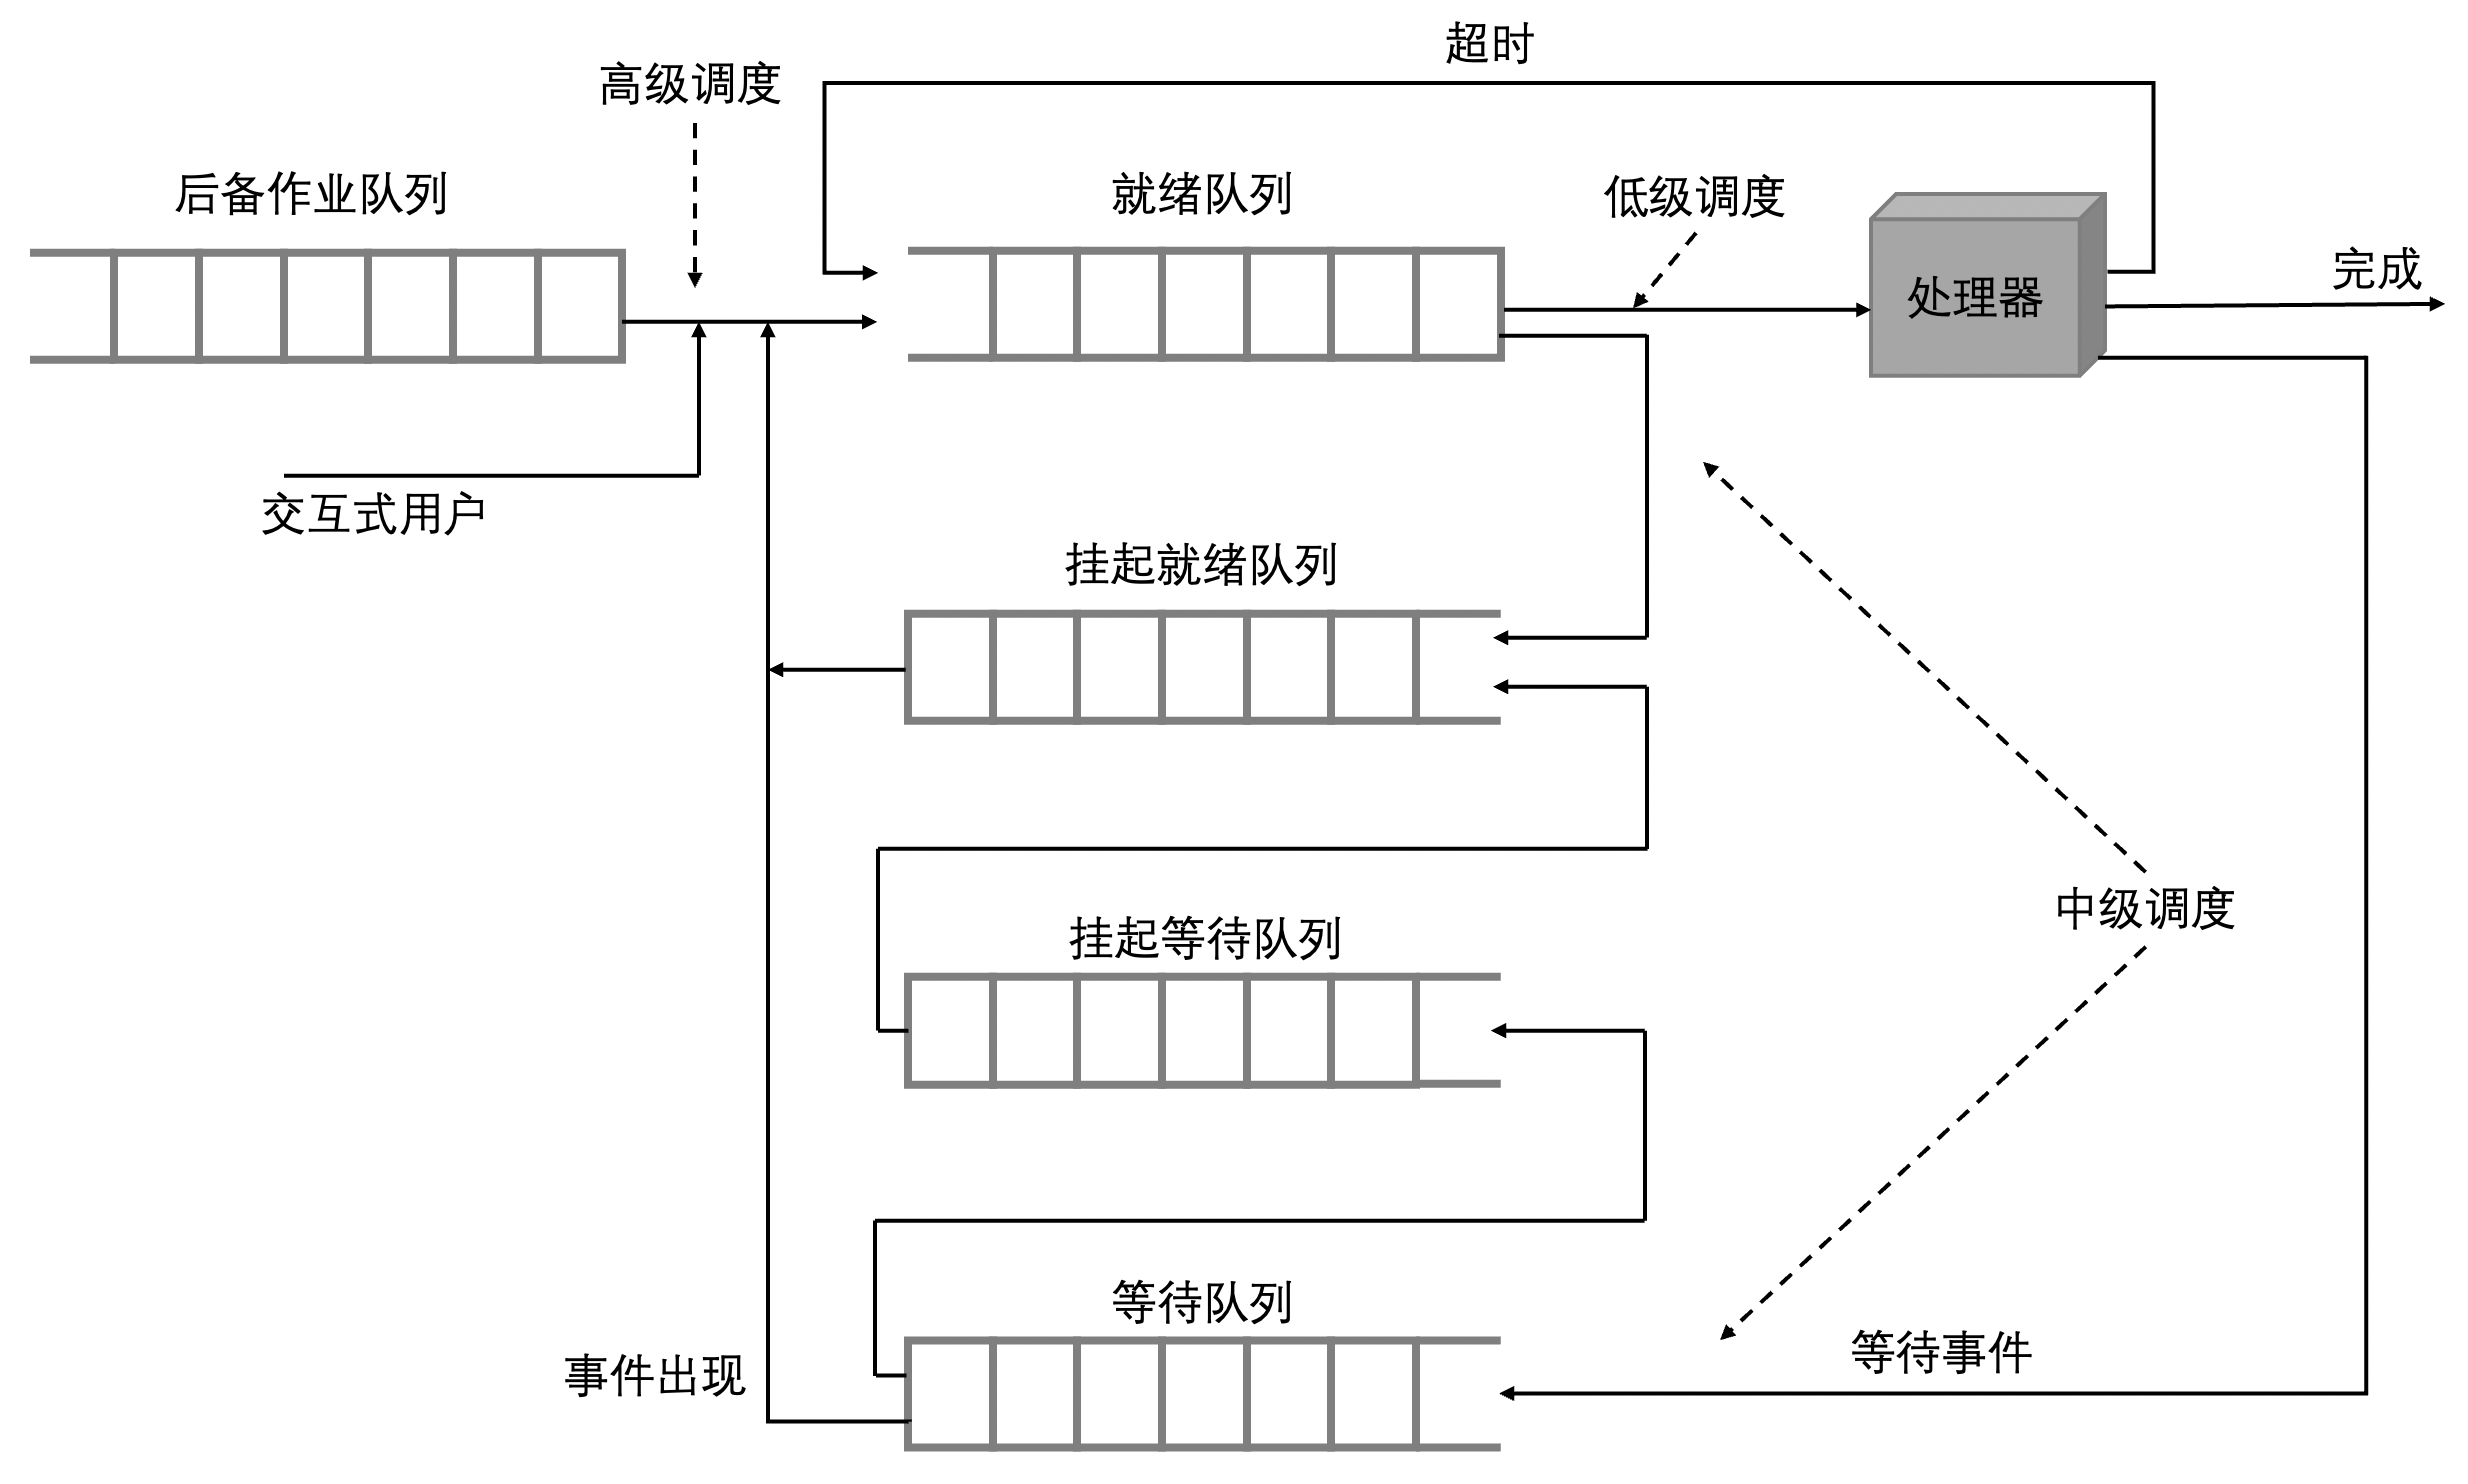
\includegraphics[width=0.75\textwidth]{img/2.5.1.3}
	\end{figure}

	\subsection{处理器调度算法}
	\subsubsection{选择处理器调度算法的原则}
	\begin{itemize}
		\item 资源利用率:使得 CPU 或其他资源的使用率尽可能高且能够并行工作
	\end{itemize}

	\begin{align*}
		\mathrm{CPU}\mbox{利用率} & =\frac{\mathrm{CPU}\mbox{有效工作时间}}{\mathrm{CPU}\mbox{总运行时间}}  \\
		\mathrm{CPU}\mbox{总运行时间} & = \mathrm{CPU}\mbox{有效工作时间} + \mathrm{CPU}\mbox{空闲等待时间}
	\end{align*}

	\begin{itemize}
		\item 吞吐量:单位时间处理的进程数尽可能多
		\item 公平性:确保每个用户每个进程获得合理的 CPU 份额或其他资源份额
		\item 响应时间:
		\begin{itemize}
			\item 使交互式用户的响应时间尽可能小,或尽快处理实时任务
			\item 细分包含输入的程序命令传送到 CPU 时间、CPU 处理请求命令的时间、处理所形成的响应回送到终端显示器的时间
		\end{itemize}
		\item 周转时间:提交给系统开始到执行完成获得结果为止的这段时间间隔称周转时间,应该使周转时间或平均周转时间尽可能短
	\end{itemize}
	\begin{align*}
		\mbox{作业}i\mbox{周转时间}t_i & = \mbox{完成时刻}t_f - \mbox{提交时刻} t_s \\
		\mbox{平均作业周转时间}T & = \frac{\sum \limits_{i=1}\limits^nt_i}{n}\\
		\mbox{作业带权周转时间}w_i & = \frac{\mbox{周转时间}t_i}{\mbox{运行时间}t_k} \\
		\mbox{平均带权做作业周转时间}W & =  \frac{\sum\limits_{i=1}\limits^nw_i}{n}
	\end{align*}

	\subsubsection{优先数调度算法}
	优先数调度就是给每个进程或作业规定一个优先数,先满足优先数高的,再满足优先数低的
	\begin{itemize}
		\item 既适用于作业调度,也适用于进程或内核线程调度
	\end{itemize}

	对于进程或内核线程调度,优先数调度算法有两种策略:
	\begin{itemize}
		\item 抢占式优先数调度
		\begin{itemize}
			\item 有更高优先级进程出现时立即占有 CPU 运行
			\item 对于硬实时操作系统是必须的
		\end{itemize}
		\item 非抢占式优先数调度
		\begin{itemize}
			\item 等待 CPU 空闲之后才启动调度程序去选择高优先级进程占有 CPU 运行
			\item 适合大多数操作系统
		\end{itemize}
	\end{itemize}

	决定优先数的方式有很多种:
	\begin{itemize}
		\item 作业或进程负担任务的紧迫程度
		\item 进程的交互性
		\item 进程使用外设的额度
		\item 进程进入系统的时间长短
		\item 公平性等
	\end{itemize}

	目前已有的与进入系统时间或系统处理时间香港的优先数调度算法
	\begin{itemize}
		\item 先来先服务(first come first served,FCFS)调度算法
		\item 最短进程优先(shortest process first,SPF)调度算法
		\item 最短剩余时间优先(shortest remaining time first,SRTF)调度算法
		\item 最高响应比优先(highest response ratio first,HRRF)调度算法
	\end{itemize}

	\paragraph{先来先服务FCFS}~{}

	先来先服务算法是\textbf{非抢占式}调度,按照进程进入系统的时间顺序排序

	常用于批处理系统的高级调度和分时系统的中断连接

	一般不适用于进程调度
	\begin{itemize}
		\item 以计算为主的进程在此策略下过于优越
		\item 容易造成这些进程长时间占用处理器,大幅延长了其他进程的周转时间,降低了系统进程的吞吐率
	\end{itemize}

	\begin{figure}[H]
		\centering
		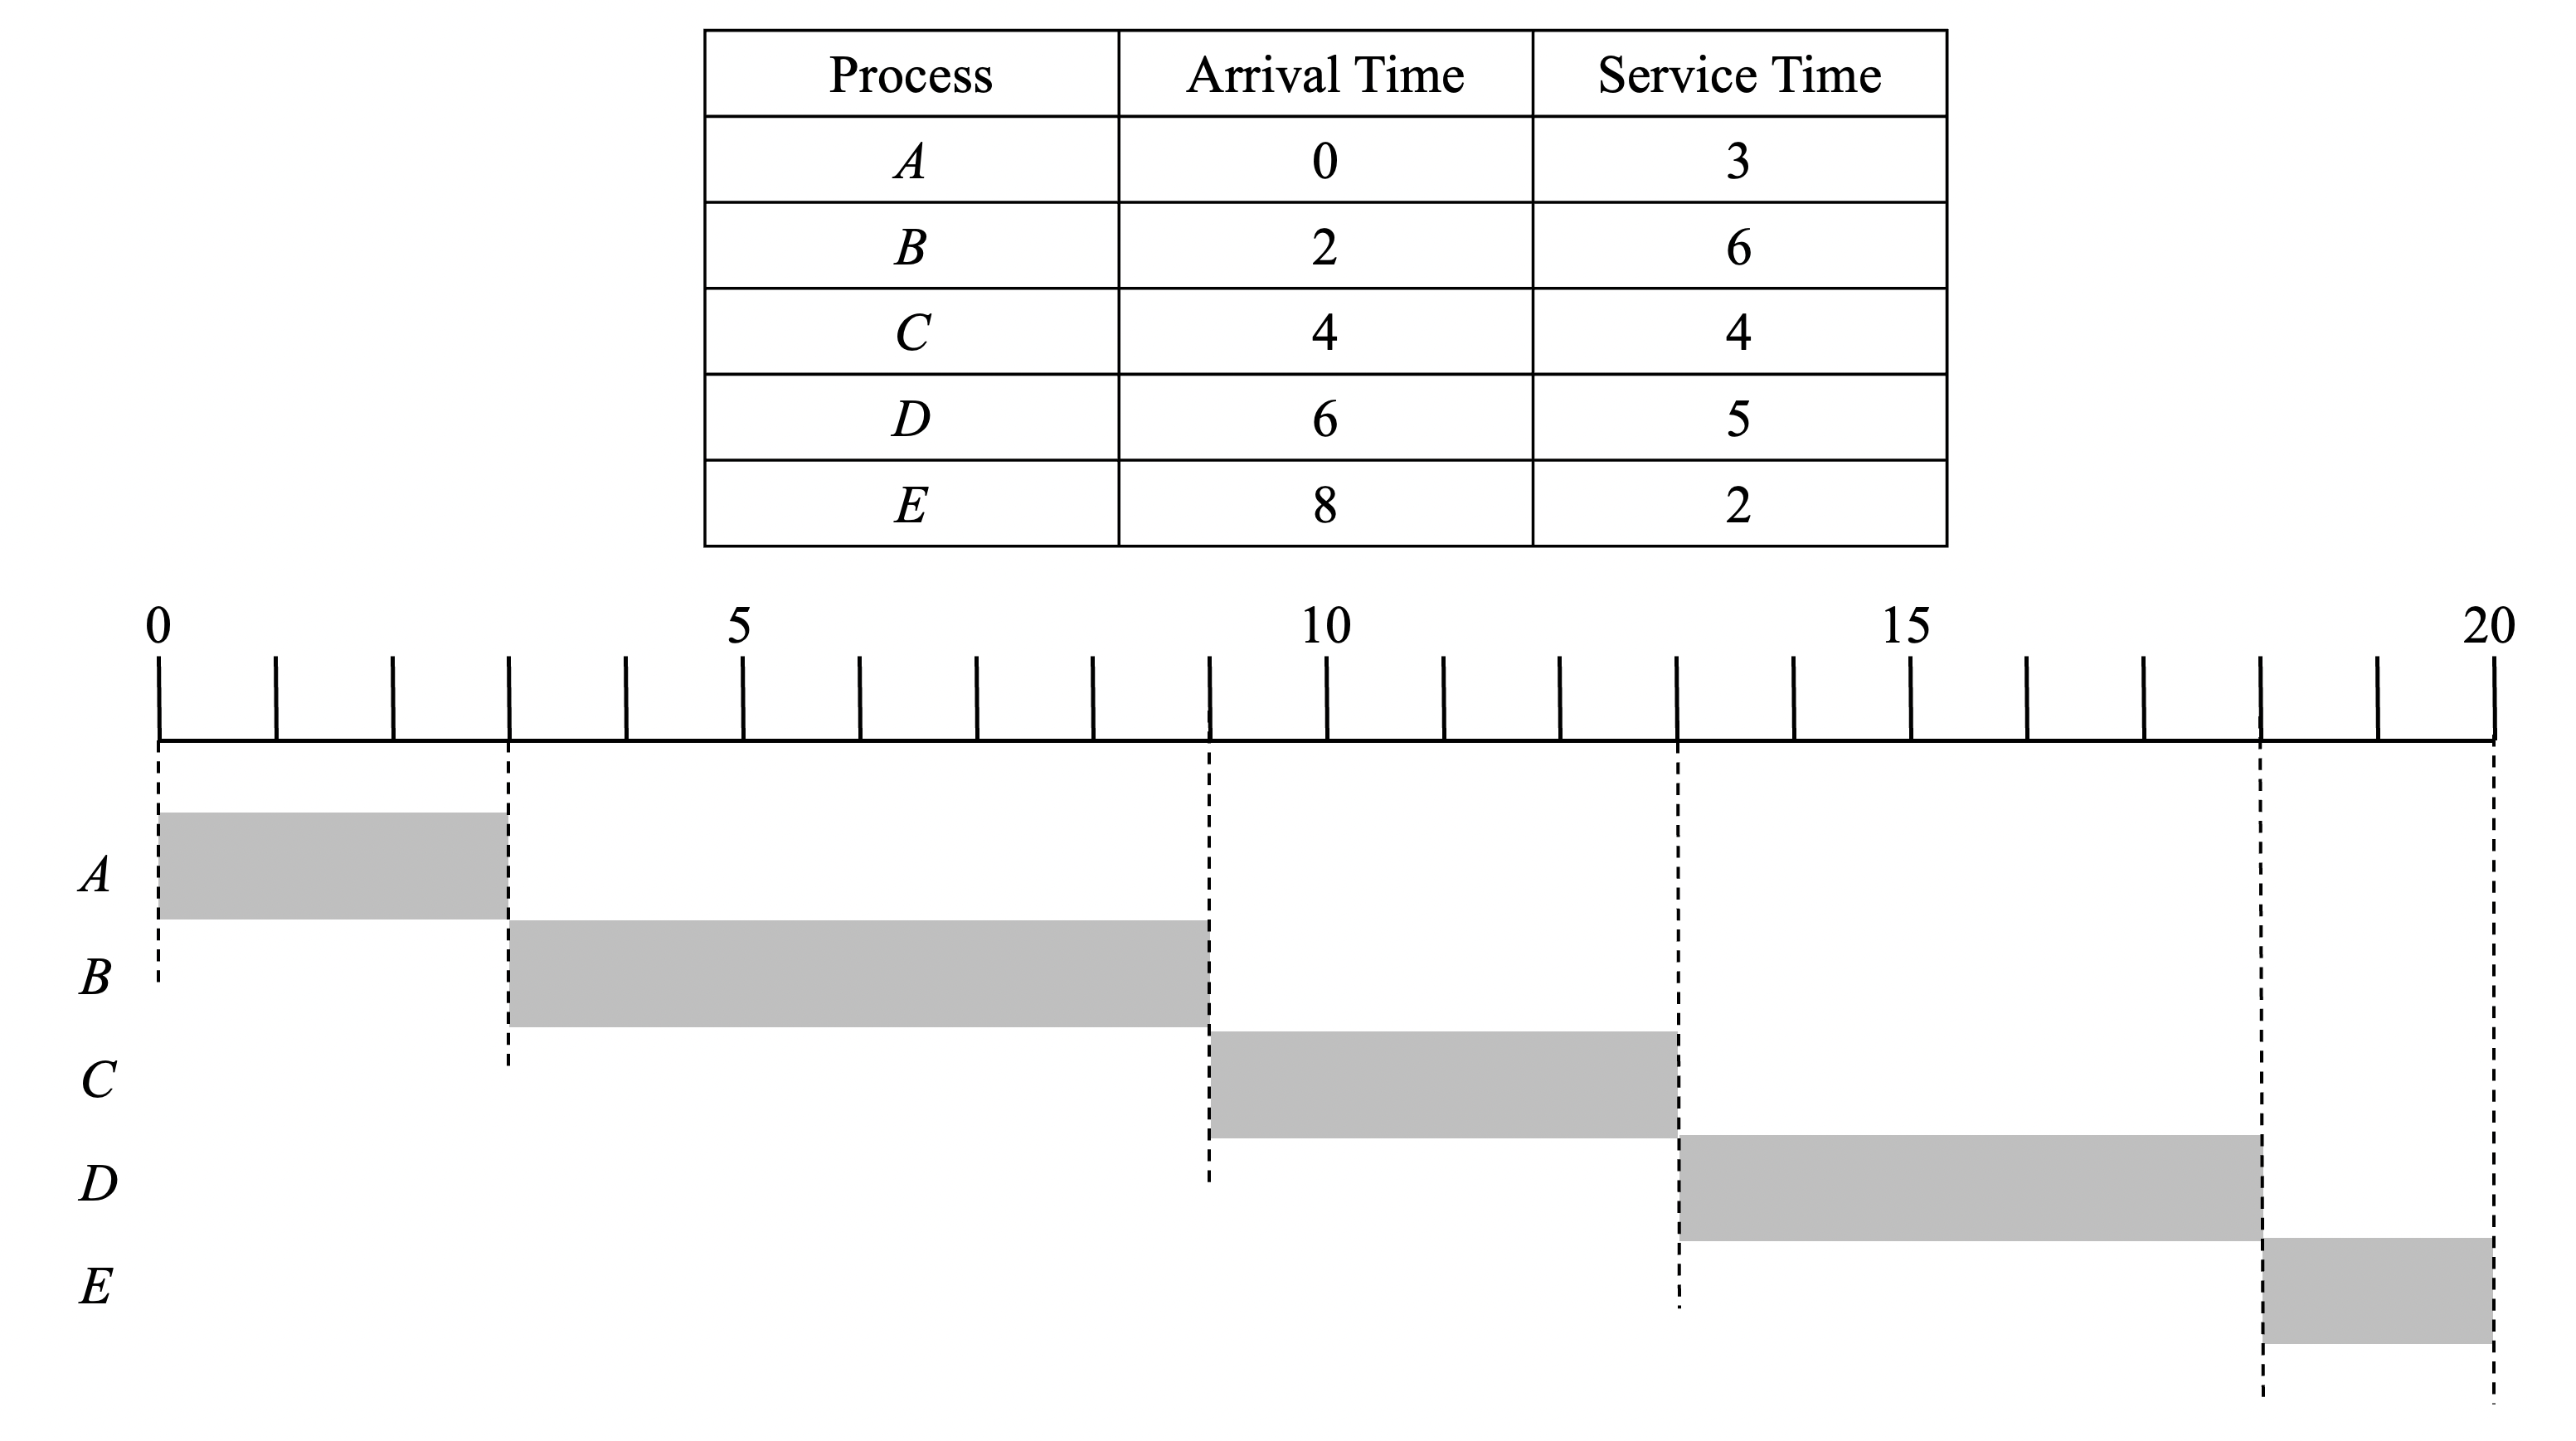
\includegraphics[width=0.65\textwidth]{img/FCFS}
	\end{figure}

	\paragraph{最短进程优先SPF}~{}

	最短进程优先是\textbf{非抢占式}调度,优先处理计算时间短的进程,有利于提高系统的吞吐率和平均周转率,但该原则对计算时间长的进程不公平,甚至会出现“饿死”现象

	\begin{figure}[H]
		\centering
		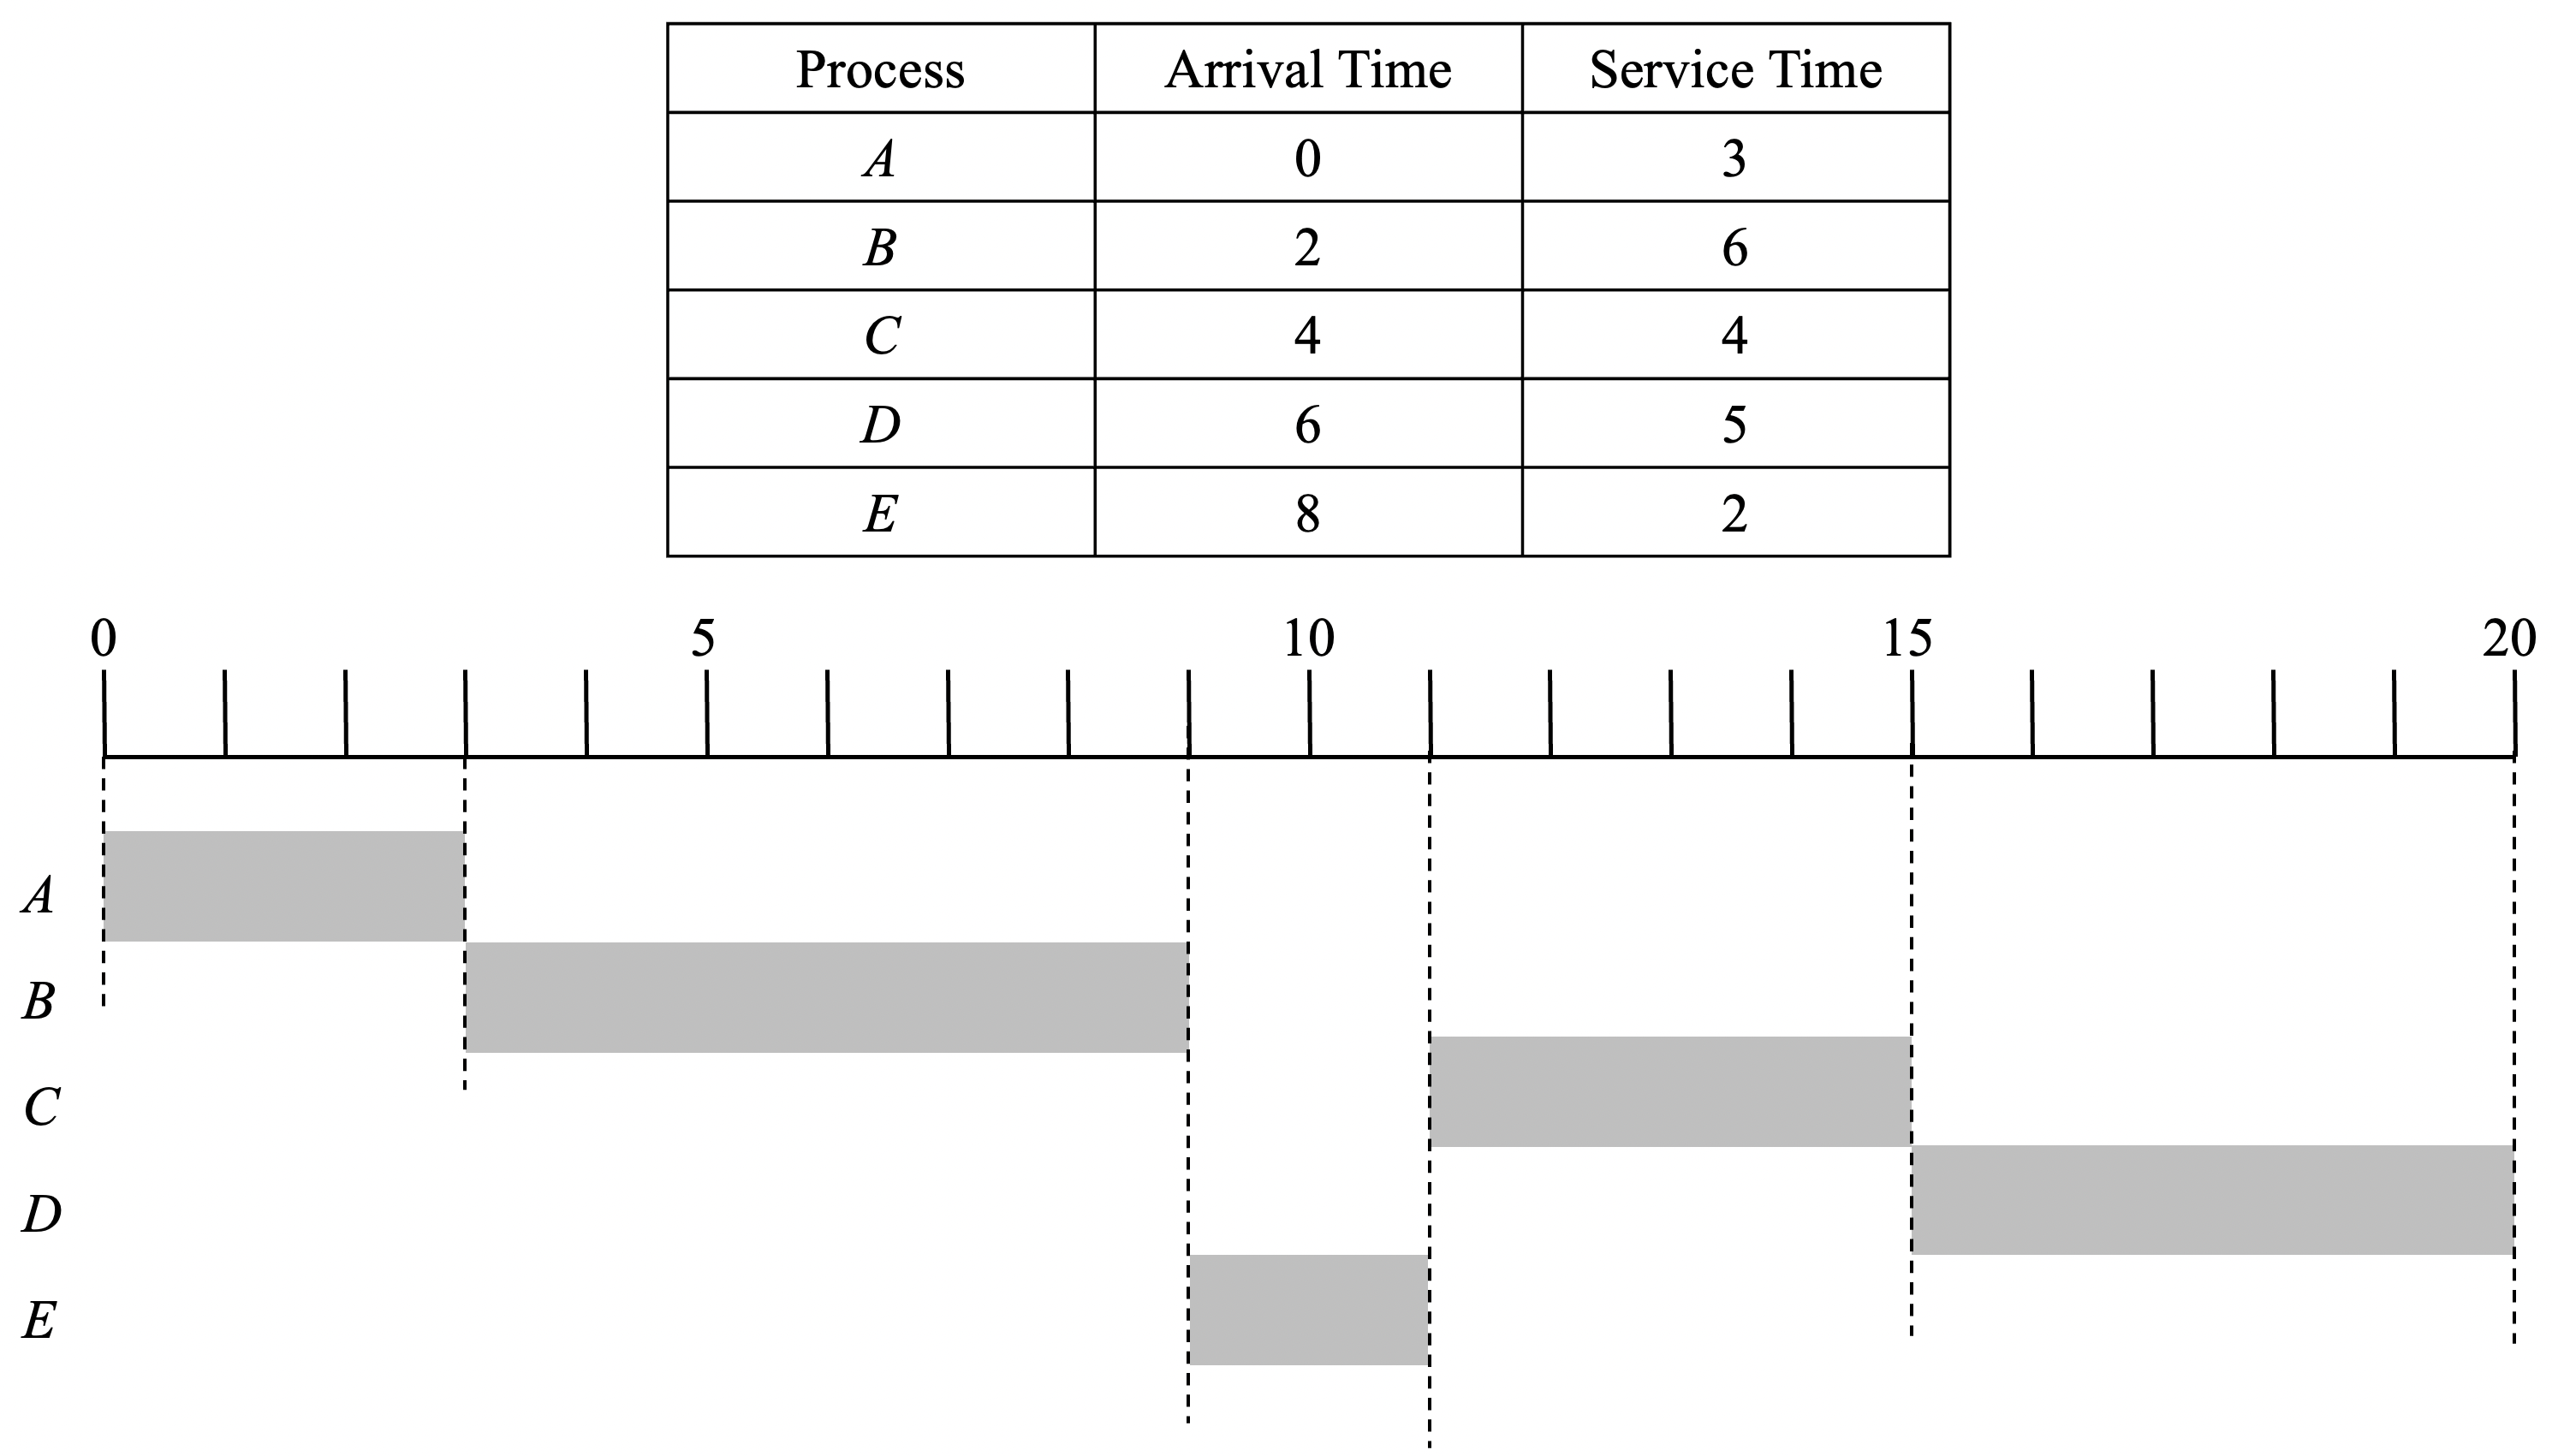
\includegraphics[width=0.7\textwidth]{img/SPF}
	\end{figure}


	\paragraph{最短剩余时间优先SRTF}~{}

	最短剩余时间优先是\textbf{抢占式}调度,类似于 SPF 调度算法,其不公平特征比 SPF 调度算法更加突出
	\begin{figure}[H]
		\centering
		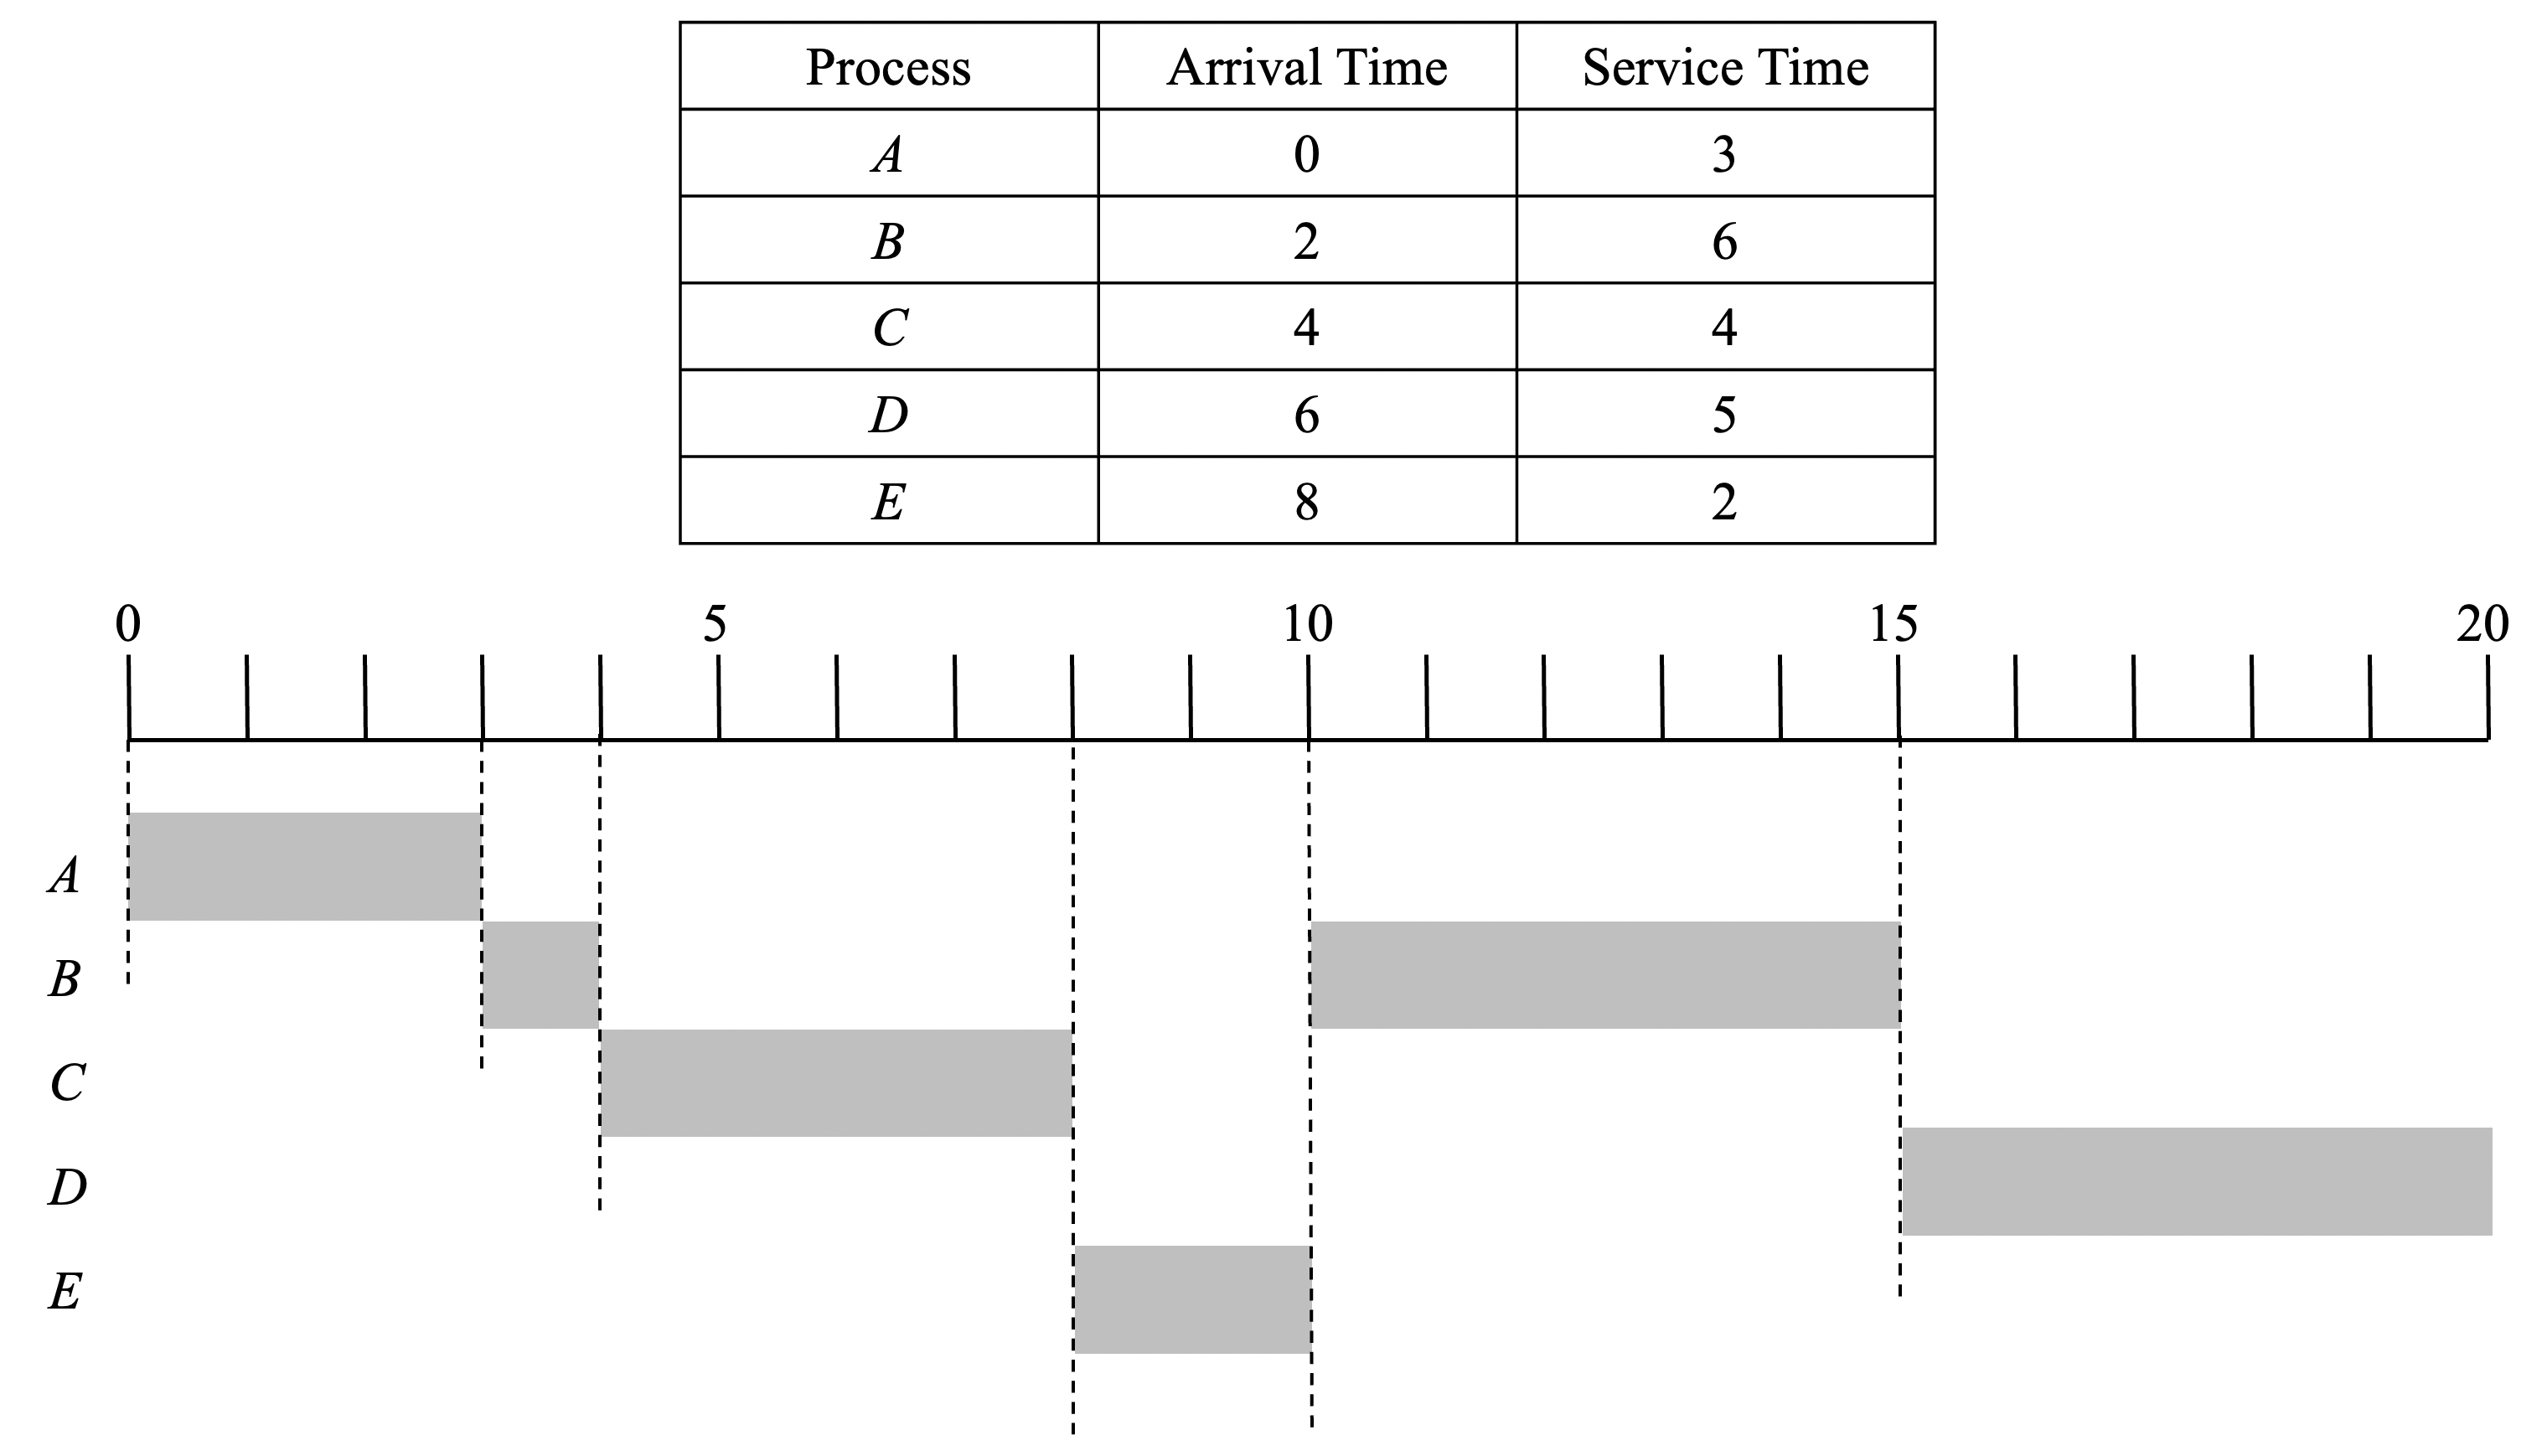
\includegraphics[width=0.7\textwidth]{img/SRTF}
	\end{figure}

	\paragraph{最高响应比优先HRRF}~{}
	
	最高响应比优先是\textbf{非抢占式}调度,每当需要调度时,计算出所有的响应比,选择响应比最高的执行。响应比是等待时间与计算时间之比,这一算法能够改善 SPF调度算法和 SRTF 调度算法对计算时间长的进程极端不公平的问题
	\begin{figure}[H]
		\centering
		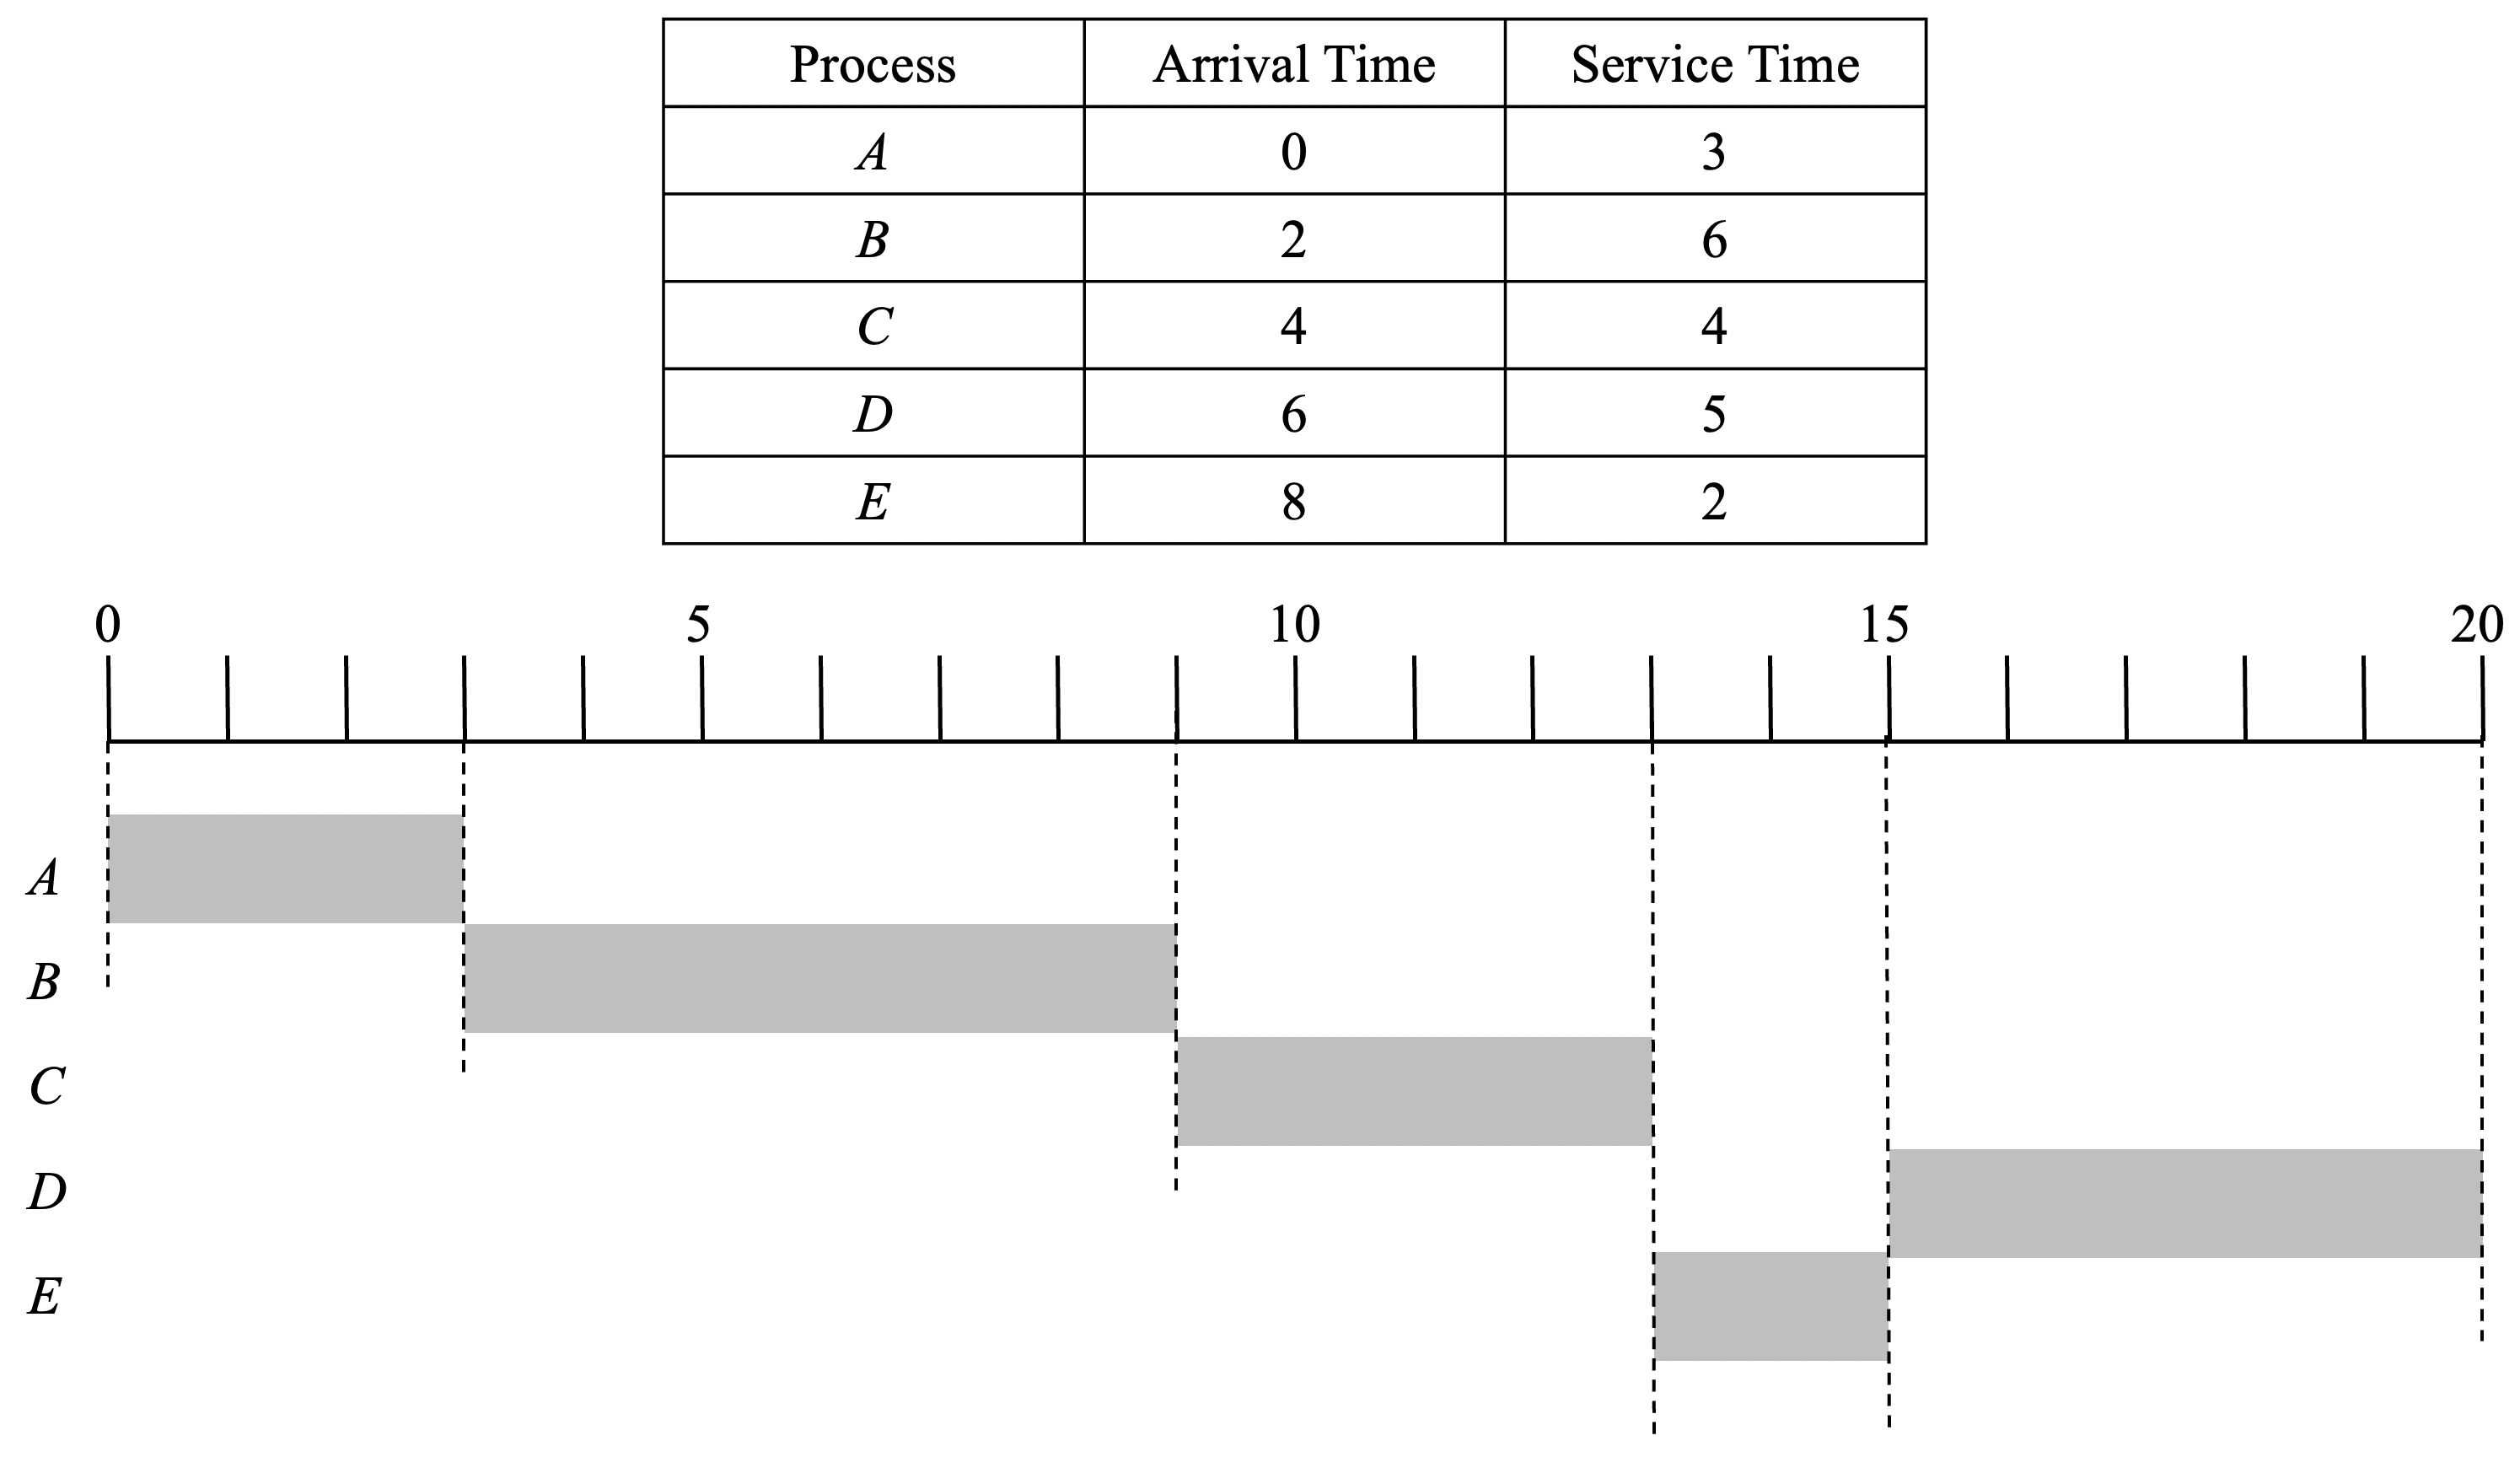
\includegraphics[width=0.7\textwidth]{img/HRRF}
	\end{figure}

	\subsubsection{时间片轮转调度算法}
	时间片轮转(round-rubin scheduling,RR)调度算法是基于先来先服务的,但是每个选程占有 CPU 运行必须受到时间片的限制,一旦进程运行时间超过了该时间片就得让出 CPU

	算法的实现可以设置一个间隔时钟,当进程占有 CPU 时处理器就将间隔时钟设置好,时间到则发出一个间隔时钟中断,操作系统得知该进程的时间片已用完便会让该进程进入就绪队列,从而让出 CPU

	\begin{figure}[H]
		\centering
		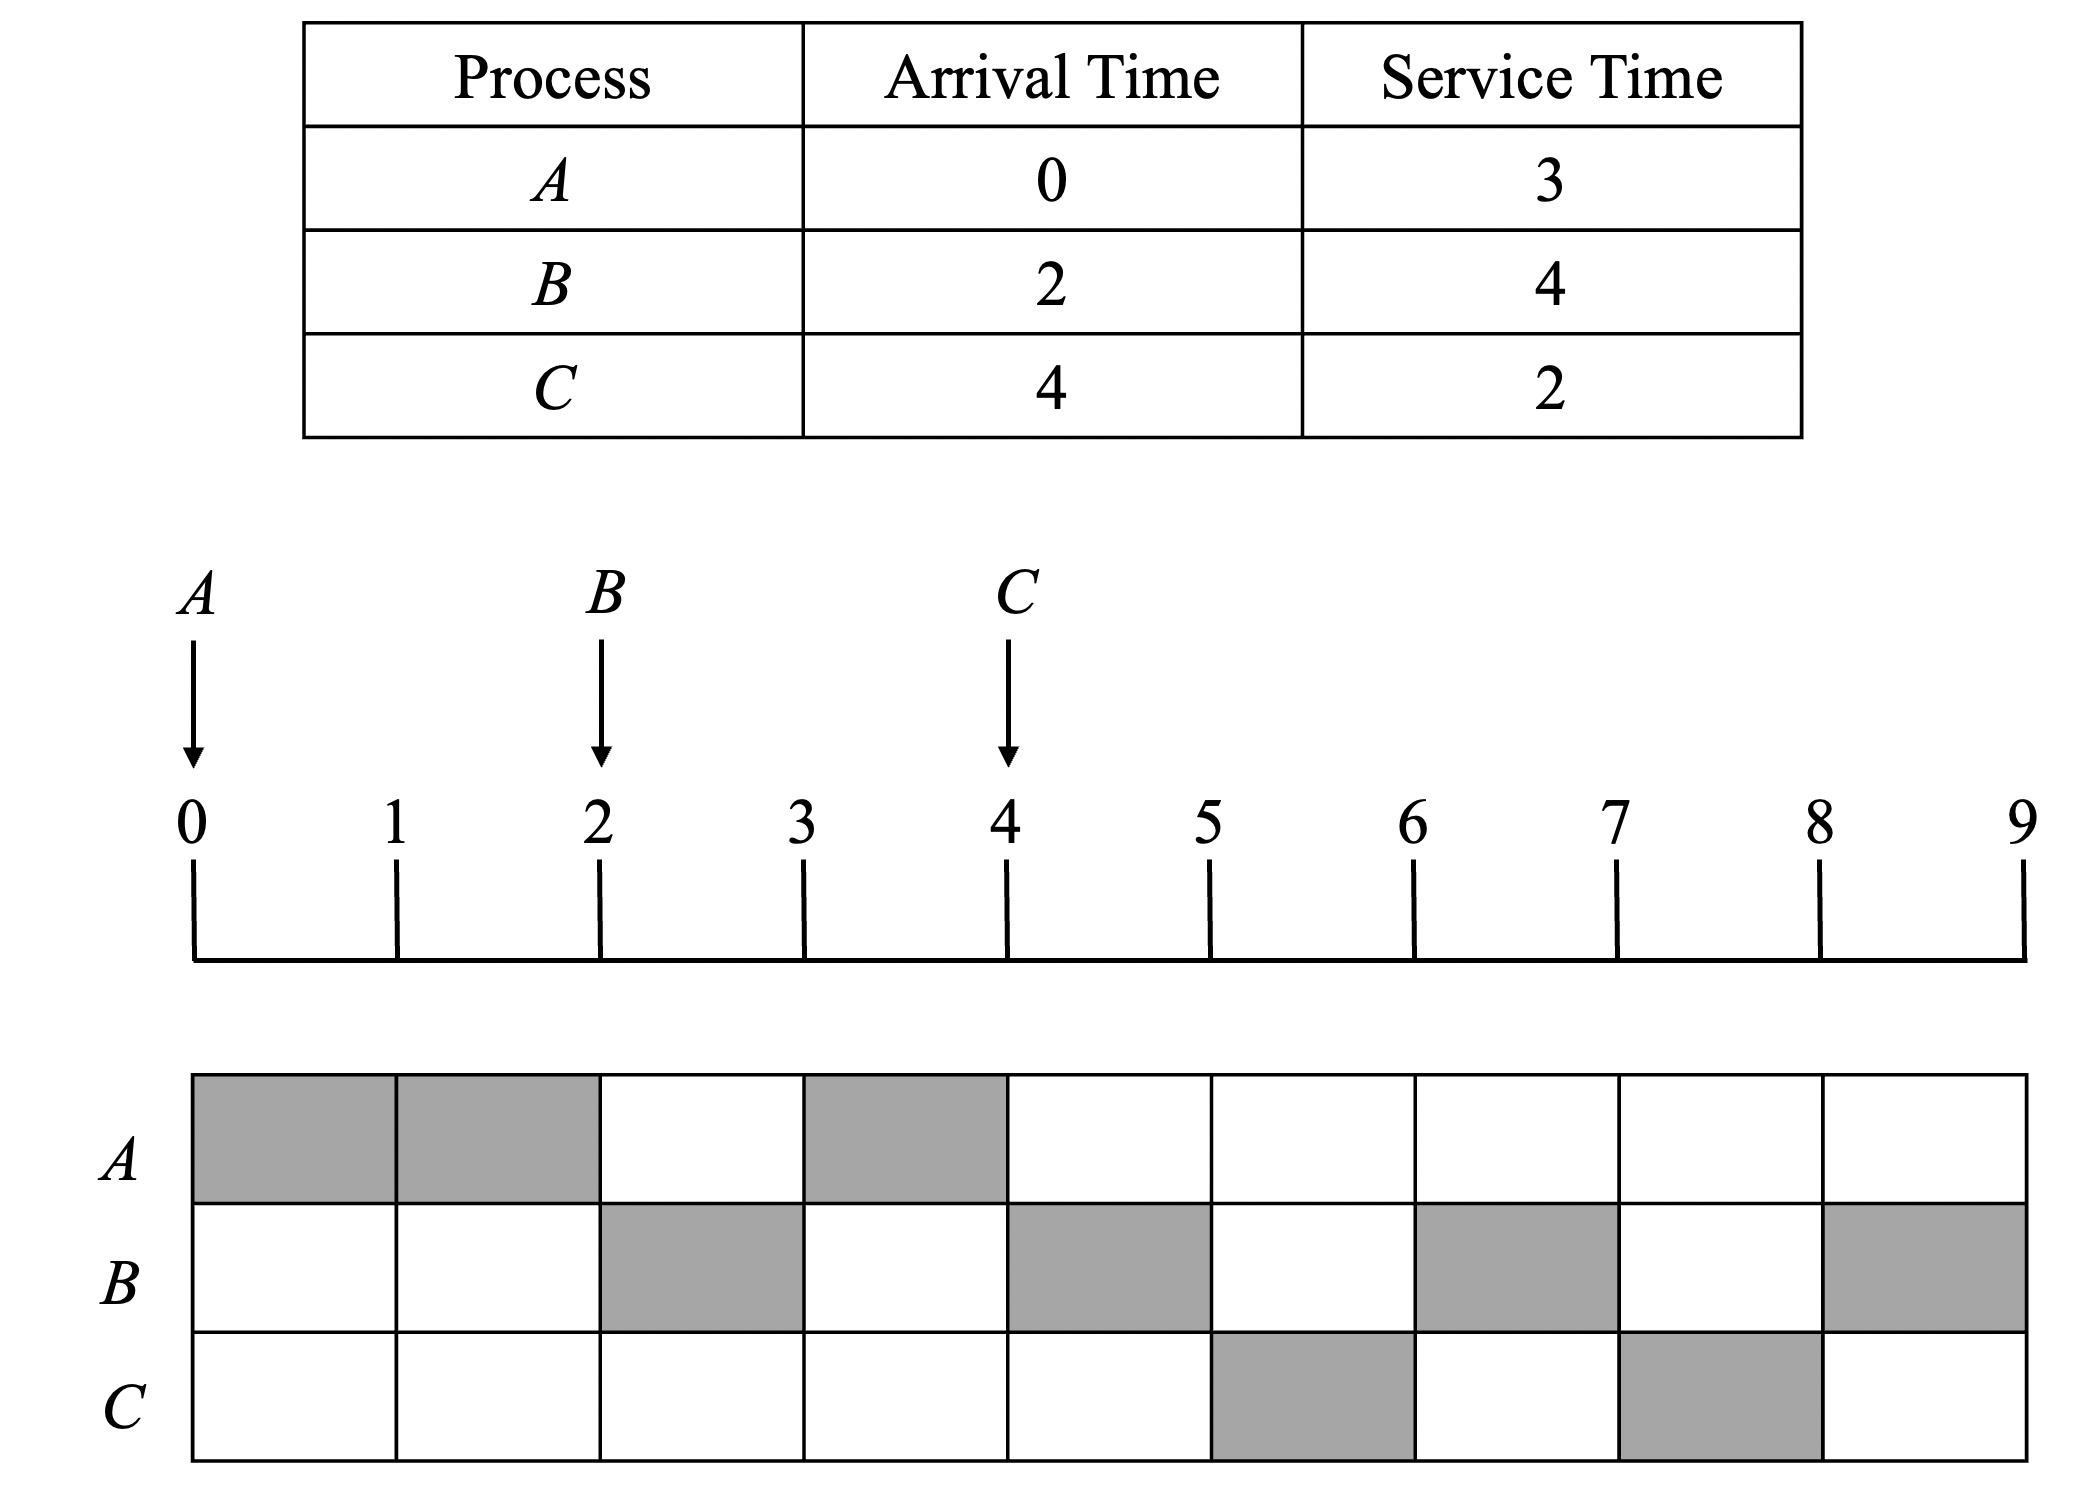
\includegraphics[width=0.7\textwidth]{img/RR}
	\end{figure}

	时间片长度的设置依然是一个难点
	\begin{itemize}
		\item 时间片太长就会退化为先来先服务方式
		\item 时间片太短则会使陷入操作系统的次数人为地增加,系统的代价也比较大
		\item 一般来说,500 ms 或 200ms 是比较合适的时间片长度
	\end{itemize}

	不同的操作系统可以规定一个单一的时间片,也可以为不同的进程规定不同的时间片,甚至根据进程的执行行为动态地调整时间片的长度


	\subsubsection{分级调度算法}
	分级调度算法又称为多级反馈队列(Mulit-level Feedback Queue,MLFQ),基本思想是建立多个按照优先级调度的就绪进程队列
	\begin{itemize}
		\item 多个就绪进程队列之间按照优先数调度
		\item 高优先级的就绪进程分配的时间片短
		\item 单个就绪进程队列中的进程的优先数和时间片相同,按照先来先服务算法调度
	\end{itemize}
	分级原则:外设访问、交互性、时间紧迫程度、系统效率、用户立场

	当一个进程第一次进入系统时,它被放置在 RQ0,当它第一次被抢占后并返回就绪状态时,它被放置在 RQ1。在随后的时间里,每当它被抢占时,它就被降级到下一个低优先级队列中。一个短进程很快会执行完,不会在就绪队列中降很多级

	\begin{figure}[H]
		\centering
		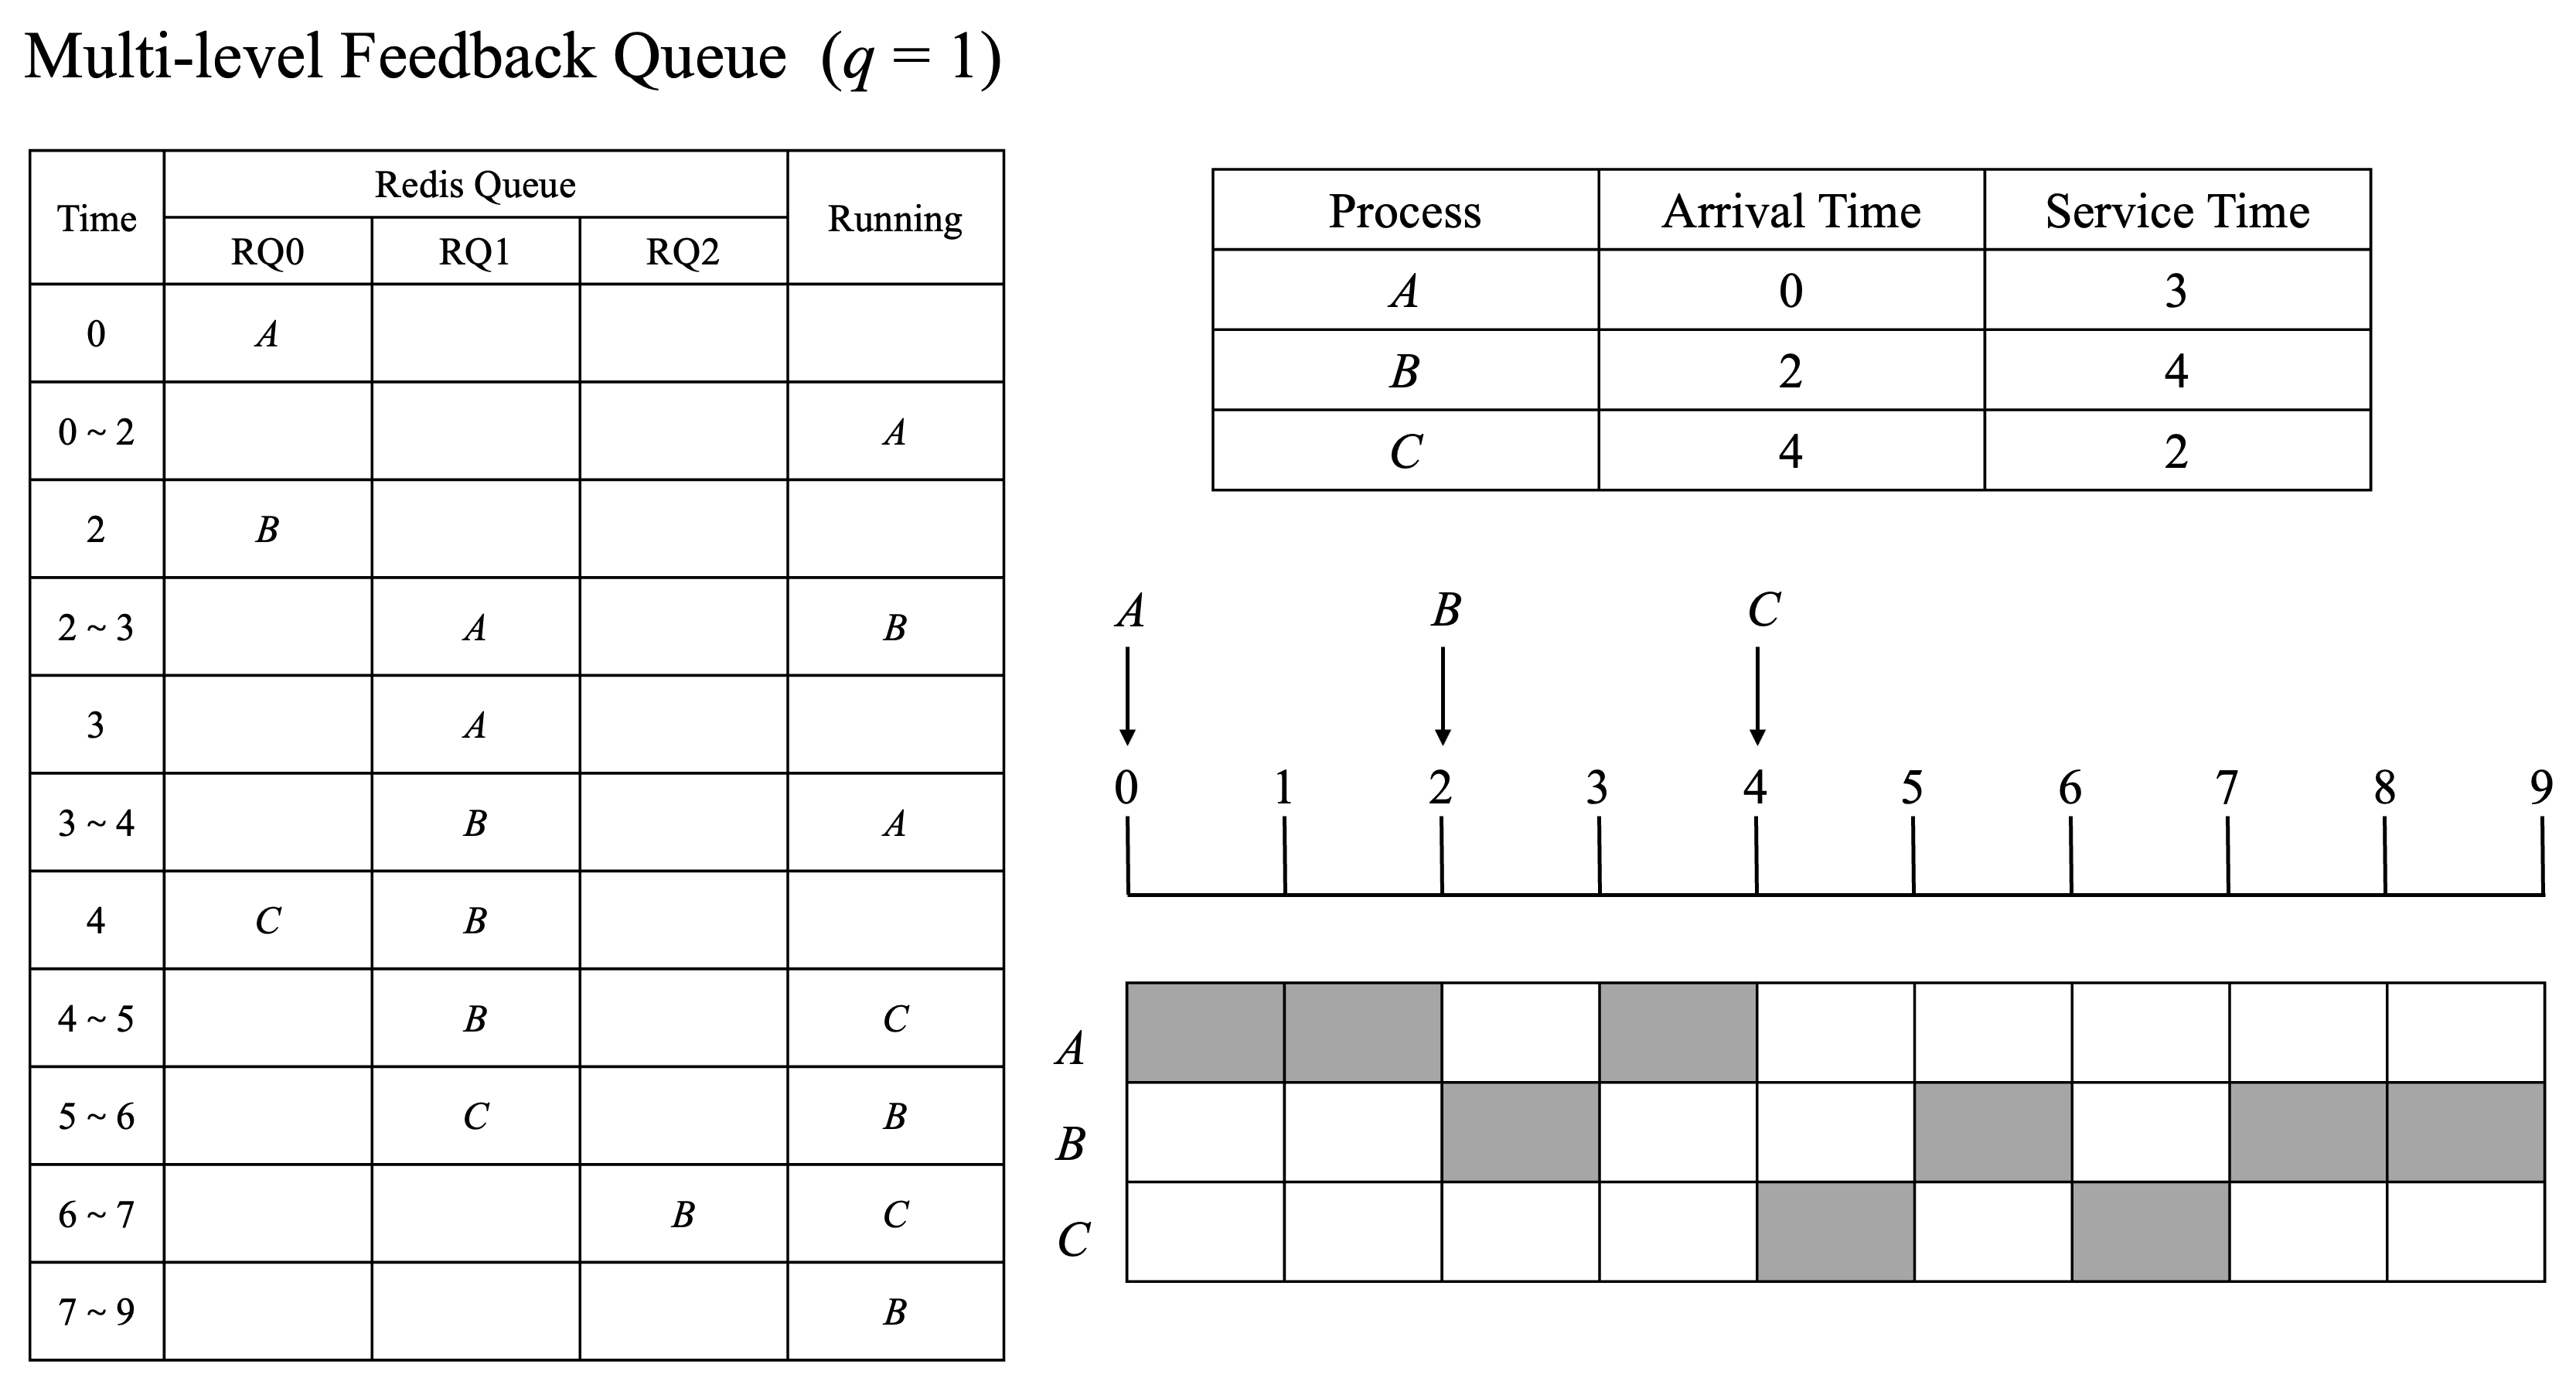
\includegraphics[width=0.95\textwidth]{img/Feedback(q=1)}
	\end{figure}

	不同的进程可以设置不同的时间片长度 $q = 2^i$,其中 $i$ 是层数,即第一层时间片长为 1,第二层长为 2

	\begin{figure}[H]
		\centering
		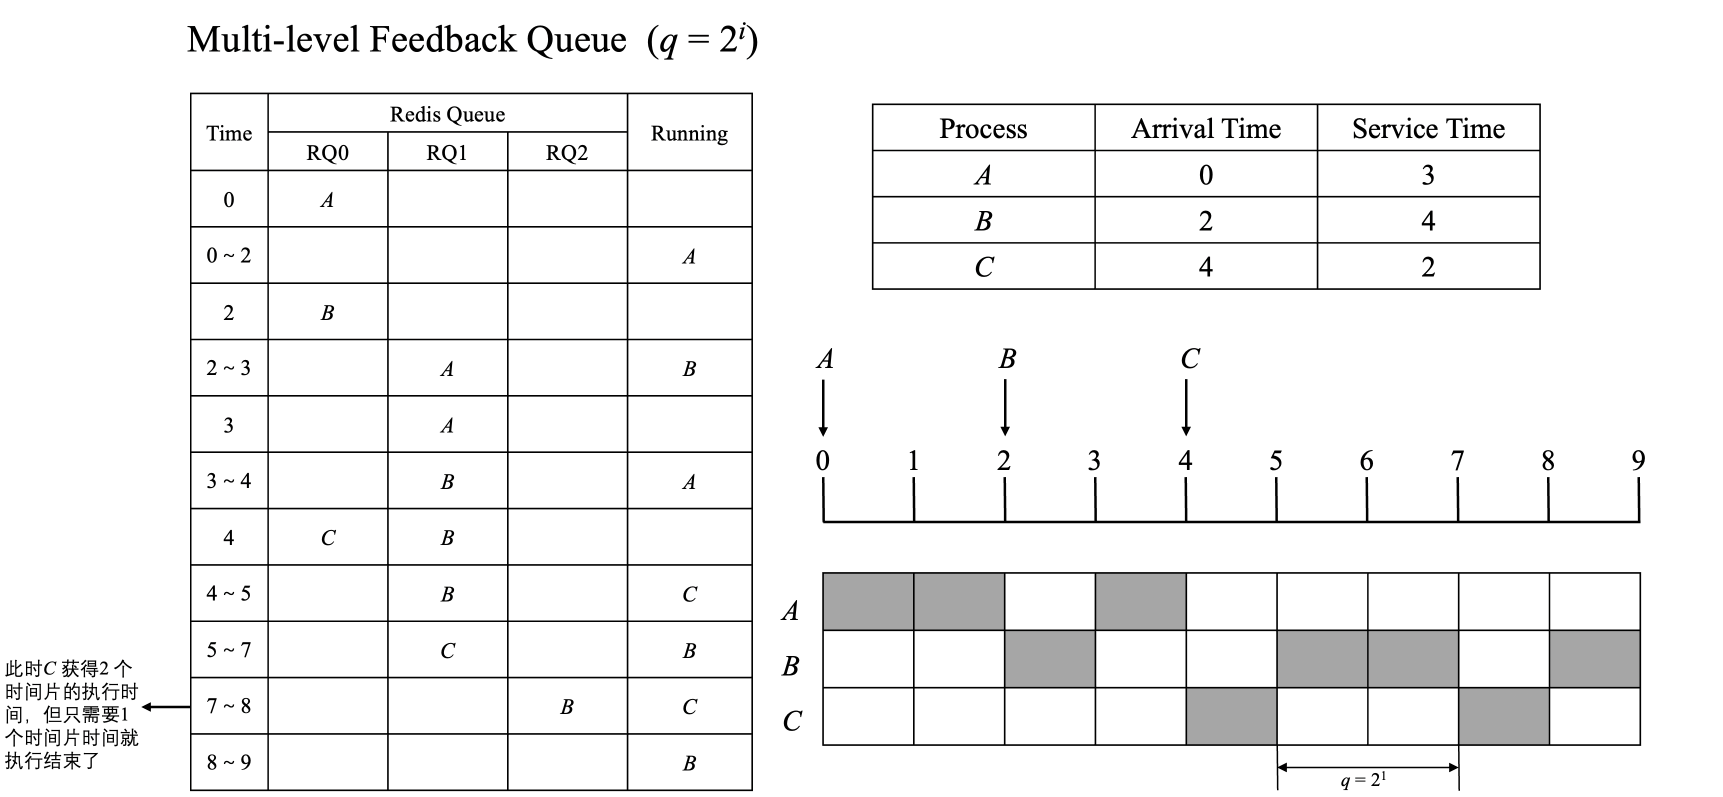
\includegraphics[width=0.95\textwidth]{img/Feedback(q=2^i)}
	\end{figure}

	分级调度算法实例
	\begin{figure}[H]
		\centering
		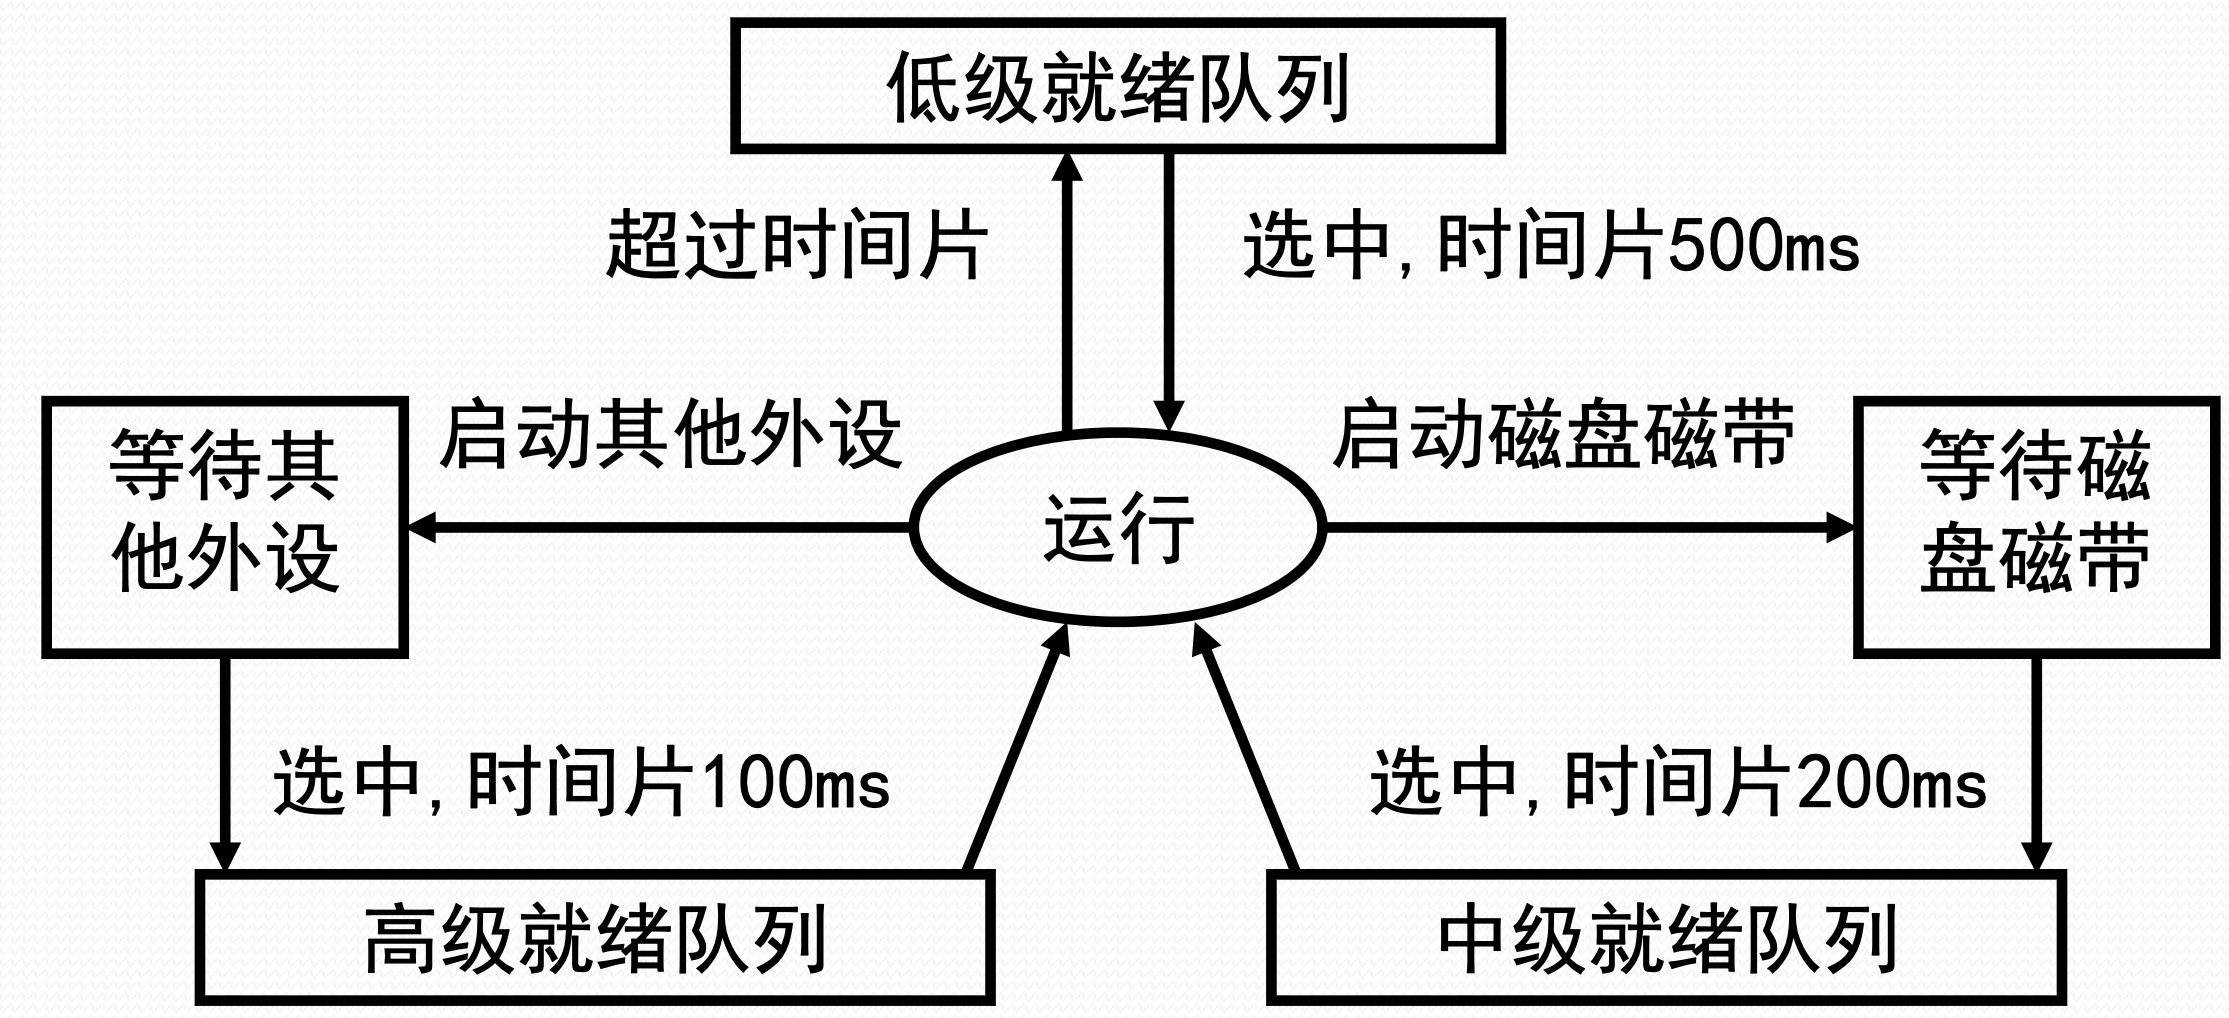
\includegraphics[width=0.6\textwidth]{img/2.5.4}
	\end{figure}

	除了极少数的硬实时操作系统使用抢占式调度算法,绝大多数操作系统有效地组合时间片调度算法和优先数调度算法,采用分级调度算法的策略加以实现
	\begin{itemize}
		\item 处理器首先为实时进程建立若干个高优先数的实时进程队列,如处理网络任务的就绪队列、处理各类软实时任务的就绪队列
		\item 再为交互式分时任务建立一系列进程队列,对于每一个交互式任务,可以设置一个基准优先数,根据执行行为,如访问慢速外设、访问磁盘、超过时间片等,来动态调整它进入的就绪队列
		\item 最后为执行时间紧迫度不高的例行程序设置较低优先数的就绪队列
	\end{itemize}
	现代操作系统的多级反馈队列个数非常多,可以多达 32 个,甚至 128 个

	\subsubsection{彩票调度算法}
	\begin{itemize}
		\item 基本思想:为进程发放针对系统各种资源(如 CPU 时间)的彩票,当调度程序需要做出决策时,随机选择一张彩票,持有该彩票的进程将获得系统资源
		\item 合作进程之间的彩票交换
		\item 一般不会在实时操作系统中使用,但是可以在服务器端进行使用,特别是视频点播服务器
	\end{itemize}

	\subsubsection{Unix SVR4调度算法}
	\begin{figure}[H]
		\centering
		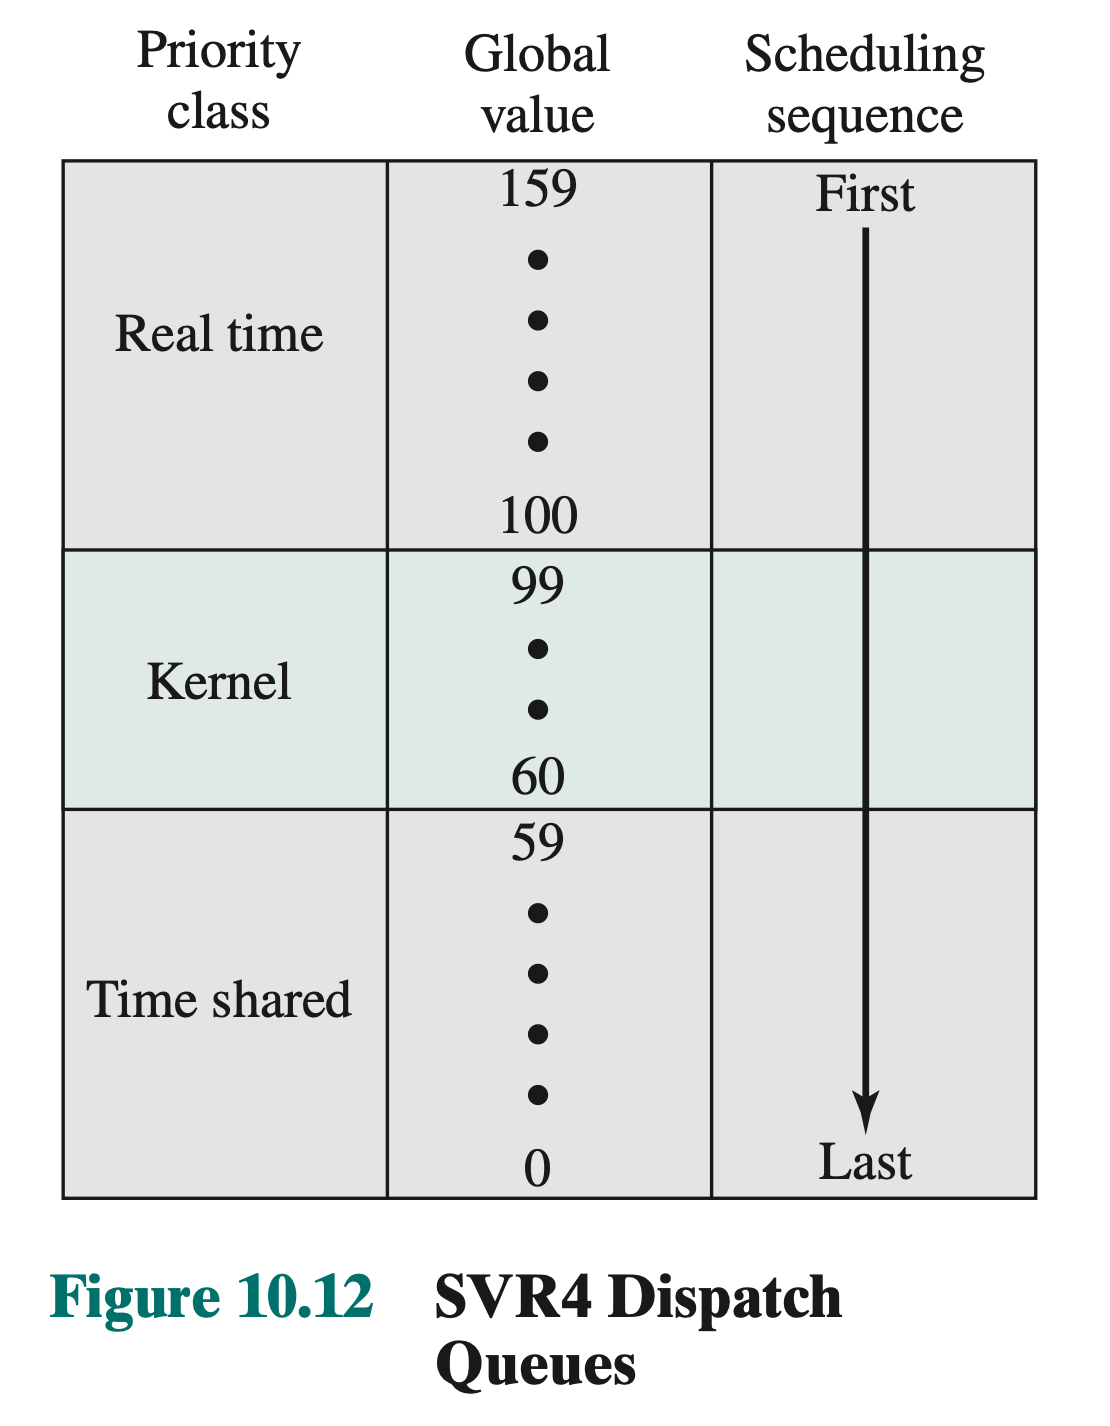
\includegraphics[width=0.3\textwidth]{img/2.5.6.1}
	\end{figure}

	\begin{itemize}
		\item 100$\sim$159 是实时部分任务
		\item 60$\sim$99 是内核部分任务
		\item 0$\sim$59 是分时部分任务
		\item 多级反馈队列,每一个优先数都对应于一个就绪进程队列
		\begin{itemize}
			\item 实时优先级层次:优先数和时间片都是固定的,在抢占点执行抢占
			\item 分时优先级层次:优先数和时间片是可变的,从 0 优先数的 100ms 到 59 优先数的 10ms
		\end{itemize}
	\end{itemize}

	\begin{figure}[H]
		\centering
		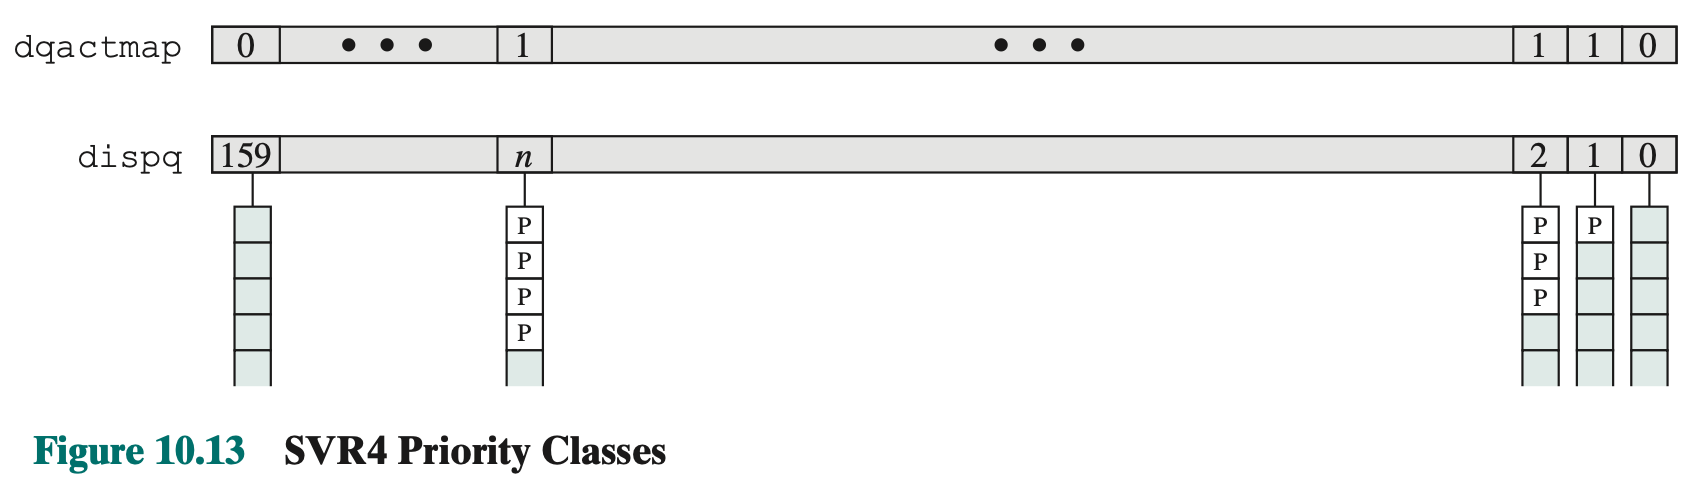
\includegraphics[width=0.8\textwidth]{img/2.5.6.2}
	\end{figure}

\end{document}



